% KU defaults
\documentclass[11pt, a4paper]{article}
\usepackage[english, science, titlepage, dropcaps]{ku-frontpage}
\usepackage[utf8]{inputenc}

% Additional packages
\usepackage{lipsum}
\usepackage{cite}
\usepackage[toc,page]{appendix}
\usepackage{listings}
\usepackage{xcolor}
\usepackage{footnote}
\usepackage{subcaption}
\makesavenoteenv{tabular}
\makesavenoteenv{table}

% KU settings
\setlength\arraycolsep{2 pt}
\setcounter{tocdepth}{2}
% \setcounter{secnumdepth}{0}

% User settings
\lstloadlanguages{C,C++,csh,Java}
\makeatletter
\newcommand\footnoteref[1]{\protected@xdef\@thefnmark{\ref{#1}}\@footnotemark}
\makeatother

\usepackage{color}
\definecolor{bluekeywords}{rgb}{0.13,0.13,1}
\definecolor{greencomments}{rgb}{0,0.5,0}
\definecolor{redstrings}{rgb}{0.9,0,0}

\usepackage{listings}
\lstset{language=[Sharp]C,
  showspaces=false,
  showtabs=false,
  showstringspaces=false,
  breakatwhitespace=true,
  escapeinside={(*@}{@*)},
  commentstyle=\color{greencomments},
  keywordstyle=\color{bluekeywords},
  stringstyle=\color{redstrings},
  basicstyle=\ttfamily,
  breaklines=true,
  postbreak=\mbox{\textcolor{red}{$\hookrightarrow$}\space},
  columns=fullflexible,
  breakatwhitespace=false,
}
\usepackage{caption}
\DeclareCaptionFont{white}{\color{white}}
\DeclareCaptionFormat{listing}{\colorbox{blue}{\parbox{\textwidth}{\hspace{15pt}#1#2#3}}}
\captionsetup[lstlisting]{format=listing,labelfont=white,textfont=white, singlelinecheck=false, margin=0pt, font={bf,footnotesize}}

\assignment{Master thesis}
\author{Martin Thiele}

\title{Banking the unbanked}
\subtitle{Future-proofing the least developed countries as they go from cash to online payment}
% \subtitle{Utilizing current technology to bank the unbanked to support the transition from cash to online payment}
\date{Handed in: \today}
\advisor{Advisors: Fritz Henglein, Søren Terp Hørlück Jessen}
\frontpageimage{figs/phonecashheader.jpg}

\begin{document}

\renewcommand{\bibname}{References}


\maketitle

\begin{abstract}
\noindent Banking is a necessity for everyone, it is a key factor to reduce poverty and is a focal point for many organizations around the world. Unfortunately, 1.7 billion people remain unbanked. We take an example-driven approach to explore the reasons for why this is the case, where this is the case, and how we can bank the people of these countries. We introduce a banking model based on M-Pesa that circumvents some of the complications of the M-Pesa model. In these regions, cash is king. As the digital divide lessens we implement two systems based around this model. One for the current generation, based on the technology already available, and one for future generations, based on technology that will become available. We find that converting from a static agent model to a dynamic one, multiple benefits can appear: The distance to banks is reduced, fees might be reduced, new job opportunities are made, and lack of identification might no longer be a limiting factor.
\end{abstract}

\clearpage

\section*{Acknowledgements}
I would like to thank my co-supervisor, Fritz Henglein, for the invaluable guidance throughout this project. Furthermore, I would like to thank my co-supervisor, Søren Terp Herlück Jessen, for his input on the legal requirements of banking systems. I would also like to thank my brother, Andreas, for helping me ensure the quality of this thesis, and for sparring with me throughout my time at the university. Lastly, I would like to thank my mother, Connie, for always supporting me throughout my education.

\clearpage

\tableofcontents
\clearpage


\section{Introduction}

% Introduce the problem and why banking is necessary
Financial inclusion is the ability to have access to basic banking which includes efficient and secure transactions, trusted ownership, execution of payments, safe storage of money, and withdrawal of cash. This has been defined by The World Bank to be an important building block for both poverty reduction and opportunities for economic growth\cite{gfindex} and is one of the focal points of many international agencies, such as the International Monetary Fund (IMF)\footnote{\url{https://www.imf.org/en/About/Factsheets/IMF-at-a-Glance} - Visited 2021-05-30} and The World Bank\footnote{\url{https://www.worldbank.org/en/what-we-do} - Visited 2021-05-30}, as well as non-profit organizations (NPOs) like the Norwegian Refugee Council (NRC)\footnote{\url{https://www.nrc.no/what-we-do/themes-in-the-field/cash-and-vouchers/} - Visited 2021-05-30}. By having access to these tools societies will see many benefits. In Niger, a five-month relief program swapped from a monthly payment of cash to instead use mobile money services allowing for mobile commerce (m-commerce). This change saved the recipients 20 hours on average in overall travel and wait time to obtain the payments\cite{gfindex}. A similar study was performed in Kenya where the change to mobile money services allowed 185,000 women-headed households to increase their savings by more than 20\%, reducing extreme poverty among these households by 22\%\cite{gfindex}. Additionally, access to digital payments allows for easier storage and a reduction in corruption in countries where trust in the government is low\cite{gfindex}.

\begin{figure}[ht]
\centering
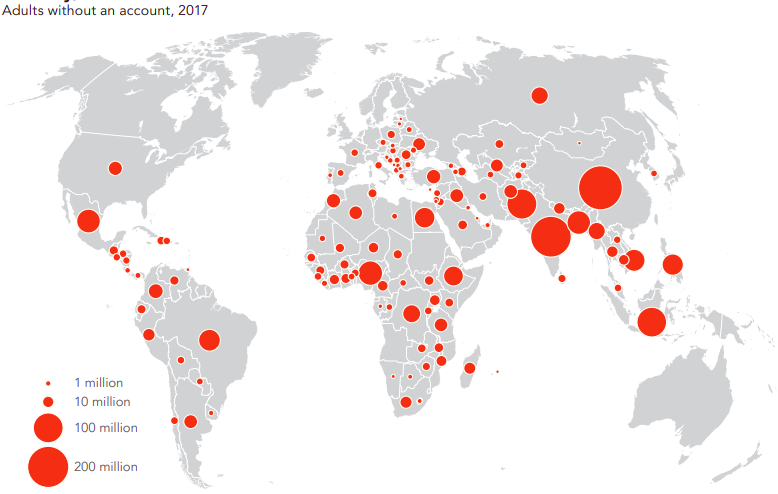
\includegraphics[width=1\linewidth]{figs/unbanked_map}
\caption{\textit{The Global Findex Database}\cite{gfindex}. Map of locations for unbanked adults in 2017.}
\label{fig: unbanked_map}
\end{figure}

The Global Findex Database reports that 69\% of adults in 2017 had a bank account\cite{gfindex}, an increase of 7 percentage points since 2014 and 18 percentage points since 2011\cite{gfindex}. 94\% of adults in developed countries own a bank account, whereas only 63\% of adults own an account in developing countries\cite{gfindex}. Globally, approximately 1.7 billion adults remain unbanked, with half of them living in just seven developing areas: Bangladesh, China, India, Indonesia, Mexico, and Pakistan.

When looking at developing countries and financial technology (fintech) it is important to consider what technologies are available in these areas. 1.1 billion of the financially excluded adults own a mobile phone\cite{gfindex}, however, many developing countries have very little internet access. Our World in Data reports that for the majority of the countries in Sub-Saharan Africa (SSA), one of the least developed regions, the population with access to the internet is only between 5 and 20\%\cite{owidinternet}, however for most of these countries, the mobile phone penetration rate\footnote{The mobile phone penetration rate refers to the amount of SIM cards in a certain country} is greater than 40\%\cite{owidinternet}.

Banking the unbanked is a \$380 billion revenue opportunity\footnote{\url{https://www.accenture.com/us-en/\_acnmedia/Accenture/Conversion-Assets/DotCom/Documents/Global/PDF/Dualpub\_22/Accenture-billion-reasons-bank-inclusively.pdf} - Visited 2021-05-30} which has seen an increase in interest throughout the last decade, mainly due to the success M-Pesa has had in Kenya. The potential revenue lies in converting the usage of cash, to the usage of online payments, thereby taking a fee of the transactions, as well as allowing for m-commerce (mobile) and e-commerce (electronic) as the digital divide lessens in the developing countries. McKinsey\cite{mckinsey}, as well as the UN\footnote{\url{https://www.un.org/africarenewal/magazine/may-july-2017/africa\%E2\%80\%99s-quest-cashless-economy-gains-momentum} - Visited 2021-05-30} notes that developing countries such as Argentina, India, Indonesia, Mexico, as well as the countries in SSA, have between 72\% and 96\% of all transactions completed through the usage of cash, whereas mature markets such as the USA, the Netherlands, and Scandinavia, only transact through cash between 9\% and 28\% of the time.

This thesis will contribute to existing research by proposing a modification of existing technologies within the field of banking the unbanked. We hope to solve some of the complications surrounding the existing models such that developing countries can transition effectively into the digital world, thereby allowing for a better economy.

In this thesis we will take an example-driven approach of defining the needs and requirements of a mobile banking application, as well as determine the country with the largest need to onramp such a project, ensuring that the targeted country's needs, likewise, are met. When the requirements are defined we will implement a basic bank meeting these requirements, utilizing the technology that is available to them, with features that allow for any user to see the benefits of entering the mobile bank network. We will then evaluate the use cases of this product and the important variables of the product, before performing a security analysis looking at the potential attack vectors of the mobile bank. We will then discuss the implementation and reason for our choices before taking a look at the existing work done within this field which we have drawn inspiration from. Finally, we will conclude with our findings.


\section{Analyzing the needs of a banking service}
\subsection{The regions in need of becoming banked}
To start deternining which region is worth exploring further, we take a look at the statistics revolving around financial inclusion in the different parts of the world.
\begin{table}[!ht]
\begin{tabular}{|l|l|l|l|}
\hline
\textbf{Region}       & \textbf{Account (\%)} & \textbf{FI\footnote{Financial institution account}(\%)} & \textbf{M\footnote{Mobile money account} (\%)} \\ \hline
East Asia \& Pacific    & 70.6          & 70.3           & 1.3                \\ \hline
Europe \& Central Asia    & 65.3          & 65.1           & 3.2                \\ \hline
Latin American \& Caribbean & 54.4          & 53.5           & 5.3                \\ \hline
The Middle East \& North Africa & 43.5          & 43.0           & 5.8                \\ \hline
South Asia          & 69.6          & 68.4           & 4.2                \\ \hline
Sub-Saharan Africa      & 42.6          & 32.8           & 20.9                 \\ \hline
\end{tabular}
\caption{Financial inclusion statistics from six regions of the world, aged 15 and up\cite{littledata}}.
\label{tab:financial_statistics}
\end{table}

We can from \autoref{tab:financial_statistics} and \autoref{fig: unbanked_map} deduce that the majority of the financially excluded people are located in the Middle East \& North Africa (MENA) (43.5\%), and Sub-Saharan Africa (42.6\%), whereas only 32.8\% of the people in SSA are banked through traditional means. 20.9\% are banked through mobile money accounts, showing a clear need for a fintech solution in these regions.

There are many possible approaches to consider when contemplating the implementation of a banking system, e.g. Bluetooth-based, blockchain-based, EMV cards (Debit and credit cards). To determine which approach, and which of the two regions have the best infrastructure to support the different approaches we will analyze them based on the following parameters:
\begin{itemize}
   \item \textbf{Mobile phone penetration rate}

   The relative amount of active cellular subscriptions in the region
   \item \textbf{Smartphone penetration rate}

   The relative number of active smartphones in the region
   \item \textbf{Cost of entry-level internet-enabled device}

   The cost of a simple smartphone (in GDP per capita)

   \item \textbf{Data affordability}

   The price for 100 MB of data (in monthly GDP per capita)

   \item \textbf{Mobile infrastructure (Rural)}

   How well the rural parts of the regions are covered by 2G, 3G, and 4G mobile internet.

   \item \textbf{Mobile infrastructure (Urban)}

   How well the urban parts of the regions are covered by 2G, 3G, and 4G mobile internet.

   \item \textbf{Internet download speed}

   \item \textbf{Barriers from being banked}

   \item \textbf{Currently utilized banking services}
 \end{itemize}

\noindent The mobile phone penetration rate was generally between 40-75\% in SSA in 2017, with some countries above 80\% and a few above 120\%\cite{owidinternet}, suggesting that people have more than one cellular subscription. In Africa, this isn't uncommon due to several factors:
\begin{itemize}
  \item Carriers attempt to attract subscribers with special deals, e.g. unlimited SMS (Short Message Service), cheaper network calls, bonus monthly data plans\footnote{\url{https://www.theafricareport.com/14567/} \label{fn1} }.
  \item Costs of services matter a lot, particularly in poor countries, as such swapping between providers can be a lucrative investment.\textsuperscript{\ref{fn1}}
  \item Network reception might be poor in remote areas of Africa, as such, another network might have better coverage in the given area.\textsuperscript{\ref{fn1}}
\end{itemize}
In MENA however, the majority of countries have a rate above 100, with only a few countries, such as Iraq, around the 80s.

 The smartphone penetration rate was 45\% in SSA in 2018, with a projected increase to 67\% in 2025. The same rate was 57\% in MENA, with a projected increase to 74\%\cite{gsmame}, suggesting that a smartphone implementation might not meet the requirements that SSA and MENA currently have, since implementing such a system would cut off the majority of its potential users in SSA. An entry-level smartphone in SSA costs 4.6\% GDP per capita and 2.5\% GDP per capita in MENA, making these devices fairly expensive. For comparison, a similar device costs 0.8\% GDP per capita in South America\cite{gsma}.

Internet and the cost of internet data are important factors for any implementation requiring internet, as such data affordability will have to be taken into account. In SSA, 100MB of data costs 4.3\% of the monthly GDP per capita in 2017, a decrease from 2014's 8.6\%. In MENA the same data is 0.7\% of the monthly GDP per capita, which in 2014 was 1.2\%\cite{gsma}. The infrastructure to support the internet in these regions exist, but could be better. In rural Africa, the continent is covered by 22\% 4G internet, 40\% 3G internet, and 18\% 2G internet, making 20\% of rural Africa inaccessible, whereas 77\% of urban Africa is covered by 4G and the last 23\% by 4G. The rural parts of the Arab States, are covered by 44\% 4G internet, 34\% 3G internet and 10\% 2G internet, leaving 12\% of the region inaccessible. Quite similar to Africa, 78\% of the urban Arab States are covered by 4G internet, with the remaining 22\% covered by 3G\cite{ituinternet}. Internet speeds have become better from 2014 through 2017, further closing the gap being the developing countries and the developed ones. In SSA the average download speed was 0.5 Mbps in 2014, which has increased to 2.4 Mbps in 2017. Similarly, MENA has increased from 2.0 Mbps to 7.6 Mbps\cite{gsma}.

To summarize on the infrastructure, both regions have mobile phones available to them and a future of smartphones. SSA and MENA have both progressed well from 2014 to 2017, by providing cheaper data and faster internet. The internet accessibility is good, with 3G or 4G covered in urban SSA and urban MENA, but with some rural areas not yet covered. With the infrastructure to support at least mobile phones, but not yet ready for smartphones, let's determine why the people aren't banked already.

\begin{table}[!ht]
\centering
\begin{tabular}{|l|l|l|}
\hline
\textbf{Reason} & \textbf{SSA (\%)} & \textbf{MENA (\%)} \\ \hline
Distance to bank & 19 & 5 \\ \hline
Services are too expensive & 19 & 12 \\ \hline
Lack of necessary documentation & 18 & 7 \\ \hline
Lack of trust in financial institutions & 10 & 7 \\ \hline
Religious reasons & 4 & 4 \\ \hline
Insufficient funds & 51 & 44 \\ \hline
A family member has an account & 8 & 7\\ \hline
\end{tabular}
\caption{Reasons for lack of financial accounts in SSA and MENA\cite{gfindex}}
\label{tab:ssa_mena_reasons}
\end{table}

from \autoref{tab:ssa_mena_reasons} we can see that distance is a problem for almost one-fifth of all the unbanked people in SSA, whereas this isn't a major concern for the citizens in MENA.

Service costs are a problem for both regions, but seeing how SSA consists of a lot of developing countries with a poor GDP, it's SSA that leads this statistic.

18\% of SSA lack the identification necessary to become banked, and banks are known to not take such risks. World Bank Group\cite{worldbankid} reasons that people don't have an id due to the fee costs revolving around obtaining one. Often fees can cost upwards of 8-10 US Dollars\cite{worldbankid}, with an additional cost for travel costs and supporting documentation\cite{worldbankid}. Additionally, lack of an id is often not a barrier in the peoples day to day life\cite{worldbankid}.

Both regions lack trust in financial institutions to a lesser degree than the previous reasons, this is understandable for both regions, particularly SSA who have had a history of corrupt governments, to this day, corruption is still at large in some SSA countries. With the COVID-19 pandemic, the distrust in governments further increased due to mishandling of funds, overpricing, as well as hoarding of COVID-19 medication\cite{cpi2020}.

4\% in SSA and MENA reason that religious reasons are a cause for them not to be banked. Many countries in SSA and MENA are highly religious but only a few of them list religion as a concern. Niger is a Muslim-dominant country with 98.4\% of the population being Muslim\cite{muslim} and 21\% reasoning that religion prohibits them from being banked\cite{gfindex}. Islamic finance comes with a set of rules which should be in accordance with Islamic law, particularly lending with interest is prohibited since it is deemed exploitative to earn money from interest\footnote{\url{https://www.investopedia.com/articles/07/islamic\_investing.asp} - Visited 2021-05-30}.

The majority reason for both regions is the lack of funds to enter a bank, as such, to provide banking services for the poorest people in the world, the service has to be cheap, and there need to be additional reasons for them to become banked.

Lastly, 8\% and 7\% respectively cite that they don't have an account because a family member has one, this can be explained by the service cost of being banked, or because of financial literacy issues. In general, the amount of education in SSA is very low with some countries having less than two years of schooling on average\cite{hdr}. The education level is overall better in MENA\cite{hdr}.

Overall MENA has very few reasons to not be banked other than the lack of funds, what hinders the region from mobile banks however is regulations. Most countries across MENA haven't allowed non-banks to launch mobile money services.\cite{gsmareg}

SSA is already thriving with mobile bank services. Many mobile network operators attempt to replicate the success of M-Pesa, utilizing their already existing mobile network to support Unstructured Supplementary Service Data (USSD), as well as local mom-and-pop shops to act as agents providing the service of depositing and withdrawing. We reason that there are other potential means of providing a banking service with the existing technology available, however, before settling on implementation we will focus our scope on finding a specific country in SSA since the regulations in MENA prohibit non-banks from providing banking services.



\subsection{Determining the best-suited country} % (fold)
\label{sub:determining_the_best_suited_country}
Similar to how we determined the most-suited region, we will take an analytic approach to who has the biggest need, as well as best infrastructure by looking at the following attributes:

\begin{itemize}
  \item Country specifics
  \begin{itemize}
  \item Population size
  \item Surface Area
  \item Population density
  \end{itemize}
  \item Financial specifics
  \begin{itemize}
  \item GDP per capita
  \item Percentage owning a financial institution account
  \item Percentage owning a mobile money account
  \item Percentage financially included
  \end{itemize}
  \item Population specifics
  \begin{itemize}
  \item Average years of schooling
  \item Literacy level
  \item Financial literacy level
  \item Mobile phone penetration rate
  \item Internet penetration rate
  \item Reasons for being unbanked
  \end{itemize}
\end{itemize}
Lastly, as we draw closer to a feasible target, we will investigate the country's history and specific points of interest that might be relevant, such as regulations.

\begin{table}[!ht]
\centering
\begin{tabular}{|l|l|l|l|}
\hline
\textbf{Country}        & \textbf{M (\%)} & \textbf{FI (\%)} & \textbf{Financial inclusion (\%)} \\ \hline
Burundi             & 0.7            & 7.0                      & 7.0                  \\ \hline
Central African Republic    & 0.0            & 13.7                       & 13.7                  \\ \hline
Chad              & 15.2             & 8.8                      & 21.8                 \\ \hline
Congo, Democratic Republic of & 16.1             & 15.0                       & 25.8                  \\ \hline
Ethiopia            & 0.3            & 34.8                       & 34.8                  \\ \hline
Guinea            & 13.8             & 14.6                       & 23.5                  \\ \hline
Madagascar          & 12.1             & 9.6                      & 17.9                  \\ \hline
Mauritania          & 4.0            & 19.0                       & 20.9                  \\ \hline
Niger             & 8.7            & 9.5                      & 15.5                  \\ \hline
Sierra Leone          & 11.0             & 12.4                       & 19.8                  \\ \hline
South Sudan           & 0.0            & 8.6                      & 8.6                  \\ \hline
\end{tabular}
\caption{Financial inclusion statistics for some of the 11 most financially excluded countries in SSA\cite{gfindex}.}
\label{tab:financial_statistics_ssa}
\end{table}
By comparing the amount of financially included with the average of the region, as well as comparing the number of mobile money accounts with the amount of financially included, we discover just 11 countries. The financial specifics of these countries can be found in \autoref{tab:financial_statistics_ssa}.


The technology infrastructure is an important factor. We reason that a device capable of transferring information is a necessity. As such we will exclude any country with a low mobile phone penetration rate. By removing any country below the average of 55.51 from \autoref{tab:mob_internet_ssa}, we filter down to just four countries: Burundi, Guinea, Mauritania, and Sierra Leone. The internet rate is at 21.83\% at its best in Guinea, as such, a banking model requiring the internet is not favorable.

\begin{table}[ht]
\centering
\begin{tabular}{|l|l|l|l|}
\hline
\textbf{Country}        & \textbf{Mobile (\%)} & \textbf{Internet (\%)} \\ \hline
Burundi             & 56.65             & 2.66                                        \\ \hline
Central African Republic    & 33.62             & 4.34                                      \\ \hline
Chad              & 48.07             & 6.5                                       \\ \hline
Congo, Democratic Republic of & 42.77             & 8.62                                       \\ \hline
Ethiopia            & 37.22             & 18.62                                       \\ \hline
Guinea            & 100.8             & 21.83                                       \\ \hline
Madagascar          & 40.57             & 4.71                                        \\ \hline
Mauritania          & 104.09            & 20.8                                       \\ \hline
Niger             & 40.64             & 5.25                                        \\ \hline
Sierra Leone          & 86.13             & 13.24                                       \\ \hline
South Sudan           & 20.09             & 7.98                                        \\ \hline
\textbf{Average}        & \textbf{55.51}        & \textbf{10.41}                                        \\ \hline
\end{tabular}
\caption{Mobile\cite{wbdata} and internet\cite{wbdata} penetration in SSA for some of the 11 most financially excluded countries in SSA.}
\label{tab:mob_internet_ssa}
\end{table}


To finally determine a country, we will take a look at them individually, with a special focus on their GDP per capita.

\begin{table}[ht]
\centering
\begin{tabular}{|l|l|l|l|}
\hline
\textbf{Country}        & \textbf{GDP per capita} \\ \hline
Burundi             & 261.2   \\ \hline
Guinea            & 962.8 \\ \hline
Mauritania          & 1,679.4 \\ \hline
Sierra Leone          & 527.5 \\ \hline
\end{tabular}
\caption{GDP per capita\cite{wbdata} among the four remaining, potential countries}
\label{tab:gdp_internet_ssa}
\end{table}

% subsection determining_the_best_suited_country (end)

Burundi is the second poorest country in SSA, only beaten by Somalia\cite{wbdata}. 28.9\%\cite{wbdata} of their GDP comes from Agriculture, with 90\% of the population working in the agriculture section to subsistence\footnote{Country fact sheet on food and agriculture policy trends: Burundi. \url{http://www.fao.org/3/i4909e/i4909e.pdf} - Visited 2021-05-30}. Due to the economy of Burundi, we don't see the country as being ready for mobile money. Furthermore, there is a lack of data explaining why the people are otherwise not banked.

\begin{table}[!ht]
\centering
\begin{tabular}{|l|l|l|l|}
\hline
\textbf{Reason} & \textbf{Guinea (\%)} & \textbf{Mauritania (\%)} & \textbf{SA}\footnote{Sierra Leone} (\%) \\ \hline
Distance to bank & 30 & 16 & 18 \\ \hline
Services are too expensive & 30 & 24 & 28 \\ \hline
Lack of necessary documentation & 38 & 19 & 29 \\ \hline
Lack of trust in financial institutions & 15 & 9 & 10 \\ \hline
Religious reasons & 11 & 6 & 4 \\ \hline
Insufficient funds & 74 & 51 & 78 \\ \hline
A family member has an account & 8 & 13 & 4\\ \hline
\end{tabular}
\caption{Reasons for lack of financial accounts for Guinea, Mauritania, and Sierra Leone\cite{gfindex}}
\label{tab:ssa3_reasons}
\end{table}


Guinea has a decent GDP per capita, it has the second-highest mobile phone penetration rate, with more than 100 active SIM subscriptions per 100 residents. They have the greatest amount of active users of the internet among the 11 countries. 13.8\% of citizens are already banked through mobile banking. A bank service in Guinea should, based around the reasons listed in \autoref{tab:ssa3_reasons}, be nearby, cheap, and if possible, allow for the unidentifiable to become banked.

Mauritania is the richest of the selected countries, the people surveyed by the Global Findex Database\cite{gfindex}, list few reasons as to why they are unbanked. They don't seem to have as large a need for a bank as the Guineans.

Lastly, Sierra Leone. Sierra Leone is a poor country, still recovering from a civil war in 2002. They have the infrastructure for a mobile-targeted banking service, as well as a growing amount of internet users. The majority of the people financially included are already included through mobile banks.

While both Mauritania and Sierra Leone have the structure required for a mobile-based banking system, we determine that Guinea has the largest need, as well as a well enough economy for a current, and future, need. We'll utilize the remaining attributes as knowledge for the next chapter, where we will determine the product requirements.

Guinea is a population-dense country, with a population per km$^2$ of 51.94\cite{wbdata} spread over the 245,860km$^2$ surface area. The people are mainly located around the capital of Conakry and the west coast. The average years of schooling is in the extreme lows of 2.6\cite{owidliteracy}, which explains why their literacy level is only 30\%, meaning that only 30\% of those older than 14 years of age are capable of reading and writing\cite{owidliteracy}. Lastly, Klapper, et. al\cite{Klfin} report that 30\% are financially literate, compared to that of a developed country like Sweden with a 71\% rate. The official language of the country is French, however, it is used most commonly as the second language. Other major languages include Fula, spoken by 34.5\%, mainly in the northwestern region of the country, Maninka, spoken by 25\%, mainly in the northeastern region of the country, and Susu, spoken by 17.8\%, mainly in the western part of the country.\footnote{\label{lang} \url{https://translatorswithoutborders.org/language-data-for-guinea} - Visited 2021-05-30}



\section{Design}
In this section, we will determine the requirements and denote the resulting implementation and its expected features.

\subsection{Determining requirements}
In Guinea, two major mobile money services already exist, namely Orange Money and MTN Mobile Money, they both function similarly to M-Pesa, i.e. a user can use their mobile phone to send money to another user on the network through USSD codes. To use USSD, the user simply calls a service number whereafter they are given a menu of options to choose from. To exchange cash for e-money and vice versa they visit a local agent, typically a local shop, whereafter the exchange occurs. We identify several concerns with this method:

\begin{enumerate}
  \item To become an agent an upfront capital is required. In the case of M-Pesa, this amounts to \$1600\cite{cgapreq}. 2.04 times the GDP per capita in Kenya\cite{cgapreq}.
  \item An agent has to be a licensed business\cite{cgapreq}.
  \item Agents takes on a large role by having to register users, handle KYC (Know your customer) information and educating users.
  \item Agents face a higher risk of being robbed, particularly in dangerous areas. 25\% of agents in Brazil had been robbed between 2008 and 2011, losing on average \$500 of their own money\cite{cgapreq}.
  \item USSD is encrypted but phone network operators can view all messages, as well as swap phone numbers.\\
\end{enumerate}

Having looked at the concerns of the existing mobile bank services in Guinea, we will now define the requirements which are specific to Guinea:

\begin{enumerate}
  \item The product has to be different from existing mobile money services. Alternatively, it should be cheaper or target a different audience.
  \item The product has to be simple to negate the low level of literacy.
  \item The product has to be mobile phone-based to utilize the high amount of cellular subscriptions in the country.
  \item The product has to be widely available since 30\% of Guineans reasons distance as a problem.
  \item The product has to be cheap to account for the 30\% of Guineans reasoning that expense costs are a problem.
  \item The product should ideally be able to onboard people without traditional KYC identification, since 38\% reason this as a problem.
  % \item The product should show elements of trust
  \item The product should either be in French or support the three languages which more than 15\% of the country speaks: Fula, Malinké, and Susu.
\end{enumerate}

We recognize that 11\% of Guineans mention religious reasons as a reason for not being banked, but conclude that it is not a requirement we can fulfill. Furthermore we note that since Guinea is a densely populated country, mainly populated in the urban districts, that covering the rural areas of the country is not a large necessity.

Additionally, we define two requirements to support the on-ramping of users and the future of banking services:

\begin{enumerate}
  \setcounter{enumi}{7}
  \item The transactions happening in Guinea and Africa in general, are currently dominated by cash, whereas in the western world, the majority of them are done through phone applications or the internet, allowing for e-commerce and ease of payment. For this reason, we believe that two products are needed. One to facilitate the current technology of cell phones and one to facilitate the future of payments through internet devices.
  \item A single-player mode has to exist, a reason to be a part of the banking services regardless of how many others use it.
\end{enumerate}

Lastly, we list the important factors for consumer adoption of electronic and mobile payment systems proposed by Mallat\cite{Mallat}, which overlap with some of the already listed requirements.
\begin{enumerate}
  \item The product should show advantages over cash
  \item The product should be convenient
  \item The product should be easy to use
  \item The product should be cheap
  \item The product should be secure
\end{enumerate}

With the problems regarding existing bank services, the requirements specific to Guinea, and the general product requirements in place, we propose a model inspired by the M-Pesa model. As per requirement 8, we facilitate two implementations, one for the currently available technology, and one for the transition from cash to online payments.

\subsection{Protocol for the current generation of Guineans}
To support current technology we propose a USSD channel with features similar to that of M-Pesa, Orange Money, and MTN Mobile Money with one large distinction - Any user of the service can become an agent, allowing users to exchange cash for e-money, which we will refer to as a \textit{deposit}, similar to how a person would go to a bank and hand over cash in exchange for the amount being added to the users account balance. Conversely, a user can also choose to exchange e-money for cash. We will refer to this as a \textit{withdrawal}. For this, the agent can choose a fee of their choosing which they can modify as they wish. For instance, if they have a monopoly in a given area they can choose whichever fee they like, however for an area with multiple agents, the fee will have to be competitive. When the user and the agent meet to start the exchange, an age-old problem occurs. Namely the problem of synchronism. Who trades first? It's a problem of trust, with no silver bullet. The common solution would be using a neutral third party, an escrow, however, the additional cost of a third person would make the service unattractive, therefore we reason that when a deposit or a withdrawal occurs, the person delivering cash trades first, in the case of a deposit, this would be the user, and the agent in the case of a withdrawal. We rationalize this because we only have a history of transactions for one side of the market, namely the e-money transaction.

This modification solves several problems which we find the M-Pesa model has. Particularly, because a user can choose to become an agent at any time, with any amount of cash or e-money, they don't have to meet the capital requirements of M-Pesa. Neither do they have to be a licensed business, instead, this is a risk we, as a banking service, take. The agent's responsibilities are further reduced as they don't have the responsibility of onboarding other users, this responsibility is instead transferred to the mobile banking service. Lastly, it is up to the agent and the user to settle on a meeting place for the exchange. Ideally, they settle on a public place to reduce the risk of theft, whereas, if they leave an agent-approved store of M-Pesa, they become an easy target.

This modification additionally meets several of the seven requirements we listed above.
1) It's a modification of an existing product.
2) USSD can be difficult at first but given the limited user options and the fact that all options have to be available on a simple cell phone, the actions required by the user are fairly simple. This, however, is one of the reasons why we also facilitate a second implementation, which we will discuss in the next subsection.
3) The USSD technology is available on all devices utilizing the Global System for Mobile Communications (GSM), which is the most common mobile communications standard.
4) Where the M-Pesa model utilizes brick-and-mortar stores, this model allows for an agent to be an agent anywhere and to meet with users wherever they desire.
5) Two fees play a role in the expenses of this model, one is the agent fee and the second is the network fee. The agent fee will eventually settle at a low due to market competition, potentially even free if the agent so desire, or if the user can't find a reasonable agent for a deposit, they can take on the agent role of delivering cash for e-money, essentially trading speed for a larger deposit since the user now has to wait for a counterparty willing to exchange with the user. Network fees can be applied, or we as the bank service provider can take the NPO approach of not taking a fee.
6) Lack of identification is one of the biggest deal-breakers and a topic of interest for many researchers worldwide. Luckily there are multiple ways to allow the registration of people without identification. One proven method is to utilize a user's phone data and assess the user based on that, this method is currently utilized by Tala\footnote{\url{https://tala.co} - Visited 2021-05-30}, a company allowing for the people without an identity to apply for loans. The lack of identification is a problem for traditional banks, it can however be less of a problem for mobile bank services, depending on how risk-averse they are. A study from 2010 showed that the average balance on M-Pesa accounts was \$2.7\cite{mpesastats}, suggesting that the GDP per capita in Kenya was low, but also that most transactions can be considered micropayments ($\le$ \$1), allowing the banking service to take a higher risk.
7) Supporting multiple languages is fairly simple, we reason however that at the beginning of its lifespan, a single language is enough to determine whether the product will succeed or not.
8) the USSD protocol can support the current generation, however as the digital divide lessens between SSA and the developed world, internet-enabled devices need to take the charge to allow for a better user experience, better user interface, better access for the illiterate and to allow for e-commerce and m-commerce.
9) Lastly, we argue that single-player features have to exist. The protocol has several in mind but requires partnerships with existing companies, stores, or governments to carry out. These include paying bills, buying airtime, which is the credit used for utilizing mobile phones, or paying at local stores.


\subsection{Protocol for the future generation of Guineans}
To support the transition from cash to online payment we propose an android application that acts similarly to that of the USSD protocol explained in the previous subsection. By utilizing an android application we can develop better user interfaces, supporting the needs of the most illiterate people of Guinea. Furthermore, as e-commerce and m-commerce increase as the digital divide is reduced, an internet-enabled application needs to be ready to support these features, allowing any user to see what they purchased, when they purchased it, and for how much.

\subsection{Features}
In total, these protocols will in their basic states allow for 12 features. Here we will list and document how they function through example. Each option starts by either dialing the USSD service code or having logged into the smartphone application.

\begin{enumerate}
  \item \textbf{Transfer money}

  Alice wishes to send 10 Electronic Guinean Franc (E-GNF) to Bob. Alice enters the amount, followed by Bob's phone number. Alice is then prompted to confirm the transfer before finally receiving a receipt for the transfer.
  \item \textbf{Request money}

  Alice wishes to receive 10 E-GNF from Bob. Alice enters the amount, followed by Bob's phone number, and if Alice wishes, she can add a reason for the request. Bob then receives a notification through SMS, the android notification system, or through a network-initiated USSD message. Bob can then choose to accept or decline the request.
  \item \textbf{Deposit money}

  Alice wishes to deposit 10 Guinean Franc (GNF) in exchange for E-GNF, when starting the flow, Alice is presented with a list of agents who is willing to make the exchange. Alice chooses the best-suited agent and accepts their fee charges. Alice receives a confirmation message and a pending transaction has been made. The agent receives a notification notifying them about the pending deposit. We encourage the participant delivering cash, to trade first throughout several steps of the flow as the mobile bank service only has an insight on the other half of the transaction. When Alice and the agent have contacted each other and settled on a place to meet, Alice will hand over the cash, where after the agent will confirm the pending transfer.
  \item \textbf{Withdraw money}

  Alice wishes to withdraw GNF in exchange for 10 E-GNF. Alice goes through a list of agents willing to complete this exchange. Alice chooses the best-suited agent and accepts their fee charges. The agent receives a notification about the pending exchange. Both parties can start contact with each other to determine a meeting place to complete the transaction. When the exchange occurs, we encourage the agent to deliver first for the same reasons as mentioned in the deposit money case. When Alice has received the cash, she confirms the pending transfer.
  \item \textbf{View transaction history}

  All users can see their transaction history, which for each transaction, lists the amount, the sender or recipient, the status (pending, completed, or declined), the completion date, and the type (transfer, request, withdrawal, deposit). Due to the character limitations of the USSD protocol, only five transactions can be seen at a time.
  \item \textbf{Confirm pending transactions}

  To confirm a pending transaction, the USSD user will see a list of pending transactions when the option is entered. The user can then enter the id of the transaction before confirming the confirmation by entering their personal PIN code.

  On the android application, the user can instead do this directly from a fold-out option in their transaction history.
  \item \textbf{Decline pending transactions}

  Similarly to confirming a pending transaction, the user will be able to see a list of pending transactions and enter the id to decline the pending transfer. This will not require the entering of a PIN code as the action does not involve the transfer of money.

  The decline option can similarly to the confirm option, be found in the transaction history of the android application.

  \item \textbf{View balance}

  \item \textbf{Enable/disable becoming an agent delivering cash}

  If Alice wishes to deliver cash in exchange for e-money, they can sign up as an agent. In this flow, they note how much cash they are willing to exchange in a single transaction, as well as their fee for the service. Now when anyone else wishes to deposit or withdraw, they can request Alice as their agent. To disable this, Alice can use this option again which will immediately disable Alice's agent status.
  \item \textbf{Enable/disable becoming an agent delivering e-money}

  Similar to how a user can sign up as an agent delivering cash, they can do the opposite of delivering e-money.
  \item \textbf{Request help}

  When entering the help menu option, the user is met with an input field and a description, requesting them to ask a question before pressing a button to submit the question. As we don't know which problems will occur, we leave this open-ended, such that we can determine what issues typically arise.
  \item \textbf{Register account}

  Registering an account consists at its core of connecting the phone number to an account. To do this we ask for the user's phone number if they're using the android application, and their PIN code.
\end{enumerate}
with an additional thirteenth and fourteenth for the android application of logging in and out of the service. This is not needed for the USSD protocol as the phone number is sent with the request.

% subsection competition (end)

\section{Implementation}
This implementation is a proof of concept that implements the before-mentioned features, and fulfills the requirements previously discovered. In this section, we will explain the architecture behind the USSD protocol, the android application, and the server that combines them. The complete architecture can be seen in \autoref{fig: sa}.

\begin{figure}[ht]
\centering
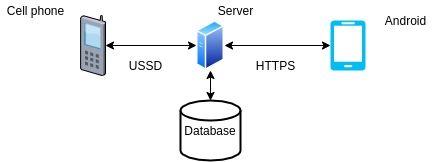
\includegraphics[width=1\linewidth]{figs/SA2.png}
\caption{Software Architecture for a proof of concept covering USSD and internet transactions through an android application.}
\label{fig: sa}
\end{figure}

As this is simply a proof of concept, the product is implemented with the English language in mind. If this product is to be tested on Guineans, the french language should at minimum be covered. Ideally with user settings to choose from the three other major languages spoken in Guinea.
\subsection{Server} % (fold)
We have implemented a C\# HTTP server that allows for multiple asynchronous connections at a time. This server supports the default operations of GET, PUT, PATCH, POST, DELETE. The server has the features mentioned earlier implemented.

The source code for the server is available in appendix B.1 and B.2.

\subsubsection{Database}
For simplicity, we have created an in-memory database. This database consists of three tables, the user table with the database schematic available in \autoref{tab: user}, the transaction table, with schematics available in \autoref{tab: transaction}, and the question table, with schematics available in \autoref{tab: question}. Since the database is stored as a global variable, it reduces the potential for a modular structure as all instructions would have to get and set the global variable from a different class with each call, whereas a relational database can be read from disk and updated through a simple query. Therefore the implementation has been done with the speed of implementation in mind, and not following design patterns such as MVC, MVP, or MVVM.

\begin{table}[ht]
\centering
\begin{tabular}{ll}
\hline
\multicolumn{2}{|c|}{\textbf{User}}                           \\ \hline
\multicolumn{1}{|l|}{\textbf{Column}}          & \multicolumn{1}{l|}{\textbf{Data type}} \\ \hline
\multicolumn{1}{|l|}{ID}        & \multicolumn{1}{l|}{Integer} \\ \hline
\multicolumn{1}{|l|}{Phone number}    & \multicolumn{1}{l|}{Integer} \\ \hline
\multicolumn{1}{|l|}{ActiveAgentEMoney} & \multicolumn{1}{l|}{Boolean} \\ \hline
\multicolumn{1}{|l|}{ActiveAgentCash}   & \multicolumn{1}{l|}{Boolean} \\ \hline
\multicolumn{1}{|l|}{EMoneyFee}     & \multicolumn{1}{l|}{Decimal} \\ \hline
\multicolumn{1}{|l|}{CashFee}       & \multicolumn{1}{l|}{Decimal} \\ \hline
\multicolumn{1}{|l|}{MaxAmountEMoney}   & \multicolumn{1}{l|}{Decimal} \\ \hline
\multicolumn{1}{|l|}{MaxAmountCash}   & \multicolumn{1}{l|}{Decimal} \\ \hline
\multicolumn{1}{|l|}{Pin}         & \multicolumn{1}{l|}{Integer} \\ \hline
\end{tabular}
\caption{The database schematic for the user.}
\label{tab: user}
\end{table}

\begin{table}[ht]
\centering
\begin{tabular}{ll}
\hline
\multicolumn{2}{|c|}{\textbf{Transaction}}                           \\ \hline
\multicolumn{1}{|l|}{\textbf{Column}}& \multicolumn{1}{l|}{\textbf{Data type}} \\ \hline
\multicolumn{1}{|l|}{ID}       & \multicolumn{1}{l|}{Integer} \\ \hline
\multicolumn{1}{|l|}{From (User\_ID)} & \multicolumn{1}{l|}{Integer} \\ \hline
\multicolumn{1}{|l|}{To (User\_ID)}   & \multicolumn{1}{l|}{Integer} \\ \hline
\multicolumn{1}{|l|}{Amount}     & \multicolumn{1}{l|}{Decimal} \\ \hline
\multicolumn{1}{|l|}{Fee}      & \multicolumn{1}{l|}{Decimal} \\ \hline
\multicolumn{1}{|l|}{Type}       & \multicolumn{1}{l|}{String} \\ \hline
\multicolumn{1}{|l|}{Status}     & \multicolumn{1}{l|}{String} \\ \hline
\multicolumn{1}{|l|}{Reason}     & \multicolumn{1}{l|}{String} \\ \hline
\multicolumn{1}{|l|}{Complete\_time}  & \multicolumn{1}{l|}{DateTime} \\ \hline
\end{tabular}
\caption{The database schematic for a transaction.}
\label{tab: transaction}
\end{table}

\begin{table}[ht]
\centering
\begin{tabular}{ll}
\hline
\multicolumn{2}{|c|}{\textbf{Question}}                           \\ \hline
\multicolumn{1}{|l|}{\textbf{Column}}& \multicolumn{1}{l|}{\textbf{Data type}} \\ \hline
\multicolumn{1}{|l|}{ID}       & \multicolumn{1}{l|}{Integer} \\ \hline
\multicolumn{1}{|l|}{From (User\_ID)} & \multicolumn{1}{l|}{Integer} \\ \hline
\multicolumn{1}{|l|}{Q}   & \multicolumn{1}{l|}{String} \\ \hline
\multicolumn{1}{|l|}{Asked\_time}  & \multicolumn{1}{l|}{DateTime} \\ \hline
\end{tabular}
\caption{The database schematic for a question.}
\label{tab: question}
\end{table}

\subsubsection{USSD API}
A USSD request is sent by the mobile network operator as a POST request with the following parameters:
\begin{itemize}
  \item \textbf{network code}

  This won't be relevant as we only operate on a single network.

  \item \textbf{phone number}

  The phone number of the user starting the USSD session

  \item \textbf{service code}

  The code the user has to call to start the USSD session

  \item \textbf{text} or \textbf{input}

  The input the user has entered, each step of the process separated with \textbf{*}. It's a text when it only includes integers, otherwise, it is parsed as an input. A text could look as such: \textit{11*15*5}, and input could look as such: \textit{1*please help me transfer money}.

  \item \textbf{session id}

  The unique id of the session created when the user called the USSD service code.
\end{itemize}

When developing to support USSD we will mainly utilize the phone number and the text. When a user connects to the USSD protocol, they need to be met with a list of possible actions. As such, when the \textit{text} string is empty, we return the following list in string format, such that dumbphones can parse it:
\begin{lstlisting}
"1 - Help \n"+
"2 - Check balance \n"+
"3 - List transactions \n" +
"4 - Transfer money \n"+
"5 - Request money \n"+
"6 - Deposit money \n"+
"7 - Withdraw money \n"+
"8 - Confirm transfer \n"+
"9 - Decline transfer \n"+
"10 - Deliver e-money \n"+
"11 - Deliver cash \n"+
"12 - Sign up"
\end{lstlisting}

By parsing the text input and splitting the inputs we can map the first input to an action on the list. From here we can either continue the process by returning \textit{"CON"} followed by the description of the next page. Otherwise, we use \textit{"END"} followed by the result of their action, e.g. their balance. For each input required by the user, a new description is required. From \autoref{fig: server_transfer} we can see a complete USSD request for a transfer. If the input in the request is valid and parsable, i.e. the amount of a transfer is greater than 0, the recipient exists, etc. The transaction occurs.

\begin{figure}[ht]
\centering
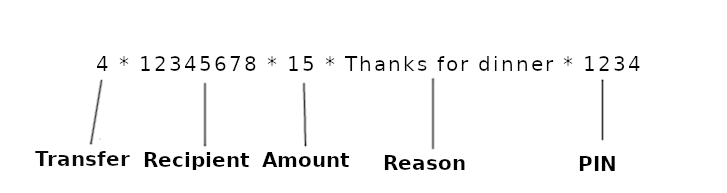
\includegraphics[width=1\linewidth]{figs/transfer_desc.png}
\caption{The input variables and their meaning of a complete USSD request}
\label{fig: server_transfer}
\end{figure}

After a request, deposit, or a withdrawal has been started, the agent should receive a notification, this can be implemented easily, either through an SMS, a network-initiated USSD or through an android notification. Currently a notification will be given from the terminal, as it requires a third-party service, such as a phone number to send text messages from.



\subsubsection{Android API}
To support the android application we utilize the same HTTP server, but with a different set of endpoints. Where each USSD request is sent to the same endpoint, reducing the possibility of modularity, we control the endpoints from the client-side of the android application. In total we list the following 15 endpoints:

\begin{itemize}
  \item POST /android/login
  \item POST /android/register
  \item POST /android/send (transfer)
  \item POST /android/deposit
  \item POST /android/withdraw
  \item POST /android/confirm
  \item POST /android/decline
  \item POST /android/stopAgent
  \item POST /android/becomeAgent
  \item POST /android/help
  \item POST /android/request
  \item GET /android/balance
  \item GET /android/agentstatus
  \item GET /android/history
  \item GET /android/agents
\end{itemize}

This differs slightly from the USSD implementation. USSD creates a session automatically, because the phone number is sent with the request, the android application will instead have to retrieve the phone number through a login system, thereby creating a user session in which the phone number of the user is known.

% subsection server (end)
\subsection{Android}
The android application has been implemented on API level 16, ensuring that over 99.8\% of all android devices are supported\footnote{99.8\% is a statistic mentioned by Android Studio upon creation of a project}. This is a minor concern since most of the phones in Africa uses android 10.0, 9.0 (Pie), or 8.1 (Oreo)\footnote{\url{https://gs.statcounter.com/android-version-market-share/mobile-tablet/africa} - Visited 2021-05-30}, which are all level 26 or higher.

The application has been made to ensure simplicity for the illiterate users of Guinea. All the different pages of the application can be seen in appendix A. Particularly, we would like to highlight the menu the user is met with after logging in, in appendix A.3, to point out how we accommodate these users. The design for this application was inspired by \textit{One app} by RedRose\footnote{\url{https://www.redrosecps.com/one-app.html} - Visited 2021-05-30}. Through the use of colors and icons, the ones with literacy issues can quickly become familiar with the application without risking their funds experimenting with the product.

The source code for all the pages and designs of the application is available in appendix B.3.

% subsection android (end)

\section{Evaluation}
We evaluate the implementation based on its use cases, performance, availability, attack vectors, and testing of the product.
\subsection{Use cases} % (fold)
\label{sub:use_cases}
This implementation has been tailor-made to support the population of Guinea, now, and in the future. As such, its main use case is to allow for banking through dumbphones, and smartphones to the Guineans. The use-cases include banking, transferring of money, as well as job opportunities for some of the poorest people in the world. We hope to employ additional use cases such as paying bills, day-to-day payments, as well as paying for airtime.

The model we have designed is not limited to the Guinean market, however, before deploying it to other markets, their specific needs would need to be accounted for. This is an agent-based model
as such it functions better in the dense urban regions of a country.

% subsection use_cases (end)
\subsection{Performance} % (fold)
\label{sub:performance}
The entirety of the banking system is automated, with all transactions settled close to immediately. It has been implemented with speed in mind, which is the reason for the choice of language, C\#.

% subsection performance (end)
\subsection{Availability} % (fold)
\label{sub:availability}
Availability is an important factor in a banking system. To ensure high uptime, every input, for all the endpoints is checked to ensure the existence and validity of the request to increase fault tolerance. The system is asynchronous and allows for multiple users at a time. To increase fault tolerance, it is possible to host multiple servers.

% subsection availability (end)
\subsection{Security} % (fold)
\label{sub:attack_vectors}
Banks are prone to attacks, whether the attacks are through physical means such as bank robberies, or hacking attempts. We list some of the known attack vectors and how we mitigate them, or how we are prone to them.

\begin{itemize}
  \item \textbf{Distributed Denial-of-Service (DDoS)}

  No actions have been taken to mitigate DDoS attacks, we mention it as it is important to mitigate such attacks to keep the system available at all times.
  \item \textbf{Social engineering}

  A typical attack vector is what is known as a SIM swap. It is the malicious act of convincing a users mobile network operator to swap their phone number. We mitigate such attacks by requiring confirmation before each action involving the transferring of money. The confirmation involves entering their PIN code.
  \item \textbf{Mobile network operators}

  While USSD is encrypted, the mobile network operator has free access to read all messages. This is a limitation of utilizing phones, whether this will remain a privacy concern, or an operator will use this information for their benefit is difficult to predict. Luckily HTTPS is encrypted, ensuring sniffing is not a problem in the future.
  \item \textbf{Replay attack}

  While there are other attack vectors, the last one we would like to highlight is known as a replay attack. It is the replay of an action. e.g. the confirmation of a transfer.

  The USSD mitigate this by automatically creating session ids, ensuring that all actions are performed from the same session, we have implemented a similar session system for the android part.

  Any confirmation of a transfer requires the use of a transaction id, when the status of the transaction with said id occurs, the status changes, ensuring that only a transfer of type "pending" can happen. As the id is unique to the transaction, no replayability is possible.
\end{itemize}

% subsection security_measures (end)

\subsection{Testing} % (fold)
\label{sub:testing}
Unit testing of the product has been done on all actions revolving around the transfer of money to ensure correctness. Further testing, as well as formal proof of correctness, which we will mention in future work, is in order.

\section{Discussion}
\subsection{Related work} % (fold)
\label{sub:related_work}

Money has been defined to have three functions: first, it should act as a medium of exchange; Second, it should represent a store of value; third, it should serve as a unit of account.\cite{carruthers}. The usage of money and the existance of banks have been known for centuries, however with technological advancements in the last decades, modern banking options have started to appear, and traditional banks have been required to digitize.

As the world is about to celebrate another millennium, wireless technology is booming. Back in 1999, Birch\cite{Birch1999MobileFS} sees this as a large opportunity for banks to expand on their services, by providing it through SMS anytime and anywhere. Tiwari \& Buse\cite{tiwaribuse} further define mobile banking in 2006 as the provision and availment of banking and financial services with the help of telecommunication devices. The services provided might include the ability to conduct bank and stock market transactions, administer bank accounts, or access customized information.

Since its appearance in 1999, mobile banking had yet to have any success. Khan\cite{khan} reports in 2008, that the early mobile banking attempts had suffered from slow speeds, lack of standardization, and anemic consumer adoption, but even after speed and device issues had been addressed, the interest in mobile banking wasn't there. Most consumers felt that transactions weren't urgent enough to warrant access through a mobile device. It wasn't until the success of Vodafone Groups M-Pesa in 2007\cite{jacksuri} that the world realized the potential that utilizing mobile devices to allow for banking opportunities could lead to a major positive impact on the least developed countries, as well as a major business opportunity.


% subsection related_work (end)
\subsection{Future work} % (fold)
\label{sub:future_work}

% subsection future_work (end)
\subsubsection{Field testing of the product} % (fold)
\label{sub:field_testing_of_the_product}
To ensure that all requirements of Guinea have been determined, it would be natural to test the implementation on a small group of people in Guinea. Gathering feedback and determining what could be improved upon before releasing the product is the logical next step in prototyping.
% subsection field_testing_of_the_product (end)

\subsubsection{Reservation} % (fold)
\label{sub:reservation}
The implementation for requests, withdrawals, and deposits currently works in 3 stages.
\begin{enumerate}
  \item A request is made for one person to send money to the other.
  \item the requested person and the requesting person meet and trades the cash.
  \item The requested person confirms the request in 1.
\end{enumerate}
This implementation does not take into account whether the requestee has the funds to finish the transfer. A reservation would be in order to prove that there is a sufficient amount of funds, thereby reducing theft opportunities.
% subsubsection pre_commit (end)

\subsubsection{Escrow service}
To reduce theft opportunities even further, a neutral escrow service, providing their service for a minor fee could be an interesting use case. Particularly for larger transactions.

\subsubsection{Blockchain / Distributed Ledger technology} % (fold)

\label{sub:blockchain_technology}

Obtaining an e-money license can be a long, tedious, and expensive process. As such, due to the unregulated nature of cryptocurrency, it might be easier to work with cryptocurrencies instead. There are additional benefits to this.
\begin{enumerate}
  \item Stablecoins are a type of cryptocurrency, typically pegged to the US Dollar. Utilizing stablecoins can allow for people in fluctuating economies to enter a stable one.
  \item Cryptocurrency is currently a popular means of investing and is being sought by multiple people. This allows for an additional business opportunity.
  \item Cryptocurrencies allow for easy cross-border transfers.
  \item No single point of failure as the data on a distributed ledger is shared between multiple nodes.
\end{enumerate}
The drawbacks however include an increase in fees to countervail the transaction fees of the network, as well as the unknown future and regulations of cryptocurrency.

\subsubsection{Formal proof} % (fold)
\label{sub:formal_proof}
Due to the sensitivity that is developing systems involving money, formally proving the implementation using a formal proof management system such as Coq\footnote{\url{https://coq.inria.fr/} - Visited 2021-05-30} would be in order, to further ensure correctness, thereby increasing trust.
% subsection subsection_name (end)

\section{Conclusion}
We have reasoned for the need for banking in the least developed countries. We further narrowed our scope to Guinea, a country with the infrastructure to support current mobile money implementations, and with a future of smartphones to come. We reasoned that there were some flaws in the existing mobile banking systems of Orange Money, MTN Mobile Money, and M-Pesa, and reasoned for a new model. We conclude that the simple modification of the M-Pesa model of changing the agent from local business to the average Joe, makes up for some of these flaws by converting from a static model to a dynamic model. By design, distance problems are reduced. Fee costs might be reduced, the service might even be free. Job opportunities are made for the average person willing to be the counterpart of exchanges, and lastly, the lack of identification no longer has to be a limiting factor to enter the banking world.

As the technology available in the least developed countries mainly consists of dumbphones, which by design has some flaws, such as the lack of privacy from mobile network operators. We recognize that a dumbphone cannot meet all the necessities of an ideal banking application, and therefore also propose an android application that utilizes HTTPS instead of USSD. This further allows for a better user experience than what simple texts can provide, covering the need for a non-text-based system for illiterat users. Utilizing android applications appear to be a given as the digital divide lessens. This also opens up for e-commerce and m-commerce, truly modernizing these countries.

\clearpage
\begingroup
\let\cleardoublepage\clearpage
\addcontentsline{toc}{section}{References}
\bibliographystyle{unsrt}
\bibliography{thesis}
\endgroup
\clearpage
\begin{appendices}

\section{Android application}

\subsection{Login page} % (fold)
\begin{figure}[ht]
\centering
\fbox{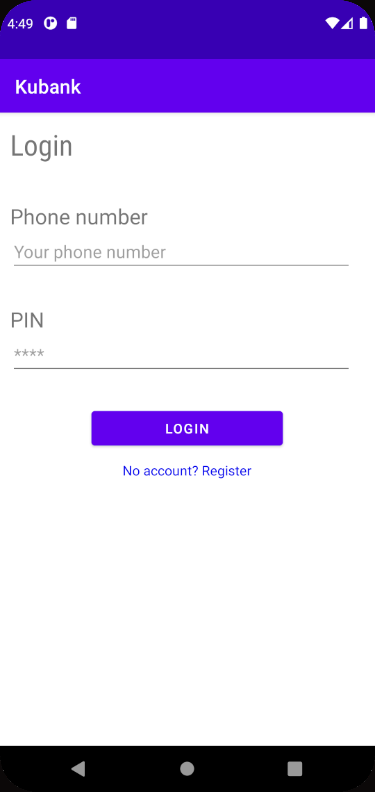
\includegraphics[width=0.55\linewidth]{figs/login}}
\caption{The login page of the android application}
\end{figure}
\clearpage

\subsection{Register page} % (fold)
\begin{figure}[ht]
\centering
\fbox{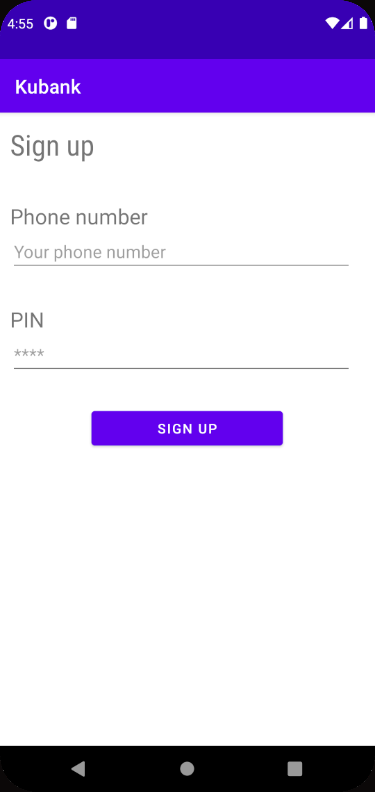
\includegraphics[width=0.55\linewidth]{figs/register}}
\caption{The register page of the android application}
\end{figure}
\clearpage
% subsection register_page (end)

% subsection login (end)
\subsection{Menu page} % (fold)
\begin{figure}[ht]
\centering
\fbox{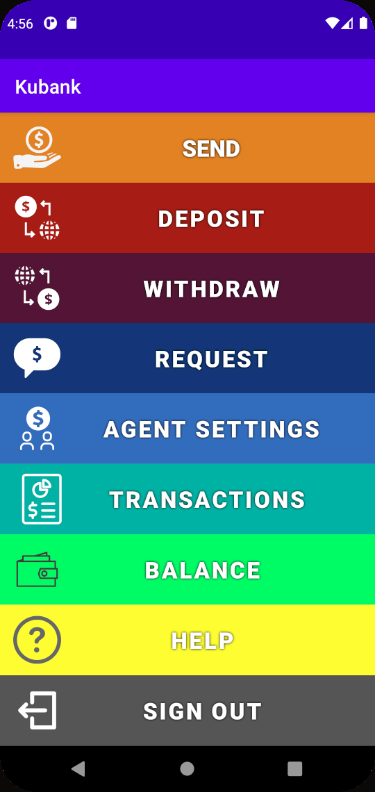
\includegraphics[width=0.55\linewidth]{figs/user}}
\caption{The menu page of the android application}
\end{figure}
\clearpage
% subsection menu_page (end)

\subsection{Transfer page} % (fold)
\begin{figure}[ht]
  \centering
  \begin{minipage}[b]{0.45\textwidth}
    \fbox{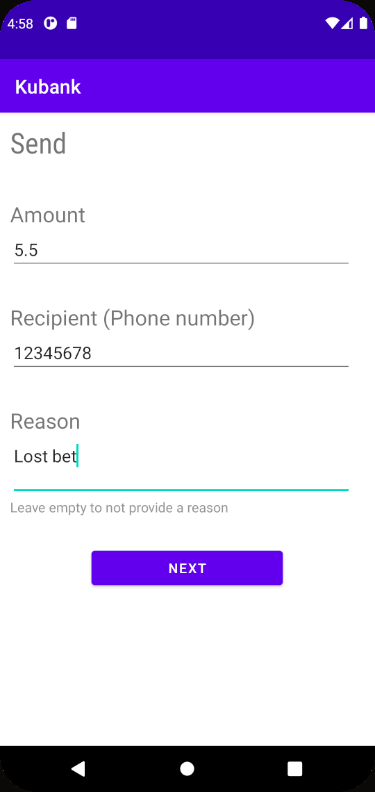
\includegraphics[width=\textwidth]{figs/send}}
    \caption{Step 1 of the send money flow of the android applicaton}
  \end{minipage}
  \hfill
  \begin{minipage}[b]{0.45\textwidth}
    \fbox{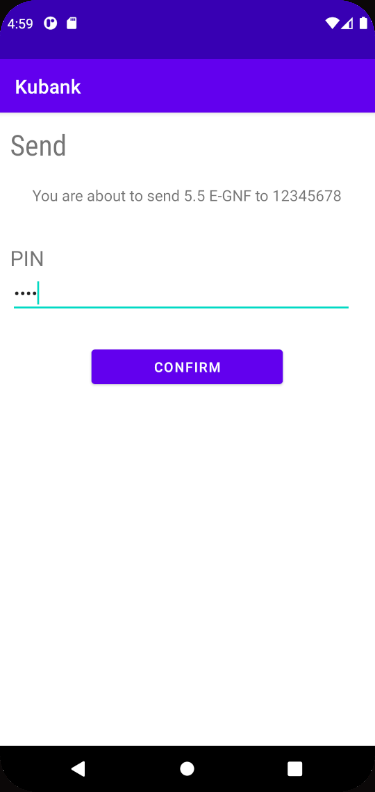
\includegraphics[width=\textwidth]{figs/send2}}
    \caption{Step 2 of the send money flow of the android applicaton}
  \end{minipage}
\end{figure}
\clearpage
% subsection transfer_page (end)

\subsection{Deposit page} % (fold)
\begin{figure}[ht]
  \centering
  \begin{minipage}[t]{0.45\textwidth}
    \fbox{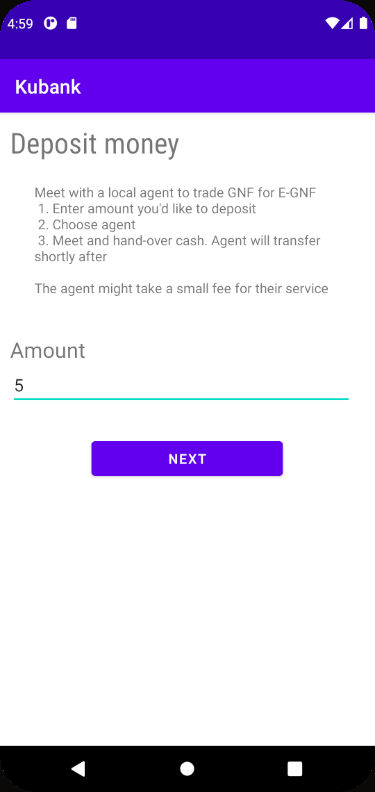
\includegraphics[width=\textwidth]{figs/deposit}}
    \caption{Step 1 of the deposit money flow of the android application}
  \end{minipage}
  \hfill
  \begin{minipage}[t]{0.45\textwidth}
    \fbox{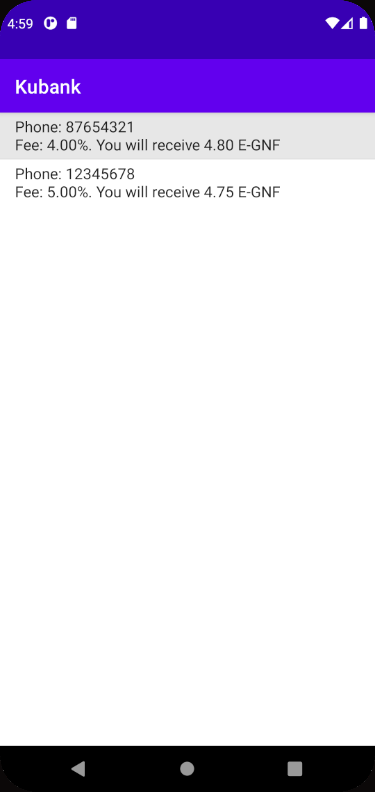
\includegraphics[width=\textwidth]{figs/deposit2}}
    \caption{Step 2 of the deposit money flow of the android application}
  \end{minipage}
\end{figure}

\begin{figure}[ht]
\centering
\fbox{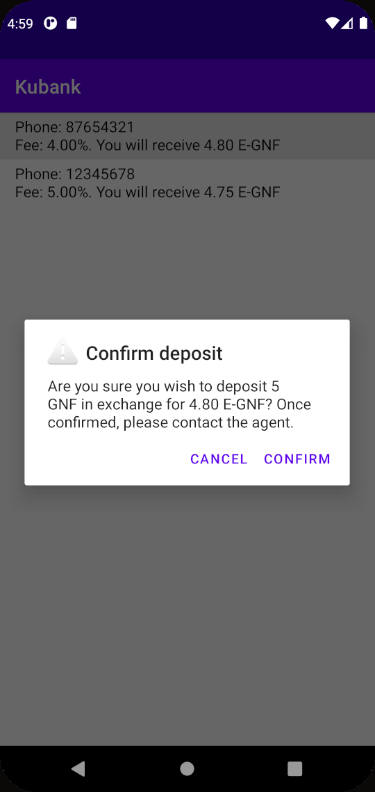
\includegraphics[width=0.55\linewidth]{figs/deposit3}}
\caption{Step 3 of the deposit money flow of the android application}
\end{figure}

\clearpage


% subsection deposit_page (end)
\subsection{Withdraw page} % (fold)
\begin{figure}[ht]
  \centering
  \begin{minipage}[t]{0.45\textwidth}
    \fbox{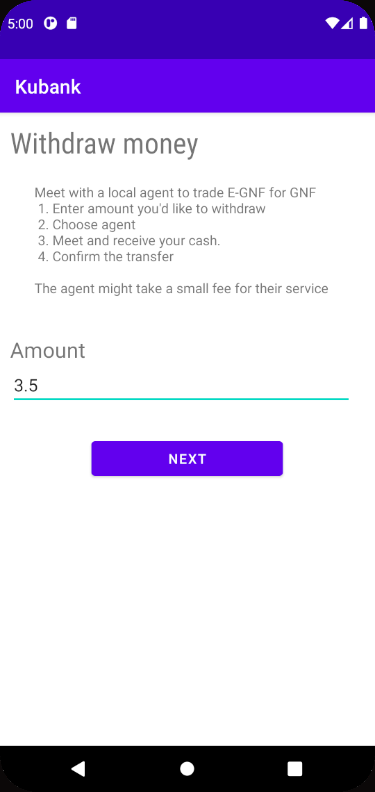
\includegraphics[width=\textwidth]{figs/withdraw}}
    \caption{Step 1 of the withdraw money flow of the android application}
  \end{minipage}
  \hfill
  \begin{minipage}[t]{0.45\textwidth}
    \fbox{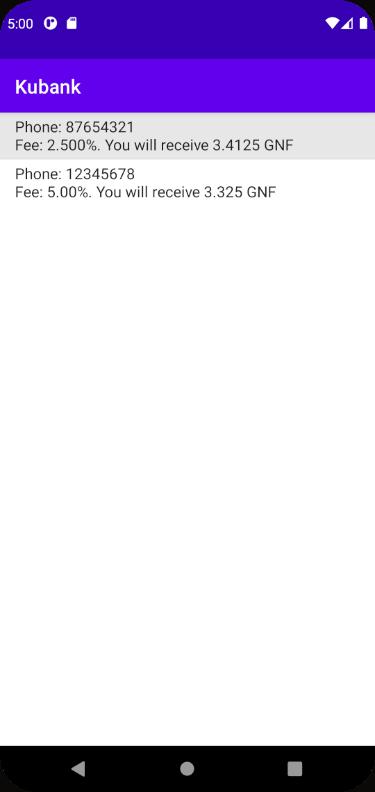
\includegraphics[width=\textwidth]{figs/withdraw2}}
    \caption{Step 2 of the withdraw money flow of the android application}
  \end{minipage}
\end{figure}

\begin{figure}[ht]
\centering
\fbox{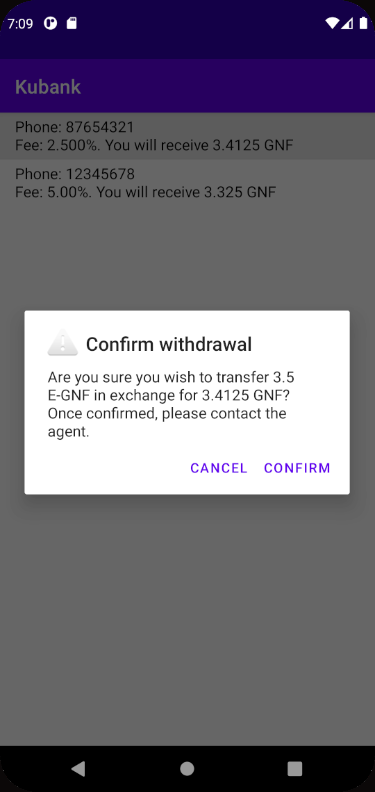
\includegraphics[width=0.55\linewidth]{figs/withdraw3.png}}
\caption{Step 3 of the withdraw money flow of the android application}
\end{figure}

\clearpage
% subsection withdraw_page (end)

\subsection{Request page} % (fold)
\begin{figure}[ht]
\centering
\fbox{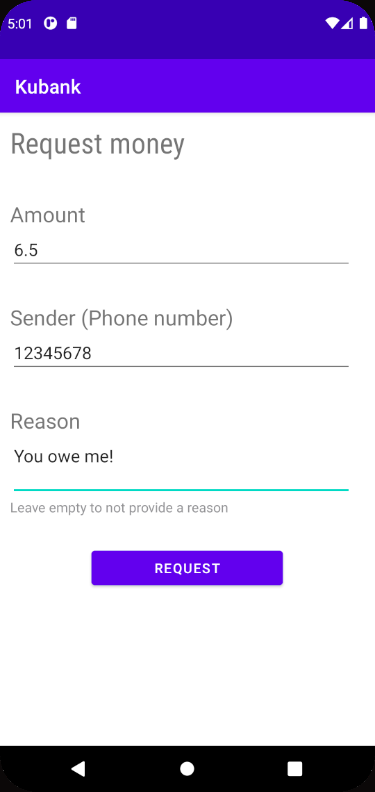
\includegraphics[width=0.55\linewidth]{figs/request}}
\caption{The request page of the android application}
\end{figure}
\clearpage

% subsection request_page (end)

\subsection{Transaction history page} % (fold)
\begin{figure}[ht]
\centering
\fbox{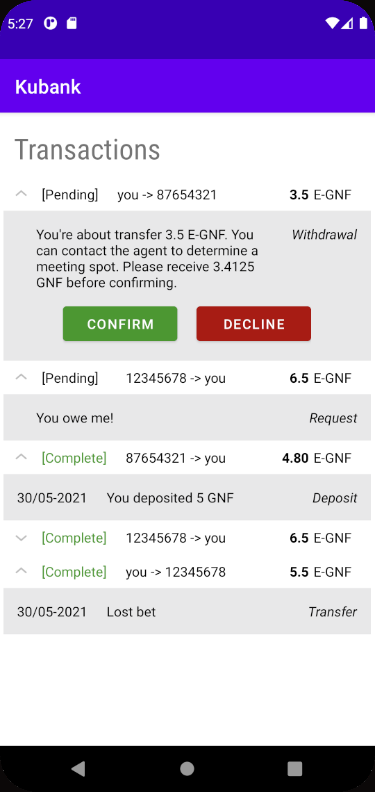
\includegraphics[width=0.55\linewidth]{figs/history}}
\caption{The history page of the android application}
\end{figure}
\clearpage

% subsection transaction_history_page (end)

\subsection{Agent settings page} % (fold)
\begin{figure}[ht]
\centering
\fbox{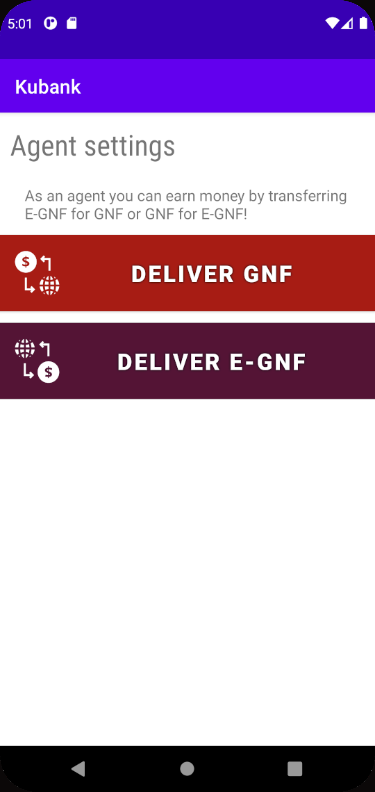
\includegraphics[width=0.55\linewidth]{figs/agent}}
\caption{The agent settings page of the android application}
\end{figure}
\clearpage

% subsection agent_settings_page (end)

\subsection{Agent deliver GNF page} % (fold)
\begin{figure}[ht]
\centering
\fbox{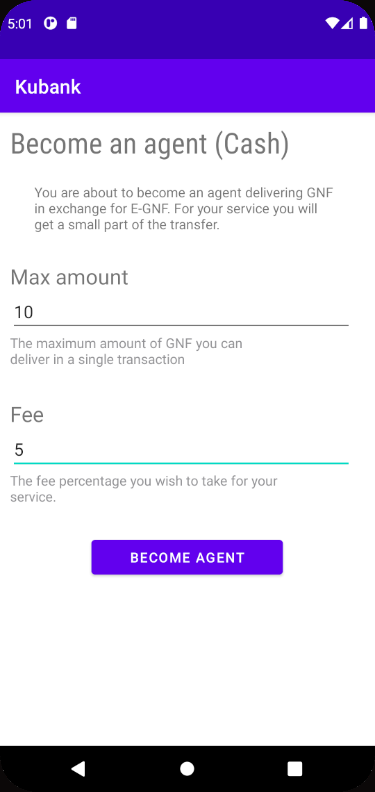
\includegraphics[width=0.55\linewidth]{figs/agentCash}}
\caption{The agent deliver GNF page of the android application}
\end{figure}
\clearpage

\subsection{Agent deliver E-GNF page} % (fold)
\begin{figure}[ht]
\centering
\fbox{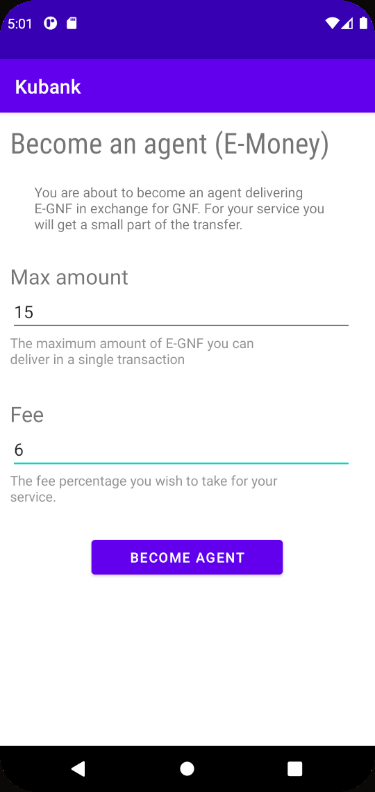
\includegraphics[width=0.55\linewidth]{figs/agentEmoney}}
\caption{The agent deliver E-GNF page of the android application}
\end{figure}
\clearpage

\subsection{Balance page} % (fold)
\begin{figure}[ht]
\centering
\fbox{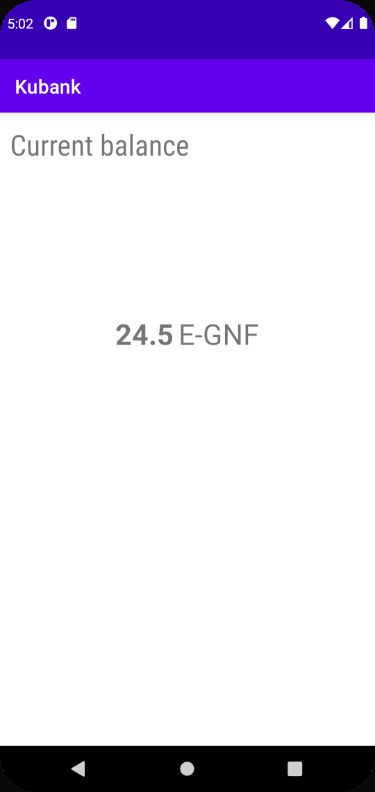
\includegraphics[width=0.55\linewidth]{figs/balance}}
\caption{The balance page of the android application}
\end{figure}
\clearpage

\subsection{Help page} % (fold)
\begin{figure}[ht]
\centering
\fbox{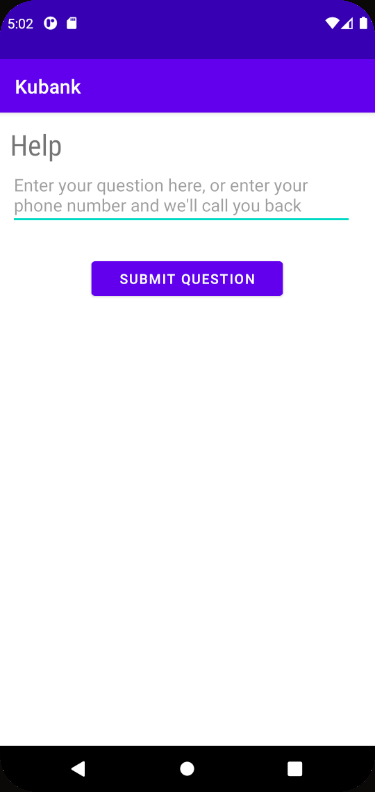
\includegraphics[width=0.55\linewidth]{figs/help}}
\caption{The help page of the android application}
\end{figure}
\clearpage

% subsection agent_settings_page_2 (end)

\section{Source code}
\subsection{Server} % (fold)
\label{sub:server}
\begin{lstlisting}
using System;
using System.IO;
using System.Text;
using System.Net;
using System.Threading.Tasks;
using System.Linq;
using System.Net.Mime;
using System.Collections.Generic;
using static System.Net.WebUtility;
using System.Text.Json;
using BankTypes;

namespace HttpListenerBank
{

 public static class LingExtension
 {
  public static IEnumerable<T> SetValue<T>(this IEnumerable<T> items, Action<T>updateMethod)
  {
   foreach (T item in items)
   {
  updateMethod(item);
   }
   return items;
  }
 }


 class HttpServer
 {
  public static HttpListener listener;
  public static string port = System.Environment.GetEnvironmentVariable("PORT");
  public static int pageViews = 0;
  public static bool showRequestInfo = false;
  public static int requestCount = 0;
  public static string pageData =
   "<html>" +
   "  <head>" +
   " <style> " +
   "   table {{border-collapse: collapse}}" +
   "   table {{min-width: 1000px;}}" +
   " table tr td {{border: solid 1px #C7C7C7;}}" +
   " </style>" +
   "  </head>" +
   "  <body>" +
   " {0}" + // account table
   " <br/><br/>"+
   " {1}" + // transaction table
   " <br/><br/>"+
   " {2}" + // question table
   " <br/><br/><br/>" +
   " <form method=\"post\" action=\"reset\">" +
   "   <input type=\"submit\" value=\"Reset\">" +
   " </form>" +
   " <form method=\"post\" action=\"donate\">" +
   "   <input type=\"submit\" value=\"donate 10 E-GNF to all users\">" +
   " </form>" +

   "  </body>" +
   "</html>";


  public static List<User> userList = new List<User>() {
  };

  public static List<Question> questionList = new List<Question>() {
  };

  public static List<Transaction> transactionList = new List<Transaction>() {
  };

  // token -> phone number
  public static Dictionary<string, int> usersLoggedIn = new Dictionary<string, int>(){};


  private static void reset(){
   userList = new List<User>(){
//  new User() { ID = 1, PhoneNumber = 12345678, Balance = 100.0m, ActiveAgentEMoney = true, ActiveAgentCash = true, MaxAmountEMoney = 20, CashFee = 0.05m, EMoneyFee = 0.05m, MaxAmountCash = 25, Pin = 1234} ,
//  new User() { ID = 2, PhoneNumber = 87654321, Balance = 100.0m, ActiveAgentEMoney = true, ActiveAgentCash = true, MaxAmountEMoney = 200, CashFee = 0.1m, EMoneyFee = 0.1m, MaxAmountCash = 200,  Pin = 1234} ,
   };
   transactionList = new List<Transaction>() {
  // new Transaction() { ID = 1, From = 1, To = 2, Amount = (decimal) 5m, Fee = (decimal) 1.0m, Type = "Deposit", Status = "Complete", Reason = null, Complete_time = DateTime.Now } // User 1 has deposited 5 GNF through User 2. In return user 1 has received 4.95 E-GNF
   };

   questionList = new List<Question>(){};

   usersLoggedIn = new Dictionary<string, int>(){};
  }



  private static (int, string) Confirm(int PhoneNumber, int id, int pin){
   // Find user id
   User user = userList.SingleOrDefault(u => u.PhoneNumber == PhoneNumber);
   if(user == null){
  return (-1, "No user with that phonenumber found");
   }
   // Check if correct pin
   if(user.Pin != pin){
  return (-1, "Incorrect pin code");
   }

   // Fetch transaction
   try{
  Transaction transaction = transactionList.SingleOrDefault(t => t.From == user.ID && t.Status == "Pending" && t.ID == id);
  decimal toTransfer = 0m;
  if (transaction.Type == "Withdrawal"){
   toTransfer = transaction.Amount;
  } else{
   toTransfer = transaction.Amount - transaction.Amount * transaction.Fee;
  }
  if(user.Balance < toTransfer){
   return (-1, "Invalid funds available to complete transfer");
  }


  // Do transfer
  // Not ACID-proof but for a concept it should be fine
  if (transaction.Type == "Withdrawal"){
   // A user would like to withdraw 10 E-GNF worth cash. In order to do so he transfers 10 E-GNF and in return gets 10-10*fee GNF in cash
   userList.Where(u => u.ID == transaction.From).SetValue(u => u.Balance = u.Balance - transaction.Amount);
   userList.Where(u => u.ID == transaction.To).SetValue(u => u.Balance = u.Balance + transaction.Amount);
  } else{
   userList.Where(u => u.ID == transaction.From).SetValue(u => u.Balance = u.Balance - toTransfer);
   userList.Where(u => u.ID == transaction.To).SetValue(u => u.Balance = u.Balance + toTransfer);
  }

  // Update order to complete
  transactionList.Where(t => t.ID == transaction.ID).SetValue(t => t.Status = "Complete").SetValue(t => t.Complete_time = DateTime.Now);

  // Notify sender and recipient that they have confirmed the transaction
  User from = userList.SingleOrDefault(u => u.PhoneNumber == transaction.From);
  User to = userList.SingleOrDefault(u => u.PhoneNumber == transaction.To);
  if(from != null && to != null){
   var retSender = "";
   var retRecipient = "";

   if(transaction.Type == "Transfer"){
    // Send to sender
    retSender = $"SMS -> ({from.PhoneNumber}) You have sent {transaction.Amount} E-GNF to {to.PhoneNumber}";
    if(transaction.Reason != null){
     retSender+=$". \" {transaction.Reason} \"";
    }

    // Send to recipient
    retRecipient = $"SMS -> ({to.PhoneNumber}) You have received {transaction.Amount} E-GNF from {from.PhoneNumber}";
    if(transaction.Reason != null){
     retRecipient+=$". \" {transaction.Reason} \"";
    }
   }
   else if(transaction.Type == "Request"){
    // Send to sender
    retSender = $"SMS -> ({from.PhoneNumber}) You have sent the requested {transaction.Amount} E-GNF to {to.PhoneNumber}";
    if(transaction.Reason != null){
     retSender+=$". \" {transaction.Reason} \"";
    }

    // Send to recipient
    retRecipient = $"SMS -> ({to.PhoneNumber}) You have received your requested {transaction.Amount} E-GNF from {from.PhoneNumber}";
    if(transaction.Reason != null){
     retRecipient+=$". \" {transaction.Reason} \"";
    }
   }
   else if (transaction.Type == "Deposit"){
    // Send to sender
    retSender = $"SMS -> ({from.PhoneNumber}) You have delivered {transaction.Amount - (transaction.Amount*transaction.Fee)} E-GNF to {to.PhoneNumber} in exchange for {transaction.Amount} GNF";
    // Send to recipient
    retRecipient = $"SMS -> ({to.PhoneNumber}) You have deposited {transaction.Amount} GNF through {from.PhoneNumber}. Your account balance has increased by {transaction.Amount - (transaction.Amount*transaction.Fee)} E-GNF";
   } else if(transaction.Type == "Withdrawal"){
    // Send to sender (in this case, the sender is the user, the recipient is the agent)
    retSender = $"SMS -> ({from.PhoneNumber}) You have withdrawed {transaction.Amount - (transaction.Amount*transaction.Fee)} GNF through {to.PhoneNumber} in exchange for {transaction.Amount} E-GNF";
    // Send to recipient
    retRecipient = $"SMS -> ({to.PhoneNumber}) You have delivered {transaction.Amount - (transaction.Amount*transaction.Fee)} GNF to {to.PhoneNumber} in exchange for {transaction.Amount} E-GNF";
   }
   Console.WriteLine(retSender);
   Console.WriteLine(retRecipient);
  }



  return (0, "Success");
   } catch(Exception e){
  Console.WriteLine(e);
  return (-1, "Operation failed");
   }

  }

  private static (int, string) Decline(int PhoneNumber, int id){
   User user = userList.SingleOrDefault(u => u.PhoneNumber == PhoneNumber);
   if(user == null){
  return (-1, "No user with that phonenumber found");
   }
   // Fetch transaction
   transactionList.Where(t => t.From == user.ID && t.Status == "Pending" && t.ID == id).SetValue(t => t.Complete_time = DateTime.Now).SetValue(t => t.Status = "Declined");
   return (0, "");

  }

  private static (int, decimal) GetBalance(int PhoneNumber){
   User user = userList.SingleOrDefault(u => u.PhoneNumber == PhoneNumber);
   if(user == null){
  return (-1, 0m);
   }
   else {
  return (0, user.Balance);
   }
  }

  private static (int, List<DTransaction>) ListTransactions(int PhoneNumber, int offset, int amount){
   try{
  User user = userList.SingleOrDefault(u => u.PhoneNumber == PhoneNumber);
  List<Transaction> ts = transactionList.Where(t => t.From == user.ID || t.To == user.ID).OrderByDescending(t => t.Status == "Pending").ThenByDescending(t => t.Complete_time).ToList();
  ts = ts.Skip(offset).Take(amount).ToList();
  List<DTransaction> newts = new List<DTransaction>();
  Dictionary<int, string> dp = new Dictionary<int, string>(); // convert user ids to phone number
  foreach(Transaction t in ts){
   DTransaction newT = new DTransaction() {ID = t.ID, From = null, To = null, Amount = t.Amount, Fee = t.Fee, Type = t.Type, Status = t.Status, Reason=t.Reason, Complete_time = t.Complete_time};
   // convert from ids to phone numbers
   if (t.From == user.ID){
    newT.From = "you";
   } else{
    if(dp.ContainsKey(t.From)){
     newT.From = dp[t.From];
    } else{
     User u = userList.SingleOrDefault(u => u.ID == t.From);
     if(u == null){
    Console.WriteLine($"Tried converting ID to phonenumber for user ID {t.From} but it failed");
     } else{
    dp.Add(t.From, u.PhoneNumber.ToString());
    newT.From = u.PhoneNumber.ToString();
     }

    }
   }


   // convert to ids to phone numbers
   if (t.To == user.ID){
    newT.To = "you";
   } else{
    if(dp.ContainsKey(t.To)){
     newT.To = dp[t.To];
    } else{
     User u = userList.SingleOrDefault(u => u.ID == t.To);
     if(u == null){
    Console.WriteLine($"Tried converting ID to phonenumber for user ID {t.To} but it failed");
     } else{
    dp.Add(t.To, u.PhoneNumber.ToString());
    newT.To = u.PhoneNumber.ToString();
     }

    }
   }

   newts.Add(newT);
  }
  return (newts.Count, newts);
   } catch(Exception e){
  Console.WriteLine(e);
  return (-1, null);
   }
  }

  private static (int, string) Transfer(int fromphone, int tophone, decimal amount, decimal fee, string type, string reason){
   User from = userList.SingleOrDefault(u => u.PhoneNumber == fromphone);
   if(from == null){
  return (-1, "Sender not found");
   }
   User to = userList.SingleOrDefault(u => u.PhoneNumber == tophone);
   if(to == null){
  return (-1, "Recipient does not exist");
   }
   if(tophone == fromphone){
  return (-1, "Can't send E-GNF to yourself");
   }
   if(amount < 0.0m){
  return (-1, "Amount can't be negative");
   }
   if(amount < 0.1m){
  return (-1, "Amount can't be less than 0.1 E-GNF");
   }
   if(fee < 0.0m){
  return (-1, "Fee can't be negative");
   }

   int TCount = transactionList.Count;
   Transaction newT = new Transaction() {ID = TCount+1, From = from.ID, To = to.ID, Amount = amount, Fee = fee, Type = type, Status = "Pending", Reason=reason, Complete_time = DateTime.MinValue};
   try{
  transactionList.Add(newT);

  // Notify agent
  if (type == "Withdrawal"){
   // Should be an SMS
   Console.WriteLine($"SMS -> ({to.PhoneNumber}) - User {from.PhoneNumber} has requested {amount-amount*fee} GNF in exchange for {amount} E-GNF");
  } else if(type == "Deposit"){
   Console.WriteLine($"SMS -> ({from.PhoneNumber}) - User {to.PhoneNumber} has requested {amount-amount*fee} E-GNF in exchange for {amount} GNF");
  } else if(type == "Request"){
   string ret = $"SMS -> ({from.PhoneNumber}) - User {to.PhoneNumber} has requested {amount-amount*fee} E-GNF";
   if(reason != null && reason != ""){
    ret+=$". \" {reason} \"";
   }
   Console.WriteLine(ret);
  }
   } catch(Exception e){
  Console.WriteLine(e);
   }
   return (TCount+1, "");
  }

  // The agent marks themselves as available to transfer cash
  private static (int, string) SetAgentStatusCash(int Phonenumber, decimal MaxAmount, decimal fee){
   if(MaxAmount < 0.0m){
  return (-1, "Amount can't be negative");
   }
   if(fee < 0.0m){
  return (-1, "Fee can't be less than 0");
   }
   if(fee > 100.0m){
  return (-1, "Fee can't be greater than 100");
   }
   User user = userList.SingleOrDefault(u => u.PhoneNumber == Phonenumber);
   if(user == null){
  return (-1, "User not found");
   }

   userList.Where(u => u.ID == user.ID)
  .SetValue(u => u.ActiveAgentCash = !u.ActiveAgentCash)
  .SetValue(u => u.CashFee = fee/100.0m)
  .SetValue(u => u.MaxAmountCash = MaxAmount);
   return (0, "");
  }

  private static (int, string) SetAgentStatusEMoney(int Phonenumber, decimal MaxAmount, decimal fee){
   User user = userList.SingleOrDefault(u => u.PhoneNumber == Phonenumber);
   if(user == null){
  return (-1, "User not found");
   }

   userList.Where(u => u.ID == user.ID)
  .SetValue(u => u.ActiveAgentEMoney = !u.ActiveAgentEMoney)
  .SetValue(u => u.EMoneyFee = fee/100.0m)
  .SetValue(u => u.MaxAmountEMoney = MaxAmount);
   return (0, "");
  }

  private static int NewUser(int pin, int phone){
   try{
  User user = userList.SingleOrDefault(u => u.PhoneNumber == phone);
  if(user != null){
   return -1;
  } else{
   int UserCount = userList.Count;
   User newU = new User() {ID = UserCount+1, PhoneNumber = phone, Balance = 0, ActiveAgentEMoney = false, ActiveAgentCash = false, MaxAmountEMoney = 0, MaxAmountCash = 0, Pin = pin};
   userList.Add(newU);
   return 0;
  }
   } catch(Exception e){
  Console.WriteLine(e);
  return -1;
   }
  }

  private static (int, string) newQuestion(int phone, string question){

   User user = userList.SingleOrDefault(u => u.PhoneNumber == phone);
   if(user == null){
  return (-1, "Your phone number could not be found. Are you registered?");
   }
   int qCount = questionList.Count;
   Question newQ = new Question() {ID = qCount+1, From = user.ID, Q = question, Asked_time = DateTime.Now};
   questionList.Add(newQ);
   return (0, "Success");
  }

  private static void testTransfer(){
   // Transfer
   bool testTransfer = true;
   bool testRequest = true;
   bool testDeposit = true;
   bool testWithdraw = true;
   bool testDecline = true;

   if(testTransfer){
  var (id, _) = Transfer(12345678, 87654321, 5m, 0.00m, "Transfer", "For dinner tonight :)");
  var (_, balgiver) = GetBalance(12345678);
  var (_, balrecipient) = GetBalance(87654321);
  Confirm(12345678, id, 1234);
  decimal expectedGiver = balgiver - 5m;
  decimal expectedRecipient = balrecipient + 5m;
  var (_, balgiver2) = GetBalance(12345678);
  var (_, balrecipient2) = GetBalance(87654321);
  if (balrecipient2 == expectedRecipient && balgiver2 == expectedGiver){
   Console.WriteLine("Test (Transfer) - Passed");
  } else{
   Console.WriteLine("Test (Transfer) - Failed");
   Console.WriteLine($"Expected: {expectedRecipient} & {expectedGiver}");
   Console.WriteLine($"Got {balrecipient2} & {balgiver2}");
  }
   }

   if(testRequest){
  var (id, _) = Transfer(87654321, 12345678, 5m, 0.00m, "Request", "For dinner tonight :)");
  var (_, balrecipient) = GetBalance(12345678);
  var (_, balgiver) = GetBalance(87654321);
  Confirm(87654321, id, 1234);
  decimal expectedGiver = balgiver - 5m;
  decimal expectedRecipient = balrecipient + 5m;
  var (_, balgiver2) = GetBalance(87654321);
  var (_, balrecipient2) = GetBalance(12345678);
  if (balrecipient2 == expectedRecipient && balgiver2 == expectedGiver){
   Console.WriteLine("Test (Request) - Passed");
  } else{
   Console.WriteLine("Test (Request) - Failed");
   Console.WriteLine($"Expected: {expectedRecipient} & {expectedGiver}");
   Console.WriteLine($"Got {balrecipient2} & {balgiver2}");
  }
   }

   // Deposit
   if(testDeposit){
  decimal amount = 10m;
  decimal fee = 0.05m;
  var (b1, baluser) = GetBalance(12345678);
  var (b2, balagent) = GetBalance(87654321);
  var (id, _) = Transfer(87654321, 12345678, amount, fee, "Deposit", null);
  Confirm(87654321, id, 1234);
  var (b5, baldepositUser) = GetBalance(12345678);
  var (b6, baldepositAgent) = GetBalance(87654321);
  decimal expectedUser = baluser + (amount-(amount*fee));
  decimal expectedAgent = balagent - (amount-(amount*fee));
  if (baldepositAgent == expectedAgent && baldepositUser == expectedUser){
   Console.WriteLine("Test (Deposit) - Passed");
  } else{
   Console.WriteLine("Test (Deposit) - Failed");
   Console.WriteLine($"Expected: {expectedAgent} & {expectedUser}");
   Console.WriteLine($"Got {baldepositAgent} & {baldepositUser}");
  }
   }

   // Withdrawal
   if(testWithdraw){
  decimal amount = 10m;
  decimal fee = 0.05m;
  var (_, baluser) = GetBalance(12345678);
  var (_, balagent) = GetBalance(87654321);
  var (id, _) = Transfer(12345678, 87654321, amount, fee, "Withdrawal", null);
  Confirm(12345678, id, 1234);
  var (_, baldepositUser) = GetBalance(12345678);
  var (_, baldepositAgent) = GetBalance(87654321);
  decimal expectedUser = baluser - amount;
  decimal expectedAgent = balagent + amount;
  if (baldepositAgent == expectedAgent && baldepositUser == expectedUser){
   Console.WriteLine("Test (Withdrawal) - Passed");
  } else{
   Console.WriteLine("Test (Withdrawal) - Failed");
   Console.WriteLine($"Expected: {expectedAgent} & {expectedUser}");
   Console.WriteLine($"Got {baldepositAgent} & {baldepositUser}");
  }
   }

   if(testDecline){
  decimal amount = 10m;
  decimal fee = 0m;
  var (_, baluser) = GetBalance(12345678);
  var (_, balagent) = GetBalance(87654321);
  var (id, _) = Transfer(12345678, 87654321, amount, fee, "Transfer", "yay");
  Decline(12345678, id);
  var (_, baldepositUser) = GetBalance(12345678);
  var (_, baldepositAgent) = GetBalance(87654321);
  decimal expectedUser = baluser;
  decimal expectedAgent = balagent;
  if (baldepositAgent == expectedAgent && baldepositUser == expectedUser){
   Console.WriteLine("Test (Decline) - Passed");
  } else{
   Console.WriteLine("Test (Decline) - Failed");
   Console.WriteLine($"Expected: {expectedAgent} & {expectedUser}");
   Console.WriteLine($"Got {baldepositAgent} & {baldepositUser}");
  }
   }
  }

  private static string formatUserHtml(){
   string ret = "<h1>Users</h1>"+
   "<table id='uTable'>"+
   " <thead>"+
   "  <tr>"+
   "   <td><b>ID</b></td>"+
   "   <td><b>Phone number</b></td>"+
   "   <td><b>Balance</b></td>"+
   "   <td><b>Agent (cash)</b></td>"+
   "   <td><b>Agent fee (cash)</b></td>"+
   "   <td><b>Max amount (cash)</b></td>"+
   "   <td><b>Agent (E-money)</b></td>"+
   "   <td><b>Agent fee (E-money)</b></td>"+
   "   <td><b>Max amount (E-money)</b></td>"+
   "  </tr>"+
   "  </thead>"+
   "<tbody>";
   foreach (User user in userList){
  ret+=$"<tr>"+
   $"<td>{user.ID}</td>"+
   $"<td>{user.PhoneNumber}</td>"+
   $"<td>{user.Balance}</td>"+
   $"<td>{user.ActiveAgentCash}</td>"+
   $"<td>{user.CashFee}</td>"+
   $"<td>{user.MaxAmountCash}</td>"+
   $"<td>{user.ActiveAgentEMoney}</td>"+
   $"<td>{user.EMoneyFee}</td>"+
   $"<td>{user.MaxAmountEMoney}</td>"+
   "</tr>";
   }
   ret+="</tbody></table>";
   return ret;
  }
  private static string formatTransactionHtml(){
   string ret = "<h1>Transactions</h1><table id='tTable'><thead><tr>" +

   "<td><b>ID</b></td>" +
   "<td><b>From</b></td>" +
   "<td><b>To</b></td>"+
   "<td><b>Amount</b></td>"+
   "<td><b>Fee</b></td>"+
   "<td><b>Sent</b></td>"+
   "<td><b>Received</b></td>"+
   "<td><b>Reason</b></td>"+
   "<td><b>Type</b></td>"+
   "<td><b>Status</b></td>"+
   "<td><b>Complete time</b></td>"+

   "</tr></thead><tbody>";
   foreach (Transaction t in transactionList){
  decimal sent = t.Amount - t.Amount*t.Fee;
  decimal received = 0.00m;
  string sentstr = "";
  string recstr = "";
  if(t.Type == "Deposit"){
   sentstr = $"{(t.Amount - (t.Amount*t.Fee))} E-GNF";
   recstr = $"{t.Amount} GNF";
  } else if(t.Type == "Withdrawal"){
   sentstr = $"{t.Amount} E-GNF";
   recstr = $"{(t.Amount - (t.Amount*t.Fee))} GNF";
  } else{
   sentstr = $"{sent} E-GNF";
   recstr = $"{received} GNF";
  }

  ret+=$"<tr>"+

  $"<td>{t.ID}</td>"+
  $"<td>{t.From}</td>" +
  $"<td>{t.To}</td>" +
  $"<td>{t.Amount}</td>" +
  $"<td>{t.Fee}</td>" +
  $"<td>{sentstr}</td>" +
  $"<td>{recstr}</td>" +
  $"<td>{t.Reason}</td>" +
  $"<td>{t.Type}</td>" +
  $"<td>{t.Status}</td>" +
  $"<td>{t.Complete_time}</td>" +

  "</tr>";
   }
   ret+="</tbody></table>";
   return ret;
  }

  private static string formatQuestionHtml(){
   string ret = "<h1>Questions</h1><table id='tTable'><thead><tr>" +

   "<td><b>ID</b></td>" +
   "<td><b>From</b></td>" +
   "<td><b>Question</b></td>"+
   "<td><b>When asked</b></td>"+

   "</tr></thead><tbody>";
   foreach (Question q in questionList){
  ret+=$"<tr>"+

  $"<td>{q.ID}</td>"+
  $"<td>{q.From}</td>" +
  $"<td>{q.Q}</td>" +
  $"<td>{q.Asked_time}</td>" +

  "</tr>";
   }
   ret+="</tbody></table>";
   return ret;
  }
















  // USD
  public static string handleUSSD(Dictionary<String, String> data){

   string reqText = "";
   if(data.ContainsKey("text")){
  reqText = data["text"];
   } else if(data.ContainsKey("input")){
  reqText = data["input"];
   } else{
  return "END No form data could be found";
   }
   int reqPhone = int.Parse(data["phoneNumber"].Remove(0,3)); // remove +45 for danish numbers. Good enough for proof of concept
   string[] sections = reqText.Split('*');
   string section = sections[0];
   int reqlen = sections.Length;
   switch(section){
  case "
   string response = "CON "+
     "1 - Help \n"+
     "2 - Check balance \n"+
     "3 - List transactions \n" +
     "4 - Transfer money \n"+
     "5 - Request money \n"+
     "6 - Deposit money \n"+
     "7 - Withdraw money \n"+
     "8 - Confirm transfer \n"+
     "9 - Decline transfer \n"+
     "10 - Deliver e-money \n"+
     "11 - Deliver cash \n"+
     "12 - Sign up";
   return response;
  case "1 // help
   if(reqlen == 1){
    return "CON enter a question and we'll get back to you. If you'd like for us to call you, leave this space empty";
   } else{
    var (err, msg) = newQuestion(reqPhone, sections[1]);
    if(err == -1) {
     return $"END {msg}";
    } else{
     return $"END Your question has been sent. You'll get a response shortly";
    }
   }
  case "2 // balance
  {
   var (err, bal) = GetBalance(reqPhone);
   if(err == 0){
    return $"END Your balance is: {bal.ToString()} E-GNF";
   } else{
    return $"END Something went wrong. Have you signed up?";
   }
  }
  case "3 // list transactions
   if(reqlen == 1){
    User user = userList.SingleOrDefault(u => u.PhoneNumber == reqPhone);
    if(user == null){
     return "END Your phone number could not be found. Are you registered?";
    }
    return "CON Please enter the order offset. 0 if you would like to see the 5 latest transactions. 5 if you'd like to see the 5 afterwards, 10 for the following 5 and so on.";
   } else{
    var (amount, ts) = ListTransactions(reqPhone, int.Parse(sections[1]), 5);
    if(amount == -1){
     return $"END Something went wrong. Have you signed up?";
    } else{
     if(amount == 0){
    return "END No transactions found";
     } else{
    string ret = "END "; //$"END {"From - To - Amount - Fee - Type"} \n";
    foreach(DTransaction t in ts){
     if(t.Complete_time != DateTime.MinValue){
      ret+=$"{t.Complete_time.ToString("dd-MM")} : ";
     }
     if(t.Type == "deposit"){
      ret+=$"{t.From} -> {t.To}. {t.Amount - t.Amount*t.Fee} E-GNF ({t.Type}) [{t.Status}]"; // 02-05 : you -> 12345678. 1.23 GNF (Transfer) [Completed] "Cinema"
     } else{
      ret+=$"{t.From} -> {t.To}. {t.Amount} E-GNF ({t.Type}) [{t.Status}]"; // 02-05 : you -> 12345678. 1.23 GNF (Transfer) [Completed] "Cinema"
     }
     if(t.Reason != null && t.Reason != ""){
      ret+=$" \"{t.Reason}\"";
     }
     ret+="\n";
    }
    return ret;
     }
    }
   }
  case "4 // transfer
   switch(reqlen){
    case 1:
     User user = userList.SingleOrDefault(u => u.PhoneNumber == reqPhone);
     if(user == null){
    return "END Your phone number could not be found. Are you registered?";
     }
     return "CON Please enter the phone number of the recipient";
    case 2:
     return $"CON Please enter the amount of E-GNF you'd like to send to {sections[1]}";
    case 3:
     return $"CON Please enter the reason for the transfer. e.g. dinner or bill. Enter 0 if you'd like to not provide a reason";
    case 4:
     return $"CON Please complete your transfer of {sections[2]} E-GNF to {sections[1]} by entering your PIN. Enter 0 to cancel";
    case 5:
     if(sections[4] == "0"){
    return $"END You've declined the transfer of {sections[2]} E-GNF to {sections[1]}";
     } else{
    int phone;
    decimal amount;
    int pin;
    string reason = sections[3];
    bool successPh = int.TryParse(sections[1], out phone);
    bool successAm = decimal.TryParse(sections[2], out amount);
    bool successPin = int.TryParse(sections[4], out pin);
    if(!successPh){
     return $"END {sections[1]} is not a valid phone number";
    }
    if(!successAm){
     return $"END {sections[2]} is not a valid amount";
    }
    if(!successPin){
     return $"END {sections[4]} is not a valid PIN";
    }
    var (id, msg) = Transfer(reqPhone, phone, amount, 0m, "Transfer", reason != "0" ? reason : null);
    if(id == -1){
     return $"END {msg}";
    } else{
     var (err, msg2) = Confirm(reqPhone, id, pin);
     if(err == -1){
      return $"END {msg2}";
     }
    }
    return $"END You've completed the transfer of {sections[2]} E-GNF to {sections[1]}";
     }
    default:
     break;
   }
   break;
  case "5 // request
   switch(reqlen){
    case 1:
     User user = userList.SingleOrDefault(u => u.PhoneNumber == reqPhone);
     if(user == null){
    return "END Your phone number could not be found. Are you registered?";
     }
     return "CON Please enter the phone number of the person you'd like to request money from";
    case 2:
     return $"CON Please enter the amount of E-GNF you'd like to request from {sections[1]}";
    case 3:
     return $"CON Please enter the reason for the transfer. e.g. dinner or bill. Enter 0 if you'd like to not provide a reason";
    case 4:
     int phone;
     decimal amount;
     bool successPh = int.TryParse(sections[1], out phone);
     bool successAm = decimal.TryParse(sections[2], out amount);
     string reason = sections[3];
     if(!successPh){
    return $"END {sections[1]} is not a valid phone number";
     }
     if(!successAm){
    return $"END {sections[2]} is not a valid amount";
     }
     var (id, msg) = Transfer(phone, reqPhone, amount, 0m, "Request", (reason != "0" && reason != "") ? reason : null);
     if(id == -1){
     return $"END {msg}";
     } else{
    return $"END You've requested {sections[2]} E-GNF from {sections[1]}";
     }
   }
   break;
  case "6 // Deposit
   switch(reqlen){
    case 1:
    {
     User user = userList.SingleOrDefault(u => u.PhoneNumber == reqPhone);
     if(user == null){
    return "END Your phone number could not be found. Are you registered?";
     }
     return "CON Please enter the amount of GNF you'd like to deposit";
    }
    case 2:
    {
     decimal amount;
     bool success = decimal.TryParse(sections[1], out amount);
     if(!success){
    return "END The amount you entered was invalid. Please start over";
     }
     var agents = userList.Where(u => u.ActiveAgentEMoney && amount <= u.MaxAmountEMoney && u.PhoneNumber != reqPhone).Select(u => new {u.ID, u.PhoneNumber, u.EMoneyFee, u.MaxAmountEMoney}).OrderBy(u => u.EMoneyFee).ToList();
     if(agents.Count > 0){
    string ret = "CON Please choose an agent by their phone number\nFee - Phone - You will receive\n";
    foreach(var a in agents){
     ret+=$"{a.EMoneyFee*100m}- {a.PhoneNumber} - {amount - (amount*a.EMoneyFee)} E-GNF\n";
    }
    return ret;
     } else{
    return $"END No agents delivering E-GNF could be found within the amount of {amount}";
     }
    }
    case 3:
    {
     decimal amount = decimal.Parse(sections[1]);
     int agentPhone = int.Parse(sections[2]);
     User agent = userList.SingleOrDefault(u => u.PhoneNumber == agentPhone && u.ActiveAgentEMoney && amount <= u.MaxAmountEMoney && u.PhoneNumber != reqPhone);
     if(agent == null){
    return $"END The requested agent ({agentPhone}) could not be found or is not registered as an agent accepting {amount} GNF";
     }
     var (err, msg) = Transfer(agent.PhoneNumber, reqPhone, amount, agent.EMoneyFee, "Deposit", null);
     if(err == -1){
    return $"END {msg}";
     }
     return $"END You've requested {amount-amount*agent.EMoneyFee} E-GNF from {agent.PhoneNumber} in exchange for your {amount} GNF. Please meet and deliver the agent your GNF";
    }
   }
   break;
  case "7 // withdraw
   switch(reqlen){
    case 1:
    {
     User user = userList.SingleOrDefault(u => u.PhoneNumber == reqPhone);
     if(user == null){
    return "END Your phone number could not be found. Are you registered?";
     }
     return "CON Please enter the amount of GNF you'd like to withdraw";
    }
    case 2:
    {
     decimal amount;
     bool success = decimal.TryParse(sections[1], out amount);
     if(!success){
    return "END The amount you entered was invalid. Please start over";
     }
     var agents = userList.Where(u => u.ActiveAgentCash && amount <= u.MaxAmountCash && u.PhoneNumber != reqPhone).Select(u => new {u.ID, u.PhoneNumber, u.CashFee, u.MaxAmountCash}).OrderBy(u => u.CashFee).ToList();
     if(agents.Count > 0){
    string ret = "CON Please choose an agent by their phone number\nFee - Phone - You will receive\n";
    foreach(var a in agents){
     ret+=$"{a.CashFee*100m}- {a.PhoneNumber} - {amount-(amount*a.CashFee)} GNF\n";
    }
    return ret;
     } else{
    return $"END No agents delivering E-GNF could be found within the amount of {amount}";
     }
    }
    case 3:
    {
     decimal amount = decimal.Parse(sections[1]);
     int agentPhone = int.Parse(sections[2]);
     User agent = userList.SingleOrDefault(u => u.PhoneNumber == agentPhone && u.ActiveAgentCash && amount <= u.MaxAmountCash && u.PhoneNumber != reqPhone);
     if(agent == null){
    return $"END The requested agent ({agentPhone}) could not be found or is not registered as an agent accepting {amount} GNF";
     }
     var (err, msg) = Transfer(reqPhone, agent.PhoneNumber, amount, agent.CashFee, "Withdrawal", null);
     if(err == -1){
    return $"END {msg}";
     }
     return $"END You've requested {amount-amount*agent.CashFee} GNF from {agent.PhoneNumber} in exchange for your {amount} E-GNF. Please meet and receive your GNF from the agent before confirming the transaction";
    }
   }
   break;
  case "8 // confirm
   switch(reqlen){
    case 1: // List transactions pending confirmation
    {
     User u = userList.SingleOrDefault(u => u.PhoneNumber == reqPhone);
     if(u == null){
    return "END Your phone number could not be found. Are you registered?";
     }
     List<Transaction> ts = transactionList.Where(t => t.Status == "Pending" && t.From == u.ID).ToList();
     if(ts.Count == 0){
    return "END No transactions are awaiting your confirmation";
     } else{
    ts = ts.Take(5).ToList();
    Dictionary<int, string> dp = new Dictionary<int, string>(); // convert user ids to phone number
    string ret = "CON please enter the [ID] of the order you'd like to confirm\n";
    foreach(Transaction t in ts){
     if(dp.ContainsKey(t.To)){
      if(t.Type == "Deposit"){
       ret+=$"[{t.ID}] you -> {dp[t.To]}. {t.Amount-(t.Amount*t.Fee)} E-GNF ({t.Type})";
      } else{
       ret+=$"[{t.ID}] you -> {dp[t.To]}. {t.Amount} E-GNF ({t.Type})";
      }
     } else{
      User rec = userList.SingleOrDefault(u => u.ID == t.To);
      if(rec == null){
       Console.WriteLine($"Recipient could not be found. ID: {t.ID}. Recipient ID: {t.To}");
       continue;
      }
      dp.Add(t.To, rec.PhoneNumber.ToString());
      if(t.Type == "Deposit"){
       ret+=$"[{t.ID}] you -> {rec.PhoneNumber}. {t.Amount-(t.Amount*t.Fee)} E-GNF ({t.Type})";
      } else{
       ret+=$"[{t.ID}] you -> {rec.PhoneNumber}. {t.Amount} E-GNF ({t.Type})";

      }
     }
     if(t.Reason != null && t.Reason != ""){
      ret+=$". \" {t.Reason} \"";
     }
     ret+="\n";
    }
    return ret;
     }
    }
    case 2: // Enter ID
    {
     int id;
     bool success = int.TryParse(sections[1], out id);
     if(!success){
    return $"END {sections[1]} is not a valid ID.";
     }
     User u = userList.SingleOrDefault(u => u.PhoneNumber == reqPhone);
     if(u == null){
    return "END Your phone number could not be found. Are you registered?";
     }
     Transaction t = transactionList.SingleOrDefault(t => t.ID == id && t.From == u.ID && t.Status == "Pending");
     if(t == null){
    return $"END no transaction with ID {id} could be found";
     }
     User rec = userList.SingleOrDefault(u => u.ID == t.To);
     if(rec == null){
    return $"END The recipient of the E-GNF could not be found";
     }
     if(t.Type == "Withdrawal"){ // user confirms a withdrawal
    return $"CON please enter your PIN to verify the transfer of {t.Amount} E-GNF to {rec.PhoneNumber} in exchange for {t.Amount-(t.Amount*t.Fee)} GNF";
     } else if(t.Type == "Deposit"){ // agent confirms a deposit
    return $"CON please enter your PIN to verify the transfer of {t.Amount-(t.Amount*t.Fee)} E-GNF to {rec.PhoneNumber} in exchange for {t.Amount} GNF";
     } else if(t.Type == "Request"){
    return $"CON please enter your PIN to verify the transfer of {t.Amount} E-GNF to {rec.PhoneNumber}";
     } else{
    return $"END Unable to confirm a transaction of type {t.Type}";
     }
    }
    case 3: // Enter PIN
    {
     int id;
     int pin;
     bool success = int.TryParse(sections[1], out id);
     bool successPin = int.TryParse(sections[2], out pin);
     if(!success){
    return $"END {sections[1]} is not a valid ID.";
     }
     if(!successPin){
    return $"END {sections[2]} is not a valid PIN.";
     }
     User u = userList.SingleOrDefault(u => u.PhoneNumber == reqPhone);
     if(u == null){
    return "END Your phone number could not be found. Are you registered?";
     }
     Transaction t = transactionList.SingleOrDefault(t => t.ID == id && t.From == u.ID && t.Status == "Pending");
     if(t == null){
    return $"END no transaction with ID {id} could be found";
     }
     User rec = userList.SingleOrDefault(u => u.ID == t.To);
     if(rec == null){
    return $"END The recipient of the E-GNF could not be found";
     }
     var (err, msg) = Confirm(reqPhone, id, pin);
     if(err == -1){
    return $"END {msg}";
     } else{
    if(t.Type == "Withdrawal"){ // user confirms a withdrawal
     return $"END You have completed the transfer of {t.Amount} E-GNF to {rec.PhoneNumber} in exchange for {t.Amount-(t.Amount*t.Fee)} GNF";
    } else if(t.Type == "Deposit"){ // agent confirms a deposit
     return $"END You have completed the transfer of {t.Amount-(t.Amount*t.Fee)} E-GNF to {rec.PhoneNumber} in exchange for {t.Amount} GNF";
    } else if(t.Type == "Request"){
     return $"END You have completed the transfer of {t.Amount} E-GNF to {rec.PhoneNumber}";
    }
    else{
     return $"END Unable to confirm a transaction of type {t.Type}";
    }
     }
    }
   }
   break;
  case "9
   switch(reqlen){ // decline
    case 1: // List transactions pending declining
    {
     User u = userList.SingleOrDefault(u => u.PhoneNumber == reqPhone);
     if(u == null){
    return "END Your phone number could not be found. Are you registered?";
     }
     List<Transaction> ts = transactionList.Where(t => t.Status == "Pending" && t.From == u.ID).ToList();
     if(ts.Count == 0){
    return "END No transactions are awaiting your declining";
     } else{
    ts = ts.Take(5).ToList();
    Dictionary<int, string> dp = new Dictionary<int, string>(); // convert user ids to phone number
    string ret = "CON please enter the [ID] of the order you'd like to decline\n";
    foreach(Transaction t in ts){
     if(dp.ContainsKey(t.To)){
      ret+=$"[{t.ID}] you -> {dp[t.To]}. {t.Amount} E-GNF ({t.Type})";
     } else{
      User rec = userList.SingleOrDefault(u => u.ID == t.To);
      if(rec == null){
       Console.WriteLine($"Recipient could not be found. ID: {t.ID}. Recipient ID: {t.To}");
       continue;
      }
      dp.Add(t.To, rec.PhoneNumber.ToString());
      ret+=$"[{t.ID}] you -> {rec.PhoneNumber}. {t.Amount} E-GNF ({t.Type})";
     }
     if(t.Reason != null && t.Reason != ""){
      ret+=$". \" {t.Reason} \"";
     }
     ret+="\n";
    }
    return ret;
     }
    }
    case 2: // Enter ID
    {
     int id;
     bool success = int.TryParse(sections[1], out id);
     if(!success){
    return $"END {sections[1]} is not a valid ID.";
     }
     User u = userList.SingleOrDefault(u => u.PhoneNumber == reqPhone);
     if(u == null){
    return "END Your phone number could not be found. Are you registered?";
     }
     Transaction t = transactionList.SingleOrDefault(t => t.ID == id && t.From == u.ID && t.Status == "Pending");
     if(t == null){
    return $"END no transaction with ID {id} could be found";
     }
     User rec = userList.SingleOrDefault(u => u.ID == t.To);
     if(rec == null){
    return $"END The recipient of the E-GNF could not be found";
     }
     var (err, msg) = Decline(reqPhone, id);
     if(err == -1){
    return $"END {msg}";
     } else{
    if(t.Type == "Withdrawal"){ // user declines a withdrawal
     return $"END You have declined the transfer of {t.Amount} E-GNF to {rec.PhoneNumber} in exchange for {t.Amount-(t.Amount*t.Fee)} GNF";
    } else if(t.Type == "Deposit"){ // agent declines a deposit
     return $"END You have declined the transfer of {t.Amount-(t.Amount*t.Fee)} E-GNF to {rec.PhoneNumber} in exchange for {t.Amount} GNF";
    } else if(t.Type == "Request"){
     return $"END You have declined the transfer of {t.Amount} E-GNF to {rec.PhoneNumber}";
    } else{
     return $"END Unable to decline a transaction of type {t.Type}";
    }
     }
    }
   }
   break;
  case "10 // Mark agent as active for e-money
   {
    User user = userList.SingleOrDefault(u => u.PhoneNumber == reqPhone);
    if(user == null){
     return "END Your phone number could not be found. Are you registered?";
    }
    switch(reqlen){
     case 1: // Toggle off if toggled on.
     {
    if(user.ActiveAgentEMoney){
     var (err, msg) = SetAgentStatusEMoney(reqPhone, 0, 0); // toggle status off
     if(err == -1){
      return $"END {msg}";
     }
     return "END You are no longer an agent delivering E-GNF";
    } else{
     return "CON Please enter the maximum amount of E-GNF you are willing to transact";
    }
     }
     case 2:
     {
    decimal maxamount;
    bool success = decimal.TryParse(sections[1], out maxamount);
    if(success){
     return $"CON Please enter your fee for delivering E-GNF (Between 0 and 100). e.g. 5 for 5%";
    } else{
     return "END Please start over and enter a valid amount, e.g. 10.20";
    }
     }
     case 3:
     {
    decimal maxamount;
    bool success = decimal.TryParse(sections[1], out maxamount);
    decimal feePercentage;
    bool successFee = decimal.TryParse(sections[2], out feePercentage);
    if(!success){
     return "END Please start over and enter a valid amount, e.g. 10.20";
    }
    if(!successFee){
     return "END Please enter a valid fee. e.g. 5.5 or 10";
    }
    if(feePercentage < 0.0m){
     return "END Fee can not be less than 0";
    }
    if(feePercentage > 100.0m){
     return "END Fee can not be greater than 100";
    }
    var (err, msg) = SetAgentStatusEMoney(reqPhone, maxamount, feePercentage); // toggle status off
    if(err == -1){
     return $"END {msg}";
    } else{
     return $"END You have signed up as an agent delivering E-GNF. The maximum amount you've indicated is {maxamount}. Your fee is {feePercentage}%";
    }
     }
    }
   }
   break;
  case "11 // Mark agent as active for cash
   {

    User user = userList.SingleOrDefault(u => u.PhoneNumber == reqPhone);
    if(user == null){
     return "END Your phone number could not be found. Are you registered?";
    }
    switch(reqlen){
     case 1: // Toggle off if toggled on.
     {
    if(user.ActiveAgentCash){
     var (err, msg) = SetAgentStatusCash(reqPhone, 0, 0); // toggle status off
     if(err == -1){
      return $"END {msg}";
     }
     return "END You are no longer an agent delivering GNF";
    } else{
     return "CON Please enter the maximum amount of GNF you are willing to transact";
    }
     }
     case 2:
     {
    decimal maxamount;
    bool success = decimal.TryParse(sections[1], out maxamount);
    if(success){
     return $"CON Please enter your fee for delivering GNF (Between 0 and 100). e.g. 5 for 5%";
    } else{
     return "END Please start over and enter a valid amount, e.g. 10.20";
    }
     }
     case 3:
     {
    decimal maxamount;
    bool success = decimal.TryParse(sections[1], out maxamount);
    decimal feePercentage;
    bool successFee = decimal.TryParse(sections[2], out feePercentage);
    if(!success){
     return "END Please start over and enter a valid amount, e.g. 10.20";
    }
    if(!successFee){
     return "END Please enter a valid fee. e.g. 5.5 or 10";
    }
    if(maxamount < 0.0m){
     return "END amount can not be less than 0";
    }
    if(feePercentage < 0.0m){
     return "END Fee can not be less than 0";
    }
    if(feePercentage > 100.0m){
     return "END Fee can not be greater than 100";
    }
    var (err, msg) = SetAgentStatusCash(reqPhone, maxamount, feePercentage); // toggle status off
    if(err == -1){
     return $"END {msg}";
    } else{
     return $"END You have signed up as an agent delivering GNF. The maximum amount you've indicated is {maxamount}. Your fee is {feePercentage}%";
    }
     }
    }
   }
   break;
  case "12 // Signup
   if(reqlen == 1){
    return "CON Please enter a safe PIN number greater than 3 characters";
   } else{
    if(sections[1].Length < 4){
     return $"END Your PIN was too short. Please start over";
    }
    int err = NewUser(int.Parse(sections[1]), reqPhone);
    if(err == 0){
     return $"END You've signed up to the service. Your PIN is {sections[1]}";
    } else{
     return $"END You couldn't be registered. Perhaps you're already a user?";
    }
   }
  default:
   break;
   }
   return $"END Invalid input: {section}";
  }






  private static Dictionary<string, string> parsePostParams(HttpListenerRequest req){
   if (!req.HasEntityBody)
   {
  Console.WriteLine("No form data was found");
  return null;
   } else{
  // get post data
  Dictionary<string, string> postParams = new Dictionary<string, string>();
  Stream body = req.InputStream;
  Encoding encoding = req.ContentEncoding;
  StreamReader reader = new System.IO.StreamReader(body, encoding);
  string rawData = reader.ReadToEnd().Trim();
  //Console.WriteLine($"{req.Url.ToString()} - {rawData}");
  rawData = rawData.Substring(1, rawData.Length-2);
  string[] rawParams = rawData.Split(',');
  foreach (string param in rawParams)
  {
   try{
    string[] kvPair = param.Split(':');
    string key = kvPair[0].Replace("\"", string.Empty);
    string val = kvPair[1].Replace("\"", string.Empty);
    string value = UrlDecode(val);
    // Console.WriteLine($"{key}: {value}");
    postParams.Add(key, value);
   } catch(Exception e){
    Console.WriteLine("Couldn't parse POST request");
    Console.WriteLine(e);
   }
  }
  return postParams;
   }
  }

  private static Dictionary<string, string> parseGetParams(HttpListenerRequest req){
   // get post data
   Console.WriteLine(req.QueryString);
   Dictionary<string, string> postParams = new Dictionary<string, string>();
   Stream body = req.InputStream;
   Encoding encoding = req.ContentEncoding;
   StreamReader reader = new System.IO.StreamReader(body, encoding);
   string rawData = reader.ReadToEnd();
   //Console.WriteLine(rawData);
   string[] rawParams = rawData.Split('&');
   foreach (string param in rawParams)
   {
  try{
   string[] kvPair = param.Split('=');
   string key = kvPair[0];
   string value = UrlDecode(kvPair[1]);
   postParams.Add(key, value);
  } catch(Exception e){
   Console.WriteLine("Couldn't parse GET request");
   Console.WriteLine(e);
  }
   }
   return postParams;
  }




  private static Dictionary<string, string> parseUSSDParams(HttpListenerRequest req){
   if (!req.HasEntityBody)
   {
  Console.WriteLine("No form data was found");
  return null;
   } else{
  // get post data
  Dictionary<string, string> postParams = new Dictionary<string, string>();
  Stream body = req.InputStream;
  Encoding encoding = req.ContentEncoding;
  StreamReader reader = new System.IO.StreamReader(body, encoding);
  string rawData = reader.ReadToEnd();
  //Console.WriteLine(rawData);
  string[] rawParams = rawData.Split('&');
  foreach (string param in rawParams)
  {
   try{
    string[] kvPair = param.Split('=');
    string key = kvPair[0];
    string value = UrlDecode(kvPair[1]);
    // Console.WriteLine($"{key}: {value}");
    postParams.Add(key, value);
   } catch(Exception e){
    Console.WriteLine("Couldn't parse GET request");
    Console.WriteLine(e);
   }
  }
  return postParams;
   }
  }


  private static (int, int) getPhoneFromToken(string token){
   if(usersLoggedIn.ContainsKey(token)){
  return (0, usersLoggedIn[token]);
   } else{
  return (-1, 0);
   }
  }


  // Run server
  public static async Task HandleIncomingConnections()
  {

   bool runServer = true;

   while (runServer)
   {
  // Will wait here until we hear from a connection
  HttpListenerContext ctx = await listener.GetContextAsync();

  // Peel out the requests and response objects
  HttpListenerRequest req = ctx.Request;
  HttpListenerResponse resp = ctx.Response;
  resp.ContentType = MediaTypeNames.Text.Plain;
  resp.AddHeader("Access-Control-Allow-Headers", "Content-Type, Accept, X-Requested-With");
  resp.AddHeader("Access-Control-Allow-Methods", "GET,POST");
  resp.AddHeader("Access-Control-Allow-Origin", "*");

  // Print out some info about the request
  if (req.Url.AbsolutePath != "/favicon.ico" && showRequestInfo){
   Console.WriteLine("Request #: {0}", ++requestCount);
   Console.WriteLine(req.Url.ToString());
   Console.WriteLine(req.HttpMethod);
   Console.WriteLine();
  }

  // Make sure we don't increment the page views counter if `favicon.ico` is requested
  if (req.Url.AbsolutePath != "/favicon.ico")
   pageViews += 1;

  // Handle post requests
  if (req.HttpMethod == "POST")
  {

   var dict = new Dictionary<string, string>();
   if(req.Url.AbsolutePath != "/ussd"){
    dict = parsePostParams(req);
   }
   switch(req.Url.AbsolutePath){
    case "/reset
    {
    string response = "Reset accounts and transactions";
    reset();
    await resp.OutputStream.WriteAsync(Encoding.UTF8.GetBytes(response, 0, response.Length));
    resp.Close();
    }
    break;
    case "/donate
    {
     Console.WriteLine("funded all accounts 10 E-GNF");
     userList.SetValue(u => u.Balance = u.Balance+10);
     string response = "All account balances have increased 10 E-GNF";
     await resp.OutputStream.WriteAsync(Encoding.UTF8.GetBytes(response, 0, response.Length));
     resp.Close();
    }
    break;
    case "/ussd
    {
     // handle ussd codes

     var ussdDict = parseUSSDParams(req);
     string response = handleUSSD(ussdDict);
     await resp.OutputStream.WriteAsync(Encoding.UTF8.GetBytes(response, 0, response.Length));
     resp.Close();
    }
    break;





    // Android
    case "/android/login
    {
     int pin;
     int number;
     string response = "";
     if(!dict.ContainsKey("pin") || !dict.ContainsKey("number")){
    response = String.Format("{{err: {0}, message: \"{1}\" }}", -1, "The pin code or phone number was not in the request");
    await resp.OutputStream.WriteAsync(Encoding.UTF8.GetBytes(response, 0, response.Length));
    resp.Close();
    break;
     }
     bool successPin = int.TryParse(dict["pin"], out pin);
     bool successPh = int.TryParse(dict["number"], out number);
     if(!successPh){
    response = String.Format("{{err: {0}, message: \"{1}\" }}", -1, "The phone number entered is not a valid phone number");
    await resp.OutputStream.WriteAsync(Encoding.UTF8.GetBytes(response, 0, response.Length));
    resp.Close();
    break;
     }
     if(!successPin){
    response = String.Format("{{err: {0}, message: \"{1}\" }}", -1, "The PIN is not a valid PIN");
    await resp.OutputStream.WriteAsync(Encoding.UTF8.GetBytes(response, 0, response.Length));
    resp.Close();
    break;
     }

     User user = userList.SingleOrDefault(u => u.PhoneNumber == number && u.Pin == pin);
     // user not found
     if(user == null){
    response = String.Format("{{err: {0}, message: \"{1}\" }}", -1, "The provided phone number or PIN code was incorrect");
    await resp.OutputStream.WriteAsync(Encoding.UTF8.GetBytes(response, 0, response.Length));
    resp.Close();
    break;
     }

     // user already logged in
     var userl = usersLoggedIn.FirstOrDefault(u => u.Value == number);
     try{
    usersLoggedIn.Remove(userl.Key); // ensure user isn't stuck somewhere, i.e. they closed the app and they show as no longer online on client side
     } catch(Exception){
    Console.WriteLine($"Couldn't remove {number} from active sessions");
    Console.WriteLine(userl);
     }

     // generate unique token
     var token = Guid.NewGuid().ToString();
     usersLoggedIn.Add(token, number);

     // return token and success status
     response = String.Format("{{err: {0}, token: \"{1}\" }}", 0, token);
     await resp.OutputStream.WriteAsync(Encoding.UTF8.GetBytes(response, 0, response.Length));
     resp.Close();
    }
    break;
    case "/android/register
    {
     int pin;
     int number;
     string response = "";
     if(!dict.ContainsKey("pin") || !dict.ContainsKey("number")){
    response = String.Format("{{err: {0}, message: \"{1}\" }}", -1, "The pin code or phone number was not in the request");
    await resp.OutputStream.WriteAsync(Encoding.UTF8.GetBytes(response, 0, response.Length));
    resp.Close();
    break;
     }
     bool successPin = int.TryParse(dict["pin"], out pin);
     bool successPh = int.TryParse(dict["number"], out number);
     if(!successPh){
    response = String.Format("{{err: {0}, message: \"{1}\" }}", -1, "The phone number entered is not a valid phone number");
    await resp.OutputStream.WriteAsync(Encoding.UTF8.GetBytes(response, 0, response.Length));
    resp.Close();
    break;
     }
     if(!successPin){
    response = String.Format("{{err: {0}, message: \"{1}\" }}", -1, "The PIN is not a valid PIN");
    await resp.OutputStream.WriteAsync(Encoding.UTF8.GetBytes(response, 0, response.Length));
    resp.Close();
    break;
     }

     User user = userList.SingleOrDefault(u => u.PhoneNumber == number);
     // user already exists
     if(user != null){
    response = String.Format("{{err: {0}, message: \"{1}\" }}", -1, "User with this phonenumber already exists");
    await resp.OutputStream.WriteAsync(Encoding.UTF8.GetBytes(response, 0, response.Length));
    resp.Close();
    break;
     }

     NewUser(pin, number);
     var token = Guid.NewGuid().ToString();
     usersLoggedIn.Add(token, number);
     response = String.Format("{{err: {0}, token: \"{1}\" }}", 0, token);
     await resp.OutputStream.WriteAsync(Encoding.UTF8.GetBytes(response, 0, response.Length));
     resp.Close();
    }
    break;
    case "/android/send
    {

     // Ensure data is there and valid
     decimal amount;
     int recipient;
     int pin;
     string response = "";

     // Check if amount exists
     if(!dict.ContainsKey("amount")){
    response = String.Format("{{err: {0}, message: \"{1}\" }}", -1, "Please enter the amount of E-GNF you'd like to transfer");
    await resp.OutputStream.WriteAsync(Encoding.UTF8.GetBytes(response, 0, response.Length));
    resp.Close();
    break;
     }

     // Check if recipient exists
     if(!dict.ContainsKey("recipient")){
    response = String.Format("{{err: {0}, message: \"{1}\" }}", -1, "Please enter the phone number of the recipient");
    await resp.OutputStream.WriteAsync(Encoding.UTF8.GetBytes(response, 0, response.Length));
    resp.Close();
    break;
     }

     bool successAmount = decimal.TryParse(dict["amount"], out amount);
     bool successRec = int.TryParse(dict["recipient"], out recipient);

     // Check if amount could be parsed
     if(!successAmount){
    response = String.Format("{{err: {0}, message: \"{1}\" }}", -1, "The amount entered is not a valid amount.");
    await resp.OutputStream.WriteAsync(Encoding.UTF8.GetBytes(response, 0, response.Length));
    resp.Close();
    break;
     }
     // Check if recipient could be parsed
     if(!successRec){
    response = String.Format("{{err: {0}, message: \"{1}\" }}", -1, "The phone number entered is not a valid phone number");
    await resp.OutputStream.WriteAsync(Encoding.UTF8.GetBytes(response, 0, response.Length));
    resp.Close();
    break;
     }

     // Check if token exists
     if(!dict.ContainsKey("token")){
    response = String.Format("{{err: {0}, message: \"{1}\" }}", -1, "No token was provided with the request");
    await resp.OutputStream.WriteAsync(Encoding.UTF8.GetBytes(response, 0, response.Length));
    resp.Close();
    break;
     }

     // Check if token is valid
     if (!usersLoggedIn.ContainsKey(dict["token"])){
    response = String.Format("{{err: {0}, message: \"{1}\" }}", -50, $"This session has expired, please log back in");
    await resp.OutputStream.WriteAsync(Encoding.UTF8.GetBytes(response, 0, response.Length));
    resp.Close();
    break;
     }
     var phone = usersLoggedIn[dict["token"]];

     // check if sender exists
     User from = userList.SingleOrDefault(u => u.PhoneNumber == phone);
     if(from == null){
    response = String.Format("{{err: {0}, message: \"{1}\" }}", -1, $"Could not find an account with the number {recipient}");
    await resp.OutputStream.WriteAsync(Encoding.UTF8.GetBytes(response, 0, response.Length));
    resp.Close();
    break;
     }

     // Check if recipient exists
     User to = userList.SingleOrDefault(u => u.PhoneNumber == recipient);
     if(to == null){
    response = String.Format("{{err: {0}, message: \"{1}\" }}", -1, $"Could not find an account with the number {recipient}");
    await resp.OutputStream.WriteAsync(Encoding.UTF8.GetBytes(response, 0, response.Length));
    resp.Close();
    break;
     }

     if(recipient == from.PhoneNumber){
    response = String.Format("{{err: {0}, message: \"{1}\" }}", -1, $"You can't send money to yourself");
    await resp.OutputStream.WriteAsync(Encoding.UTF8.GetBytes(response, 0, response.Length));
    resp.Close();
    break;
     }

     // Check if balance is valid
     if(from.Balance < amount){
    response = String.Format("{{err: {0}, message: \"{1}\" }}", -1, "You don't have sufficient funds to complete this transfer");
    await resp.OutputStream.WriteAsync(Encoding.UTF8.GetBytes(response, 0, response.Length));
    resp.Close();
    break;
     }

     // Data was valid, go to next slide and enter PIN
     if(dict.Count <= 4){
    response = String.Format("{{err: {0}, message: \"{1}\" }}", -2, "Data is valid, continue to enter PIN");
    await resp.OutputStream.WriteAsync(Encoding.UTF8.GetBytes(response, 0, response.Length));
    resp.Close();
    break;
     }


     // Check if PIN exists
     if(!dict.ContainsKey("pin")){
    response = String.Format("{{err: {0}, message: \"{1}\" }}", -1, "Please enter your PIN");
    await resp.OutputStream.WriteAsync(Encoding.UTF8.GetBytes(response, 0, response.Length));
    resp.Close();
    break;
     }

     // Check if PIN is valid
     bool successPin = int.TryParse(dict["pin"], out pin);
     if(!successPin){
    response = String.Format("{{err: {0}, message: \"{1}\" }}", -1, "The PIN is not a valid PIN.");
    await resp.OutputStream.WriteAsync(Encoding.UTF8.GetBytes(response, 0, response.Length));
    resp.Close();
    break;
     }

     // Parse reason if it exists
     string reason = null;
     if(dict.ContainsKey("reason")){
    if(dict["reason"] != ""){
     reason = dict["reason"];
    }
     }

     // Transfer
     var (id, err) = Transfer(phone, recipient, amount, 0.00m, "Transfer", reason);
     if(id == -1){
    response = String.Format("{{err: {0}, message: \"{1}\" }}", -1, err);
    await resp.OutputStream.WriteAsync(Encoding.UTF8.GetBytes(response, 0, response.Length));
    resp.Close();
    break;
     }

     // Confirm transfer
     var (err2, msg) = Confirm(phone, id, pin);
     if(err2 == -1){
    response = String.Format("{{err: {0}, message: \"{1}\" }}", -1, msg);
    await resp.OutputStream.WriteAsync(Encoding.UTF8.GetBytes(response, 0, response.Length));
    resp.Close();
     } else{
    response = String.Format("{{err: {0}, message: \"{1}\" }}", 0, $"Successfully transfered {amount} E-GNF to {recipient}");
    await resp.OutputStream.WriteAsync(Encoding.UTF8.GetBytes(response, 0, response.Length));
    resp.Close();
     }

    }
    break;
    case "/android/deposit
    {
     string response = "";

     // check if all input is there
     if(!dict.ContainsKey("amount") || dict["amount"] == null || dict["amount"] == ""){
    response = String.Format("{{err: {0}, message: \"{1}\" }}", -1, "Please enter the amount of GNF you'd like to deposit");
    await resp.OutputStream.WriteAsync(Encoding.UTF8.GetBytes(response, 0, response.Length));
    resp.Close();
    break;
     }

     // Check if recipient exists
     if(!dict.ContainsKey("agent") || dict["agent"] == null || dict["agent"] == ""){
    response = String.Format("{{err: {0}, message: \"{1}\" }}", -1, "Please choose an agent");
    await resp.OutputStream.WriteAsync(Encoding.UTF8.GetBytes(response, 0, response.Length));
    resp.Close();
    break;
     }


     // parse input
     decimal amount;
     int agentId;
     decimal fee;
     bool successAmount = decimal.TryParse(dict["amount"], out amount);
     bool successAgent = int.TryParse(dict["agent"], out agentId);
     bool successFee = decimal.TryParse(dict["fee"], out fee);

     // Check if amount could be parsed
     if(!successAmount){
    response = String.Format("{{err: {0}, message: \"{1}\" }}", -1, "The amount entered is not a valid amount.");
    await resp.OutputStream.WriteAsync(Encoding.UTF8.GetBytes(response, 0, response.Length));
    resp.Close();
    break;
     }
     // Check if agent could be parsed
     if(!successAgent){
    response = String.Format("{{err: {0}, message: \"{1}\" }}", -1, "The requested agent id is not valid");
    await resp.OutputStream.WriteAsync(Encoding.UTF8.GetBytes(response, 0, response.Length));
    resp.Close();
    break;
     }

     if(!successFee){
    response = String.Format("{{err: {0}, message: \"{1}\" }}", -1, "The agents fee is invalid");
    await resp.OutputStream.WriteAsync(Encoding.UTF8.GetBytes(response, 0, response.Length));
    resp.Close();
    break;
     }

     // check if token exists
     if(!dict.ContainsKey("token")){
    response = String.Format("{{err: {0}, message: \"{1}\" }}", -1, "No token was provided with the request");
    await resp.OutputStream.WriteAsync(Encoding.UTF8.GetBytes(response, 0, response.Length));
    resp.Close();
    break;
     }
     if (!usersLoggedIn.ContainsKey(dict["token"])){
    response = String.Format("{{err: {0}, message: \"{1}\" }}", -50, $"This session has expired, please log back in");
    await resp.OutputStream.WriteAsync(Encoding.UTF8.GetBytes(response, 0, response.Length));
    resp.Close();
    break;
     }

     // fetch token
     var phone = usersLoggedIn[dict["token"]];
     User agent = userList.SingleOrDefault(u => u.ID == agentId && u.MaxAmountEMoney > amount && u.EMoneyFee == fee);
     if(agent == null){
     response = String.Format("{{err: {0}, message: \"{1}\" }}", -1, $"The requested agent could not be found or has changed their settings");
    await resp.OutputStream.WriteAsync(Encoding.UTF8.GetBytes(response, 0, response.Length));
    resp.Close();
    break;
     }

     var (err, msg) = Transfer(agent.PhoneNumber, phone, amount, agent.EMoneyFee, "Deposit", null);
     if(err == -1){
    response = String.Format("{{err: {0}, message: \"{1}\" }}", -1, err);
    await resp.OutputStream.WriteAsync(Encoding.UTF8.GetBytes(response, 0, response.Length));
    resp.Close();
    break;
     }
     response = String.Format("{{err: {0}, message: \"{1}\" }}", 0, "Success");
     await resp.OutputStream.WriteAsync(Encoding.UTF8.GetBytes(response, 0, response.Length));
     resp.Close();
    }
    break;
    case "/android/withdraw
    {
     string response = "";

     // check if all input is there
     if(!dict.ContainsKey("amount") || dict["amount"] == null || dict["amount"] == ""){
    response = String.Format("{{err: {0}, message: \"{1}\" }}", -1, "Please enter the amount of GNF you'd like to withdraw");
    await resp.OutputStream.WriteAsync(Encoding.UTF8.GetBytes(response, 0, response.Length));
    resp.Close();
    break;
     }

     // Check if recipient exists
     if(!dict.ContainsKey("agent") || dict["agent"] == null || dict["agent"] == ""){
    response = String.Format("{{err: {0}, message: \"{1}\" }}", -1, "Please choose an agent");
    await resp.OutputStream.WriteAsync(Encoding.UTF8.GetBytes(response, 0, response.Length));
    resp.Close();
    break;
     }


     // parse input
     decimal amount;
     int agentId;
     decimal fee;
     bool successAmount = decimal.TryParse(dict["amount"], out amount);
     bool successAgent = int.TryParse(dict["agent"], out agentId);
     bool successFee = decimal.TryParse(dict["fee"], out fee);

     // Check if amount could be parsed
     if(!successAmount){
    response = String.Format("{{err: {0}, message: \"{1}\" }}", -1, "The amount entered is not a valid amount.");
    await resp.OutputStream.WriteAsync(Encoding.UTF8.GetBytes(response, 0, response.Length));
    resp.Close();
    break;
     }
     // Check if agent could be parsed
     if(!successAgent){
    response = String.Format("{{err: {0}, message: \"{1}\" }}", -1, "The requested agent id is not valid");
    await resp.OutputStream.WriteAsync(Encoding.UTF8.GetBytes(response, 0, response.Length));
    resp.Close();
    break;
     }

     if(!successFee){
    response = String.Format("{{err: {0}, message: \"{1}\" }}", -1, "The agents fee is invalid");
    await resp.OutputStream.WriteAsync(Encoding.UTF8.GetBytes(response, 0, response.Length));
    resp.Close();
    break;
     }

     // check if token exists
     if(!dict.ContainsKey("token")){
    response = String.Format("{{err: {0}, message: \"{1}\" }}", -1, "No token was provided with the request");
    await resp.OutputStream.WriteAsync(Encoding.UTF8.GetBytes(response, 0, response.Length));
    resp.Close();
    break;
     }
     if (!usersLoggedIn.ContainsKey(dict["token"])){
    response = String.Format("{{err: {0}, message: \"{1}\" }}", -50, $"This session has expired, please log back in");
    await resp.OutputStream.WriteAsync(Encoding.UTF8.GetBytes(response, 0, response.Length));
    resp.Close();
    break;
     }

     // fetch token
     var phone = usersLoggedIn[dict["token"]];
     User agent = userList.SingleOrDefault(u => u.ID == agentId && u.MaxAmountCash > amount && u.CashFee == fee);
     if(agent == null){
     response = String.Format("{{err: {0}, message: \"{1}\" }}", -1, $"The requested agent could not be found or has changed their settings");
    await resp.OutputStream.WriteAsync(Encoding.UTF8.GetBytes(response, 0, response.Length));
    resp.Close();
    break;
     }

     var (err, msg) = Transfer(phone, agent.PhoneNumber, amount, agent.CashFee, "Withdrawal", null);
     if(err == -1){
    response = String.Format("{{err: {0}, message: \"{1}\" }}", -1, err);
    await resp.OutputStream.WriteAsync(Encoding.UTF8.GetBytes(response, 0, response.Length));
    resp.Close();
    break;
     }
     response = String.Format("{{err: {0}, message: \"{1}\" }}", 0, "Success");
     await resp.OutputStream.WriteAsync(Encoding.UTF8.GetBytes(response, 0, response.Length));
     resp.Close();
    }
    break;
    case "/android/confirm
    {
     string response = "";
     if(!dict.ContainsKey("id") || dict["id"] == null || dict["id"] == ""){
    response = String.Format("{{err: {0}, message: \"{1}\" }}", -1, "no ID could be found");
    await resp.OutputStream.WriteAsync(Encoding.UTF8.GetBytes(response, 0, response.Length));
    resp.Close();
    break;
     }
     if(!dict.ContainsKey("token")){
    response = String.Format("{{err: {0}, message: \"{1}\" }}", -1, "No token was provided with the request");
    await resp.OutputStream.WriteAsync(Encoding.UTF8.GetBytes(response, 0, response.Length));
    resp.Close();
    break;
     }
     if(!dict.ContainsKey("pin") || dict["id"] == null || dict["id"] == ""){
    response = String.Format("{{err: {0}, message: \"{1}\" }}", -1, "Please enter your PIN");
    await resp.OutputStream.WriteAsync(Encoding.UTF8.GetBytes(response, 0, response.Length));
    resp.Close();
    break;
     }
     if (!usersLoggedIn.ContainsKey(dict["token"])){
    response = String.Format("{{err: {0}, message: \"{1}\" }}", -50, $"This session has expired, please log back in");
    await resp.OutputStream.WriteAsync(Encoding.UTF8.GetBytes(response, 0, response.Length));
    resp.Close();
    break;
     }
     int orderId;
     bool successId = int.TryParse(dict["id"], out orderId);
     if(!successId){
    response = String.Format("{{err: {0}, message: \"{1}\" }}", -1, "The order id is not valid");
    await resp.OutputStream.WriteAsync(Encoding.UTF8.GetBytes(response, 0, response.Length));
    resp.Close();
    break;
     }
     int pin;
     bool successPin = int.TryParse(dict["pin"], out pin);
     if(!successPin){
    response = String.Format("{{err: {0}, message: \"{1}\" }}", -1, "The PIN is not a valid PIN number");
    await resp.OutputStream.WriteAsync(Encoding.UTF8.GetBytes(response, 0, response.Length));
    resp.Close();
    break;
     }
     // fetch token
     var phone = usersLoggedIn[dict["token"]];
     var (err, msg) = Confirm(phone, orderId, pin);
     if(err == -1){
    response = String.Format("{{err: {0}, message: \"{1}\" }}", -1, msg);
    await resp.OutputStream.WriteAsync(Encoding.UTF8.GetBytes(response, 0, response.Length));
    resp.Close();
    break;
     }
     response = String.Format("{{err: {0}, message: \"{1}\" }}", 0, "Success");
     await resp.OutputStream.WriteAsync(Encoding.UTF8.GetBytes(response, 0, response.Length));
     resp.Close();
    }
    break;
    case "/android/decline
    {

    }
    break;
    case "/android/stopAgent
    {
     string response = "";

     if(!dict.ContainsKey("delivertype") || dict["delivertype"] == null || dict["delivertype"] == ""){
    response = String.Format("{{err: {0}, message: \"{1}\" }}", -1, "No deliver type was provided");
    await resp.OutputStream.WriteAsync(Encoding.UTF8.GetBytes(response, 0, response.Length));
    resp.Close();
    break;
     }
     if(!dict.ContainsKey("token")){
    response = String.Format("{{err: {0}, message: \"{1}\" }}", -1, "No token was provided with the request");
    await resp.OutputStream.WriteAsync(Encoding.UTF8.GetBytes(response, 0, response.Length));
    resp.Close();
    break;
     }

     // Check if token is valid
     if (!usersLoggedIn.ContainsKey(dict["token"])){
    response = String.Format("{{err: {0}, message: \"{1}\" }}", -50, $"This session has expired, please log back in");
    await resp.OutputStream.WriteAsync(Encoding.UTF8.GetBytes(response, 0, response.Length));
    resp.Close();
    break;
     }

     var phone = usersLoggedIn[dict["token"]];
     var err = -1;
     var msg = "";

     if(dict["delivertype"] == "cash"){
    (err, msg) = SetAgentStatusCash(phone, 0, 0); // toggle status off
     } else if(dict["delivertype"] == "emoney"){
    (err, msg) = SetAgentStatusEMoney(phone, 0, 0); // toggle status off
     } else{
    msg = $"{dict["delivertype"]} is not a valid deliver type";
     }
     if(err == -1){
    response = String.Format("{{err: {0}, message: \"{1}\" }}", -1, msg);
    await resp.OutputStream.WriteAsync(Encoding.UTF8.GetBytes(response, 0, response.Length));
    resp.Close();
    break;
     }
     response = String.Format("{{err: {0}, message: \"{1}\" }}", 0, $"Success!");
     await resp.OutputStream.WriteAsync(Encoding.UTF8.GetBytes(response, 0, response.Length));
     resp.Close();

    }
    break;

    case "/android/becomeAgent
    {
     string response = "";

     // Check if theres an amount
     if(!dict.ContainsKey("amount") || dict["amount"] == null || dict["amount"] == ""){
    response = String.Format("{{err: {0}, message: \"{1}\" }}", -1, "Please enter the maximum amount you can transfer");
    await resp.OutputStream.WriteAsync(Encoding.UTF8.GetBytes(response, 0, response.Length));
    resp.Close();
    break;
     }
     // Check if theres a fee
     if(!dict.ContainsKey("fee") || dict["fee"] == null || dict["fee"] == ""){
    response = String.Format("{{err: {0}, message: \"{1}\" }}", -1, "Please enter your fee, e.g. 0.0");
    await resp.OutputStream.WriteAsync(Encoding.UTF8.GetBytes(response, 0, response.Length));
    resp.Close();
    break;
     }
     if(!dict.ContainsKey("delivertype") || dict["delivertype"] == null || dict["delivertype"] == ""){
    response = String.Format("{{err: {0}, message: \"{1}\" }}", -1, "No deliver type was provided");
    await resp.OutputStream.WriteAsync(Encoding.UTF8.GetBytes(response, 0, response.Length));
    resp.Close();
    break;
     }
     // Check if token exists
     if(!dict.ContainsKey("token")){
    response = String.Format("{{err: {0}, message: \"{1}\" }}", -1, "No token was provided with the request");
    await resp.OutputStream.WriteAsync(Encoding.UTF8.GetBytes(response, 0, response.Length));
    resp.Close();
    break;
     }

     // Check if token is valid
     if (!usersLoggedIn.ContainsKey(dict["token"])){
    response = String.Format("{{err: {0}, message: \"{1}\" }}", -50, $"This session has expired, please log back in");
    await resp.OutputStream.WriteAsync(Encoding.UTF8.GetBytes(response, 0, response.Length));
    resp.Close();
    break;
     }

     decimal amount;
     decimal fee;
     bool successAmount = decimal.TryParse(dict["amount"], out amount);
     bool successFee = decimal.TryParse(dict["fee"], out fee);

     // Check if amount could be parsed
     if(!successAmount){
    response = String.Format("{{err: {0}, message: \"{1}\" }}", -1, "The amount entered is not a valid amount.");
    await resp.OutputStream.WriteAsync(Encoding.UTF8.GetBytes(response, 0, response.Length));
    resp.Close();
    break;
     }

     // Check if fee could be parsed
     if(!successFee){
    response = String.Format("{{err: {0}, message: \"{1}\" }}", -1, "The fee is not a valid number");
    await resp.OutputStream.WriteAsync(Encoding.UTF8.GetBytes(response, 0, response.Length));
    resp.Close();
    break;
     }

     var phone = usersLoggedIn[dict["token"]];
     var err = -1;
     var msg = "";
     if(dict["delivertype"] == "cash"){
    (err, msg) = SetAgentStatusCash(phone, amount, fee);
     } else if(dict["delivertype"] == "emoney"){
    (err, msg) = SetAgentStatusEMoney(phone, amount, fee);
     } else{
    msg = $"{dict["delivertype"]} is not a valid deliver type";
     }
     if(err == -1){
    response = String.Format("{{err: {0}, message: \"{1}\" }}", -1, msg);
    await resp.OutputStream.WriteAsync(Encoding.UTF8.GetBytes(response, 0, response.Length));
    resp.Close();
    break;
     }

     response = String.Format("{{err: {0}, message: \"{1}\" }}", 0, $"Success!");
     await resp.OutputStream.WriteAsync(Encoding.UTF8.GetBytes(response, 0, response.Length));
     resp.Close();
    }
    break;
    case "/android/help
    {
     string response = "";

     // Check if theres a question
     if(!dict.ContainsKey("question") || dict["question"] == null || dict["question"] == ""){
    response = String.Format("{{err: {0}, message: \"{1}\" }}", -1, "Please ask a question or leave this blank");
    await resp.OutputStream.WriteAsync(Encoding.UTF8.GetBytes(response, 0, response.Length));
    resp.Close();
    break;
     }
     // Check if token exists
     if(!dict.ContainsKey("token")){
    response = String.Format("{{err: {0}, message: \"{1}\" }}", -1, "No token was provided with the request");
    await resp.OutputStream.WriteAsync(Encoding.UTF8.GetBytes(response, 0, response.Length));
    resp.Close();
    break;
     }

     // Check if token is valid
     if (!usersLoggedIn.ContainsKey(dict["token"])){
    response = String.Format("{{err: {0}, message: \"{1}\" }}", -50, $"This session has expired, please log back in");
    await resp.OutputStream.WriteAsync(Encoding.UTF8.GetBytes(response, 0, response.Length));
    resp.Close();
    break;
     }
     var phone = usersLoggedIn[dict["token"]];

     var (err, msg) = newQuestion(phone, dict["question"]);
     if(err == -1) {
    response = String.Format("{{err: {0}, message: \"{1}\" }}", -1, msg);
     } else{
    response = String.Format("{{err: {0}, message: \"{1}\" }}", 0, $"Your question has been sent. You'll get a response shortly");
     }
     await resp.OutputStream.WriteAsync(Encoding.UTF8.GetBytes(response, 0, response.Length));
     resp.Close();
    }
    break;
    case "/android/request
    {
     // Ensure data is there and valid
     decimal amount;
     int sender;
     string response = "";

     // Check if amount exists
     if(!dict.ContainsKey("amount")){
    response = String.Format("{{err: {0}, message: \"{1}\" }}", -1, "Please enter the amount of E-GNF you'd like to receive");
    await resp.OutputStream.WriteAsync(Encoding.UTF8.GetBytes(response, 0, response.Length));
    resp.Close();
    break;
     }

     // Check if sender exists
     if(!dict.ContainsKey("sender")){
    response = String.Format("{{err: {0}, message: \"{1}\" }}", -1, "Please enter the phone number of the sender");
    await resp.OutputStream.WriteAsync(Encoding.UTF8.GetBytes(response, 0, response.Length));
    resp.Close();
    break;
     }


     bool successAmount = decimal.TryParse(dict["amount"], out amount);
     bool successSen = int.TryParse(dict["sender"], out sender);

     // Check if amount could be parsed
     if(!successAmount){
    response = String.Format("{{err: {0}, message: \"{1}\" }}", -1, "The amount entered is not a valid amount.");
    await resp.OutputStream.WriteAsync(Encoding.UTF8.GetBytes(response, 0, response.Length));
    resp.Close();
    break;
     }

     // Check if sender phone number could be parsed
     if(!successSen){
    response = String.Format("{{err: {0}, message: \"{1}\" }}", -1, "The phone number entered is not a valid phone number");
    await resp.OutputStream.WriteAsync(Encoding.UTF8.GetBytes(response, 0, response.Length));
    resp.Close();
    break;
     }

     // Check if token exists
     if(!dict.ContainsKey("token")){
    response = String.Format("{{err: {0}, message: \"{1}\" }}", -1, "No token was provided with the request");
    await resp.OutputStream.WriteAsync(Encoding.UTF8.GetBytes(response, 0, response.Length));
    resp.Close();
    break;
     }

     // Check if token is valid
     if (!usersLoggedIn.ContainsKey(dict["token"])){
    response = String.Format("{{err: {0}, message: \"{1}\" }}", -50, $"This session has expired, please log back in");
    await resp.OutputStream.WriteAsync(Encoding.UTF8.GetBytes(response, 0, response.Length));
    resp.Close();
    break;
     }
     var phone = usersLoggedIn[dict["token"]];

     // Check if sender exists
     User from = userList.SingleOrDefault(u => u.PhoneNumber == sender);
     if(from == null){
    response = String.Format("{{err: {0}, message: \"{1}\" }}", -1, $"Could not find an account with the number {sender}");
    await resp.OutputStream.WriteAsync(Encoding.UTF8.GetBytes(response, 0, response.Length));
    resp.Close();
    break;
     }
     if(from.PhoneNumber == phone){
    response = String.Format("{{err: {0}, message: \"{1}\" }}", -1, $"Can't request money from yourself");
    await resp.OutputStream.WriteAsync(Encoding.UTF8.GetBytes(response, 0, response.Length));
    resp.Close();
    break;
     }

     // Check if recipient exists
     User to = userList.SingleOrDefault(u => u.PhoneNumber == phone);
     if(to == null){
    response = String.Format("{{err: {0}, message: \"{1}\" }}", -1, $"Could not find an account with the number {phone}");
    await resp.OutputStream.WriteAsync(Encoding.UTF8.GetBytes(response, 0, response.Length));
    resp.Close();
    break;
     }

     // Parse reason if it exists
     string reason = null;
     if(dict.ContainsKey("reason")){
    if(dict["reason"] != ""){
     reason = dict["reason"];
    }
     }

     // Send request
     var (id, err) = Transfer(sender, phone, amount, 0.00m, "Request", reason);
     if(id == -1){
    response = String.Format("{{err: {0}, message: \"{1}\" }}", -1, err);
    await resp.OutputStream.WriteAsync(Encoding.UTF8.GetBytes(response, 0, response.Length));
    resp.Close();
    break;
     }

     response = String.Format("{{err: {0}, message: \"{1}\" }}", 0, $"Successfully requested {amount} E-GNF from {sender}");
     await resp.OutputStream.WriteAsync(Encoding.UTF8.GetBytes(response, 0, response.Length));
     resp.Close();
    }
    break;
    default:
     {
    Console.WriteLine($"requested {req.Url.AbsolutePath} which doesn't exist");
     }
    break;
   }
  }

  // Handle get requests
  if (req.HttpMethod == "GET"){
   Console.WriteLine($"{req.Url.ToString()} - GET");
   switch(req.Url.AbsolutePath){
    case "/
    {

     // Write the response info
     byte[] data = Encoding.UTF8.GetBytes(String.Format(pageData, formatUserHtml(), formatTransactionHtml(), formatQuestionHtml()));
     resp.ContentType = "text/html";
     resp.ContentEncoding = Encoding.UTF8;
     resp.ContentLength64 = data.LongLength;

     // Write out to the response stream (asynchronously), then close it
     await resp.OutputStream.WriteAsync(data, 0, data.Length);
     resp.Close();
    }
    break;
    case "/test
    {
     testTransfer();
     string response = "Running tests";
     await resp.OutputStream.WriteAsync(Encoding.UTF8.GetBytes(response, 0, response.Length));
     resp.Close();
    }
    break;

    // Android
    case "/android/balance
     {
    string response = "";
    var token = req.QueryString["token"];
    // look up token in login table and fetch phone number
    if(token == null){
     response = String.Format("{{ err: -50, message: \"No token was provided with the request\" }}");
     await resp.OutputStream.WriteAsync(Encoding.UTF8.GetBytes(response, 0, response.Length));
     resp.Close();
     break;
    }
    // Look up token
    var (err, phone) = getPhoneFromToken(token);
    if(err == -1){
     response = String.Format("{{ err: -50, message: \"No users logged in with the provided token\" }}");
     await resp.OutputStream.WriteAsync(Encoding.UTF8.GetBytes(response, 0, response.Length));
     resp.Close();
     break;
    }
    var (errb, bal) = GetBalance(phone);
    if(errb == -1){
     response = String.Format("{{ err: {0}, message: \"{1}\" }}", errb, "User could not be found");
    }
    else{
     response = String.Format("{{ err: {0}, balance: {1} }}", errb, bal);
    }
    await resp.OutputStream.WriteAsync(Encoding.UTF8.GetBytes(response, 0, response.Length));
    resp.Close();
     }
    break;
    case "/android/agentstatus
     {
    string response = "";
    var token = req.QueryString["token"];
    // look up token in login table and fetch phone number
    if(token == null){
     response = String.Format("{{ err: -50, message: \"No token was provided with the request\" }}");
     await resp.OutputStream.WriteAsync(Encoding.UTF8.GetBytes(response, 0, response.Length));
     resp.Close();
     break;
    }
    var (err, phone) = getPhoneFromToken(token);
    if(err == -1){
     response = String.Format("{{ err: -50, message: \"No users logged in with the provided token\" }}");
     await resp.OutputStream.WriteAsync(Encoding.UTF8.GetBytes(response, 0, response.Length));
     resp.Close();
     break;
    }

    User user = userList.SingleOrDefault(u => u.PhoneNumber == phone);
    if(user == null){
     response = String.Format("{{ err: {0}, message: \"{1}\" }}", -1, "Could not a user with your phone number");
    } else{
     response = String.Format("{{ err: {0}, deliverCash: \"{1}\", deliverEMoney: \"{2}\" }}", 0, user.ActiveAgentCash, user.ActiveAgentEMoney);
    }
    await resp.OutputStream.WriteAsync(Encoding.UTF8.GetBytes(response, 0, response.Length));
    resp.Close();
     }
    break;

    case "/android/history
    {
     string response = "";
     var token = req.QueryString["token"];
     // look up token in login table and fetch phone number
     if(token == null){
    response = String.Format("{{ err: -50, message: \"No token was provided with the request\" }}");
    await resp.OutputStream.WriteAsync(Encoding.UTF8.GetBytes(response, 0, response.Length));
    resp.Close();
    break;
     }
     // Look up token
     var (err, phone) = getPhoneFromToken(token);
     if(err == -1){
    response = String.Format("{{ err: -50, message: \"No users logged in with the provided token\" }}");
    await resp.OutputStream.WriteAsync(Encoding.UTF8.GetBytes(response, 0, response.Length));
    resp.Close();
    break;
     }

     // fetch the latest 1000 transactions with a 0 offset
     var (err2, ts) = ListTransactions(phone, 0, 1000);
     if(err2 == -1){
    response = String.Format("{{ err: -1, message: \"Something went wrong, please try again\" }}");
    await resp.OutputStream.WriteAsync(Encoding.UTF8.GetBytes(response, 0, response.Length));
    resp.Close();
     } else{
    var jsonts = JsonSerializer.Serialize(ts);
    response = String.Format("{{ err: {0}, transactions: {1} }}", 0, jsonts);
    await resp.OutputStream.WriteAsync(Encoding.UTF8.GetBytes(response, 0, response.Length));
    resp.Close();
     }

    }
    break;
    case "/android/agents
    {
     string response = "";
     decimal amount;
     var dict = req.QueryString;


     if(dict["amount"] == null || dict["amount"] == ""){
    response = String.Format("{{ err: -1, message: \"No type was specified\" }}");
    await resp.OutputStream.WriteAsync(Encoding.UTF8.GetBytes(response, 0, response.Length));
    resp.Close();
    break;
     }
     bool successAmount = decimal.TryParse(dict["amount"], out amount);

     // Check if amount could be parsed
     if(!successAmount){
    response = String.Format("{{err: {0}, message: \"{1}\" }}", -1, "The amount entered is not a valid amount.");
    await resp.OutputStream.WriteAsync(Encoding.UTF8.GetBytes(response, 0, response.Length));
    resp.Close();
    break;
     }
     var token = dict["token"];
     // look up token in login table and fetch phone number
     if(token == null){
    response = String.Format("{{ err: -1, message: \"No token was provided with the request\" }}");
    await resp.OutputStream.WriteAsync(Encoding.UTF8.GetBytes(response, 0, response.Length));
    resp.Close();
    break;
     }
     // Look up token
     var (err, phone) = getPhoneFromToken(token);
     if(err == -1){
    response = String.Format("{{ err: -50, message: \"No users logged in with the provided token\" }}");
    await resp.OutputStream.WriteAsync(Encoding.UTF8.GetBytes(response, 0, response.Length));
    resp.Close();
    break;
     }
     if(dict["type"] == null || dict["type"] == ""){
    response = String.Format("{{ err: -1, message: \"No type was specified\" }}");
    await resp.OutputStream.WriteAsync(Encoding.UTF8.GetBytes(response, 0, response.Length));
    resp.Close();
    break;
     }
     var typ = dict["type"];
     if(typ == "deposit"){
    var agents = userList.Where(u => u.ActiveAgentEMoney && amount <= u.MaxAmountEMoney && u.PhoneNumber != phone).Select(u => new {u.ID, u.PhoneNumber, u.EMoneyFee}).OrderBy(u => u.EMoneyFee).ToList();
    var jsonagents = JsonSerializer.Serialize(agents);
    response = String.Format("{{ err: 0, agents: {0} }}", jsonagents);
    await resp.OutputStream.WriteAsync(Encoding.UTF8.GetBytes(response, 0, response.Length));
    resp.Close();
     } else if(typ == "withdrawal"){
    var agents = userList.Where(u => u.ActiveAgentCash && amount <= u.MaxAmountCash && u.PhoneNumber != phone).Select(u => new {u.ID, u.PhoneNumber, u.CashFee}).OrderBy(u => u.CashFee).ToList();
    var jsonagents = JsonSerializer.Serialize(agents);
    response = String.Format("{{ err: 0, agents: {0} }}", jsonagents);
    await resp.OutputStream.WriteAsync(Encoding.UTF8.GetBytes(response, 0, response.Length));
    resp.Close();
     } else{
    response = String.Format("{{ err: -1, message: \"The type specified was neither of type deposit or withdrawal\" }}");
    await resp.OutputStream.WriteAsync(Encoding.UTF8.GetBytes(response, 0, response.Length));
    resp.Close();
     }
    }
    break;
    default:
    {

     string response = "Path not found";
     await resp.OutputStream.WriteAsync(Encoding.UTF8.GetBytes(response, 0, response.Length));
     resp.Close();
    }
    break;
   }
  }

   }
  }


  public static void Main(string[] args)
  {
   reset(); // reset bank and transactions
   if(port == null){
  Console.WriteLine("no port found");
  port = "5000";
   }
   string url = $"http://localhost:{port}/";
   // Create a Http server and start listening for incoming connections
   listener = new HttpListener();
   listener.Prefixes.Add($"http://*:{port}/");
   listener.Start();
   Console.WriteLine("Listening for connections on {0}", url);

   // Handle requests
   Task listenTask = HandleIncomingConnections();
   listenTask.GetAwaiter().GetResult();

   // Close the listener
   listener.Close();


  }
 }
}

\end{lstlisting}
subsection server (end)

\subsection{Server helper classes} (fold)
\label{sub:server_helper_classes}
\begin{lstlisting}
using System;

namespace BankTypes
{
  public class User
  {
    public int ID { get; set; }
    // public string Name { get; set; }
    public int PhoneNumber { get; set; }
    public decimal Balance { get; set; }
    public bool ActiveAgentEMoney {get; set;}
    public bool ActiveAgentCash {get; set;}
    public decimal EMoneyFee {get; set;}
    public decimal CashFee {get; set;}
    public decimal MaxAmountEMoney {get; set;}
    public decimal MaxAmountCash {get; set;}
    public int Pin {get; set;} // Encrypt this in a real scenario
  }

  public class Transaction
  {
    public int ID { get; set; }
    public int From { get; set; }
    public int To { get; set; }
    public decimal Amount { get; set; }
    public decimal Fee { get; set; } // percent
    public string Type { get; set; } // Transfer, Deposit, Withdrawal, Request
    public string Status { get; set; } // 'Pending', 'Complete'
    public string Reason { get; set; }
    public DateTime Complete_time { get; set; }
  }

  // used for display purposes. When converting from and to to phone numbers and "you"
  public class DTransaction
  {
    public int ID { get; set; }
    public String From { get; set; }
    public String To { get; set; }
    public decimal Amount { get; set; }
    public decimal Fee { get; set; } // percent
    public string Type { get; set; } // Transfer, Deposit, Withdrawal, Request
    public string Status { get; set; } // 'Pending', 'Complete'
    public string Reason { get; set; }
    public DateTime Complete_time { get; set; }
  }

  public class Question
  {
    public int ID { get; set; }
    public int From { get; set; } // user id
    public String Q {get; set; }
    public DateTime Asked_time { get; set; }
  }
}
\end{lstlisting}
%subsection server_helper_classes (end)
\subsection{Android application} % (fold)
\subsubsection{Agent Class}
\begin{lstlisting}
package com.example.kubank

import android.content.Context
import android.content.Intent
import android.os.Bundle
import android.util.Log
import android.view.View
import android.widget.Button
import android.widget.Toast
import androidx.appcompat.app.AppCompatActivity
import org.json.JSONObject


class Agent : AppCompatActivity() {

  override fun onCreate(savedInstanceState: Bundle?) {
    super.onCreate(savedInstanceState)
    setContentView(R.layout.activity_agent)


    val btnD: Button = findViewById(R.id.btn_deposit)
    val btnDCancel: Button = findViewById(R.id.btn_deposit_cancel)
    val btnW: Button = findViewById(R.id.btn_withdraw)
    val btnWCancel: Button = findViewById(R.id.btn_withdraw_cancel)

    Thread(Runnable {
      val sharedPref = getSharedPreferences(resources.getString(R.string.app_name), Context.MODE_PRIVATE)
      val token: String = sharedPref.getString("token", "").toString()
      val resp: Response? = Helper.requestGet("http://165.22.66.105/android/agentstatus?token=$token")
      if (resp == null) {
        runOnUiThread {
          Toast.makeText(applicationContext, "No response was received from the server", Toast.LENGTH_LONG).show()
        }
      } else{
        val err: Int? = resp.getInt("err")
        if (err == -1) {
          val msg: String? = resp.getString("message")
          runOnUiThread {
            Toast.makeText(applicationContext, msg, Toast.LENGTH_LONG).show()
          }
          val int = Intent(this, User::class.java)
          startActivity(int)
        } else {
          val cash: Boolean? = resp.getBoolean("deliverCash")
          val height = dpToPx(80, applicationContext)
          if(cash != null){

            if(cash){
              runOnUiThread {
                btnD.visibility = View.GONE
              }
            } else {
              runOnUiThread {
                btnDCancel.visibility = View.GONE
              }
            }
          }
          val emoney: Boolean? = resp.getBoolean("deliverEMoney")
          Log.e("cash", cash.toString())
          Log.e("emoney", emoney.toString())
          if(emoney != null){
            if(emoney) {
              runOnUiThread {
                btnW.visibility = View.GONE
              }
            } else {
              runOnUiThread {
                btnWCancel.visibility = View.GONE
              }
            }
          }
        }
      }
    }).start()



    // User wants to deliver money (user gives cash, agent delivers E-money)
    btnD.setOnClickListener {
      becomeAgentCash()
    }

    // User wants to deliver money (user gives E-money, agent delivers cash)
    btnW.setOnClickListener {
      becomeAgentEMoney()
    }

    // User no longer wants to deliver money
    btnDCancel.setOnClickListener {
      stopAgent("cash")
    }
    // User no longer wants to deliver e-money
    btnWCancel.setOnClickListener {
      stopAgent("emoney")
    }

  }

  fun dpToPx(dp: Int, context: Context): Int {
    val density = context.resources.displayMetrics.density
    return Math.round(dp.toFloat() * density)
  }

  private fun stopAgent(type: String){
    Thread(Runnable {
      val json = JSONObject()
      val sharedPref = getSharedPreferences(resources.getString(R.string.app_name), Context.MODE_PRIVATE)
      val token: String = sharedPref.getString("token", "").toString()
      json.put("token", token)
      json.put("delivertype", type)
      val resp: Response? = Helper.requestPost("http://165.22.66.105/android/stopAgent", json)
      if (resp == null) {
        runOnUiThread {
          Toast.makeText(applicationContext, "No response was received from the server", Toast.LENGTH_LONG).show()
        }
      } else {
        val err: Int? = resp.getInt("err")
        if (err == -1) {
          val msg: String? = resp.getString("message")
          runOnUiThread {
            Toast.makeText(applicationContext, msg, Toast.LENGTH_LONG).show()
          }
        } else {
            val ty = if(type == "cash"){
              "cash"
            } else{
              "e-money"
            }
          runOnUiThread {
            Toast.makeText(
              applicationContext,
              "You are no longer an agent delivering $ty",
              Toast.LENGTH_LONG
            ).show()
          }
          val int = Intent(this, User::class.java)
          startActivity(int)
          finish()
        }
      }
    }).start()
  }

  private fun becomeAgentCash(){
    val int = Intent(this, AgentCash::class.java)
    startActivity(int)
  }

  private fun becomeAgentEMoney(){
    val int = Intent(this, AgentEMoney::class.java)
    startActivity(int)
  }
}
\end{lstlisting}
\subsubsection{Agent Layout}
\begin{lstlisting}
<?xml version="1.0" encoding="utf-8"?>
<ScrollView
  android:layout_height="match_parent"
  android:layout_width="match_parent"
  xmlns:android="http://schemas.android.com/apk/res/android">

  <LinearLayout xmlns:app="http://schemas.android.com/apk/res-auto"
    android:layout_width="match_parent"
    android:orientation="vertical"
    android:layout_height="wrap_content">

    <TextView
      android:id="@+id/tv_balance"
      android:layout_width="wrap_content"
      android:layout_height="wrap_content"
      android:layout_marginLeft="11dp"
      android:layout_marginStart="11dp"
      android:layout_marginTop="13dp"
      android:text="@string/agent_settings"
      android:fontFamily="sans-serif-condensed"
      android:textSize="30sp"/>

    <TextView
      android:id="@+id/tv_senddescription"
      android:layout_width="wrap_content"
      android:layout_height="wrap_content"
      android:layout_marginTop="22dp"
      android:maxWidth="340dp"
      android:layout_gravity="center"
      android:fontFamily="sans-serif"
      android:text="@string/agent_desc"
      android:textSize="16sp" />


    <Button
      android:id="@+id/btn_deposit"
      android:layout_width="match_parent"
      android:layout_height="80dp"
      android:layout_marginStart="0dp"
      android:layout_marginLeft="0dp"
      android:layout_marginTop="12dp"
      android:background="#a71d16"
      android:fontFamily="sans-serif-black"
      android:freezesText="false"
      android:paddingStart="14dp"
      android:paddingLeft="14dp"
      android:paddingEnd="14dp"
      android:paddingRight="33dp"
      android:shadowColor="#000000"
      android:shadowDx="0"
      android:shadowDy="0"
      android:shadowRadius="6"
      android:text="@string/deliver_gnf"
      android:textIsSelectable="false"
      android:textSize="24sp"
      app:backgroundTint="@null"
      app:icon="@drawable/ic_deposit"
      app:iconPadding="0dp"
      app:iconSize="50dp" />

    <Button
      android:id="@+id/btn_deposit_cancel"
      android:layout_width="match_parent"
      android:layout_height="80dp"
      android:layout_marginStart="0dp"
      android:layout_marginLeft="0dp"
      android:layout_marginTop="12dp"
      android:background="#a71d16"
      android:fontFamily="sans-serif-black"
      android:freezesText="false"
      android:paddingStart="14dp"
      android:paddingLeft="14dp"
      android:paddingEnd="14dp"
      android:paddingRight="33dp"
      android:shadowColor="#000000"
      android:shadowDx="0"
      android:shadowDy="0"
      android:shadowRadius="6"
      android:text="@string/stop_delivering_gnf"
      android:textIsSelectable="false"
      android:textSize="20sp"
      app:backgroundTint="@null"
      app:icon="@drawable/ic_deposit"
      app:iconPadding="0dp"
      app:iconSize="50dp" />

    <Button
      android:id="@+id/btn_withdraw"
      android:layout_width="match_parent"
      android:layout_height="80dp"
      android:layout_marginStart="0dp"
      android:layout_marginLeft="0dp"
      android:layout_marginTop="12dp"
      android:background="#531536"
      android:fontFamily="sans-serif-black"
      android:freezesText="false"
      android:paddingStart="14dp"
      android:paddingLeft="14dp"
      android:paddingEnd="14dp"
      android:paddingRight="33dp"
      android:shadowColor="#000000"
      android:shadowDx="0"
      android:shadowDy="0"
      android:shadowRadius="6"
      android:text="@string/deliver_e_gnf"
      android:textIsSelectable="false"
      android:textSize="24sp"
      app:backgroundTint="@null"
      app:icon="@drawable/ic_withdraw"
      app:iconPadding="0dp"
      app:iconSize="50dp" />

    <Button
      android:id="@+id/btn_withdraw_cancel"
      android:layout_width="match_parent"
      android:layout_height="80dp"
      android:layout_marginStart="0dp"
      android:layout_marginLeft="0dp"
      android:layout_marginTop="12dp"
      android:background="#531536"
      android:fontFamily="sans-serif-black"
      android:freezesText="false"
      android:paddingStart="14dp"
      android:paddingLeft="14dp"
      android:paddingEnd="14dp"
      android:paddingRight="33dp"
      android:shadowColor="#000000"
      android:shadowDx="0"
      android:shadowDy="0"
      android:shadowRadius="6"
      android:text="@string/stop_delivering_e_gnf"
      android:textIsSelectable="false"
      android:textSize="20sp"
      app:backgroundTint="@null"
      app:icon="@drawable/ic_withdraw"
      app:iconPadding="0dp"
      app:iconSize="50dp" />

  </LinearLayout>
</ScrollView>
\end{lstlisting}
\subsubsection{AgentCash Class}
\begin{lstlisting}
package com.example.kubank

import android.annotation.SuppressLint
import android.content.Context
import android.content.Intent
import androidx.appcompat.app.AppCompatActivity
import android.os.Bundle
import android.widget.EditText
import android.widget.Button
import android.widget.Toast
import org.json.JSONObject

class AgentCash : AppCompatActivity() {

  override fun onCreate(savedInstanceState: Bundle?) {
    super.onCreate(savedInstanceState)
    setContentView(R.layout.activity_agentcash)

    val btn: Button = findViewById(R.id.btn)
    btn.setOnClickListener {
      //POST request to verify input is correct before entering PIN
      Thread(Runnable {
        val json = JSONObject()
        val etAmount = findViewById<EditText>(R.id.et_amount).text.toString()
        val etFee = findViewById<EditText>(R.id.et_fee).text.toString()
        val sharedPref = getSharedPreferences(resources.getString(R.string.app_name), Context.MODE_PRIVATE)
        val token: String = sharedPref.getString("token", "").toString()
        json.put("amount", etAmount)
        json.put("fee", etFee)
        json.put("token", token)
        json.put("delivertype", "cash")
        val resp: Response? = Helper.requestPost("http://165.22.66.105/android/becomeAgent", json)
        if (resp == null) {
          runOnUiThread {
            Toast.makeText(applicationContext, "No response was received from the server", Toast.LENGTH_LONG).show()
          }
        } else {
          val err: Int? = resp.getInt("err")
          val msg: String? = resp.getString("message")

          when (err) {
            -1 -> {
              this.runOnUiThread {
                Toast.makeText(applicationContext, msg, Toast.LENGTH_LONG).show()
              }
            }
            -50 -> { // Session expired
              this.runOnUiThread {
                Toast.makeText(applicationContext, msg, Toast.LENGTH_SHORT)
                  .show()
              }
              val int = Intent(this, Login::class.java)
              startActivity(int)
              finish()
            }
            else -> {
              this.runOnUiThread {
                Toast.makeText(applicationContext, "You are now an agent delivering cash", Toast.LENGTH_SHORT).show()
              }
              val int = Intent(this, User::class.java)
              startActivity(int)
              finish()
            }
          }
        }
      }).start()
    }
  }


}
\end{lstlisting}
\subsubsection{AgentCash Layout}
\begin{lstlisting}
<?xml version="1.0" encoding="utf-8"?>
<ScrollView
  android:layout_height="match_parent"
  android:layout_width="match_parent"
  xmlns:android="http://schemas.android.com/apk/res/android">
  <RelativeLayout xmlns:tools="http://schemas.android.com/tools"
    android:layout_width="match_parent"
    android:layout_height="wrap_content"
    android:scrollbars="vertical"
    tools:context=".AgentCash">

    <TextView
      android:id="@+id/tv_header"
      android:layout_width="wrap_content"
      android:layout_height="wrap_content"
      android:layout_alignParentLeft="true"
      android:layout_alignParentStart="true"
      android:layout_alignParentTop="true"
      android:layout_marginLeft="11dp"
      android:layout_marginStart="11dp"
      android:layout_marginTop="11dp"
      android:text="@string/become_an_agent_cash"
      android:fontFamily="sans-serif-condensed"
      android:textSize="30sp"/>

    <TextView
      android:id="@+id/tv_senddescription"
      android:layout_width="wrap_content"
      android:layout_height="wrap_content"
      android:layout_below="@+id/tv_header"
      android:layout_centerInParent="true"
      android:layout_marginTop="22dp"
      android:width="320dp"
      android:fontFamily="sans-serif"
      android:text="@string/become_agent_cash"
      android:textSize="14sp" />

    <TextView
      android:id="@+id/tv_amount"
      android:layout_width="wrap_content"
      android:layout_height="wrap_content"
      android:layout_alignLeft="@+id/tv_header"
      android:layout_alignStart="@+id/tv_header"
      android:layout_below="@+id/tv_senddescription"
      android:layout_marginTop="30dp"
      android:fontFamily="sans-serif"
      android:text="@string/max_amount"
      android:textSize="22sp" />

    <EditText
      android:id="@+id/et_amount"
      android:layout_width="wrap_content"
      android:layout_height="wrap_content"
      android:layout_below="@+id/tv_amount"
      android:ems="17"
      android:layout_alignLeft="@+id/tv_amount"
      android:layout_alignStart="@+id/tv_amount"
      android:inputType="numberDecimal"
      android:hint="@string/_0_0"
      android:autofillHints=""
      />

    <TextView
      android:id="@+id/tv_descriptionAmount"
      android:layout_width="wrap_content"
      android:layout_height="wrap_content"
      android:layout_below="@+id/et_amount"
      android:layout_alignStart="@+id/et_amount"
      android:layout_alignLeft="@+id/et_amount"
      android:layout_marginTop="0dp"
      android:fontFamily="sans-serif"
      android:text="@string/max_cash"
      android:width="280dp"
      android:textColor="#929295"
      android:textSize="14sp" />


    <TextView
      android:id="@+id/tv_sender"
      android:layout_width="wrap_content"
      android:layout_height="wrap_content"
      android:layout_alignLeft="@+id/et_amount"
      android:layout_alignStart="@+id/et_amount"
      android:layout_below="@+id/tv_descriptionAmount"
      android:layout_marginTop="33dp"
      android:fontFamily="sans-serif"
      android:text="@string/fee"
      android:textSize="22sp" />

    <EditText
      android:id="@+id/et_fee"
      android:layout_width="wrap_content"
      android:layout_height="wrap_content"
      android:inputType="numberDecimal"
      android:ems="17"
      android:layout_below="@+id/tv_sender"
      android:layout_alignLeft="@+id/tv_sender"
      tools:ignore="TextFields"
      android:layout_alignStart="@+id/tv_sender"
      android:hint="@string/your_fee_in_percentages_e_g_5_2"
      android:autofillHints="" />
    <TextView
      android:id="@+id/tv_descriptionFee"
      android:layout_width="wrap_content"
      android:layout_height="wrap_content"
      android:layout_below="@+id/et_fee"
      android:layout_alignStart="@+id/et_amount"
      android:layout_alignLeft="@+id/et_amount"
      android:layout_marginTop="0dp"
      android:fontFamily="sans-serif"
      android:text="@string/the_fee_percentage_you_wish_to_take_for_your_service"
      android:width="280dp"
      android:textColor="#929295"
      android:textSize="14sp" />


    <Button
      android:id="@+id/btn"
      android:layout_height="wrap_content"
      android:layout_width="wrap_content"
      android:layout_below="@id/tv_descriptionFee"
      android:layout_centerInParent="true"
      android:ems="12"
      android:layout_marginTop="30dp"
      android:text="@string/become_agent"/>


  </RelativeLayout>
</ScrollView>
\end{lstlisting}
\subsubsection{AgentEMoney Class}
\begin{lstlisting}
package com.example.kubank

import android.annotation.SuppressLint
import android.content.Context
import android.content.Intent
import androidx.appcompat.app.AppCompatActivity
import android.os.Bundle
import android.widget.EditText
import android.widget.Button
import android.widget.Toast
import org.json.JSONObject

class AgentEMoney : AppCompatActivity() {

  override fun onCreate(savedInstanceState: Bundle?) {
    super.onCreate(savedInstanceState)
    setContentView(R.layout.activity_agentemoney)

    val btn: Button = findViewById(R.id.btn)
    btn.setOnClickListener {
      //POST request to verify input is correct before entering PIN
      Thread(Runnable {
        val json = JSONObject()
        val etAmount = findViewById<EditText>(R.id.et_amount).text.toString()
        val etFee = findViewById<EditText>(R.id.et_fee).text.toString()
        val sharedPref = getSharedPreferences(resources.getString(R.string.app_name), Context.MODE_PRIVATE)
        val token: String = sharedPref.getString("token", "").toString()
        json.put("amount", etAmount)
        json.put("fee", etFee)
        json.put("token", token)
        json.put("delivertype", "emoney")
        val resp: Response? = Helper.requestPost("http://165.22.66.105/android/becomeAgent", json)
        if (resp == null) {
          runOnUiThread {
            Toast.makeText(applicationContext, "No response was received from the server", Toast.LENGTH_LONG).show()
          }
        } else {
          val err: Int? = resp.getInt("err")
          val msg: String? = resp.getString("message")

          when (err) {
            -1 -> {
              this.runOnUiThread {
                Toast.makeText(applicationContext, msg, Toast.LENGTH_LONG).show()
              }
            }
            -50 -> { // Session expired
              Toast.makeText(applicationContext, msg, Toast.LENGTH_SHORT)
                  .show()
              val int = Intent(this, Login::class.java)
              startActivity(int)
              finish()
            }
            else -> {
              this.runOnUiThread {
                Toast.makeText(applicationContext, "You are now an agent delivering e-money", Toast.LENGTH_SHORT).show()
              }
              val int = Intent(this, User::class.java)
              startActivity(int)
              finish()
            }
          }
        }
      }).start()
    }
  }


}
\end{lstlisting}
\subsubsection{AgentEMoney Layout}
\begin{lstlisting}
<?xml version="1.0" encoding="utf-8"?>
<ScrollView
  android:layout_height="match_parent"
  android:layout_width="match_parent"
  xmlns:android="http://schemas.android.com/apk/res/android">

    <RelativeLayout xmlns:tools="http://schemas.android.com/tools"
      android:layout_width="match_parent"
      android:layout_height="wrap_content"
      android:scrollbars="vertical"
      tools:context=".AgentEMoney">

      <TextView
        android:id="@+id/tv_header"
        android:layout_width="wrap_content"
        android:layout_height="wrap_content"
        android:layout_alignParentLeft="true"
        android:layout_alignParentStart="true"
        android:layout_alignParentTop="true"
        android:layout_marginLeft="11dp"
        android:layout_marginStart="11dp"
        android:layout_marginTop="11dp"
        android:text="@string/become_an_agent_emoney"
        android:fontFamily="sans-serif-condensed"
        android:textSize="30sp"/>

      <TextView
        android:id="@+id/tv_senddescription"
        android:layout_width="wrap_content"
        android:layout_height="wrap_content"
        android:layout_below="@+id/tv_header"
        android:layout_centerInParent="true"
        android:layout_marginTop="22dp"
        android:width="320dp"
        android:fontFamily="sans-serif"
        android:text="@string/become_agent_emoney"
        android:textSize="14sp" />

      <TextView
        android:id="@+id/tv_amount"
        android:layout_width="wrap_content"
        android:layout_height="wrap_content"
        android:layout_alignLeft="@+id/tv_header"
        android:layout_alignStart="@+id/tv_header"
        android:layout_below="@+id/tv_senddescription"
        android:layout_marginTop="30dp"
        android:fontFamily="sans-serif"
        android:text="@string/max_amount"
        android:textSize="22sp" />

      <EditText
        android:id="@+id/et_amount"
        android:layout_width="wrap_content"
        android:layout_height="wrap_content"
        android:layout_below="@+id/tv_amount"
        android:ems="17"
        android:layout_alignLeft="@+id/tv_amount"
        android:layout_alignStart="@+id/tv_amount"
        android:inputType="numberDecimal"
        android:hint="@string/_0_0"
        android:autofillHints=""
        />

      <TextView
        android:id="@+id/tv_descriptionAmount"
        android:layout_width="wrap_content"
        android:layout_height="wrap_content"
        android:layout_below="@+id/et_amount"
        android:layout_alignStart="@+id/et_amount"
        android:layout_alignLeft="@+id/et_amount"
        android:layout_marginTop="0dp"
        android:fontFamily="sans-serif"
        android:text="@string/max_emoney"
        android:width="280dp"
        android:textColor="#929295"
        android:textSize="14sp" />


      <TextView
        android:id="@+id/tv_sender"
        android:layout_width="wrap_content"
        android:layout_height="wrap_content"
        android:layout_alignLeft="@+id/et_amount"
        android:layout_alignStart="@+id/et_amount"
        android:layout_below="@+id/tv_descriptionAmount"
        android:layout_marginTop="33dp"
        android:fontFamily="sans-serif"
        android:text="@string/fee"
        android:textSize="22sp" />

      <EditText
        android:id="@+id/et_fee"
        android:layout_width="wrap_content"
        android:layout_height="wrap_content"
        android:inputType="numberDecimal"
        android:ems="17"
        android:layout_below="@+id/tv_sender"
        android:layout_alignLeft="@+id/tv_sender"
        tools:ignore="TextFields"
        android:layout_alignStart="@+id/tv_sender"
        android:hint="@string/your_fee_in_percentages_e_g_5_2"
        android:autofillHints="" />
      <TextView
        android:id="@+id/tv_descriptionFee"
        android:layout_width="wrap_content"
        android:layout_height="wrap_content"
        android:layout_below="@+id/et_fee"
        android:layout_alignStart="@+id/et_amount"
        android:layout_alignLeft="@+id/et_amount"
        android:layout_marginTop="0dp"
        android:fontFamily="sans-serif"
        android:text="@string/the_fee_percentage_you_wish_to_take_for_your_service"
        android:width="280dp"
        android:textColor="#929295"
        android:textSize="14sp" />


      <Button
        android:id="@+id/btn"
        android:layout_height="wrap_content"
        android:layout_width="wrap_content"
        android:layout_below="@id/tv_descriptionFee"
        android:layout_centerInParent="true"
        android:ems="12"
        android:layout_marginTop="30dp"
        android:text="@string/become_agent"/>


  </RelativeLayout>
</ScrollView>
\end{lstlisting}
\subsubsection{Balance Class}
\begin{lstlisting}
package com.example.kubank

import android.content.Context
import android.content.Intent
import android.os.Bundle
import android.util.Log
import android.view.View
import android.widget.TextView
import android.widget.Toast
import androidx.appcompat.app.AppCompatActivity


class Balance : AppCompatActivity() {

  override fun onCreate(savedInstanceState: Bundle?) {
    super.onCreate(savedInstanceState)
    setContentView(com.example.kubank.R.layout.activity_balance)
    getBalance()
  }

  private fun getBalance() {
    // request from server
    // set text
    Thread(Runnable {
      val sharedPref = getSharedPreferences(resources.getString(com.example.kubank.R.string.app_name), Context.MODE_PRIVATE)
      val token: String = sharedPref.getString("token", "").toString()
      val resp: Response? = Helper.requestGet("http://165.22.66.105/android/balance?token=$token")
      if (resp == null) {
        runOnUiThread {
          Toast.makeText(applicationContext, "No response was received from the server", Toast.LENGTH_LONG).show()
          val int = Intent(this, User::class.java)
          startActivity(int)
        }
      } else {
        val err: Int? = resp.getInt("err")
        if (err == -1) {
          val msg: String? = resp.getString("message")
          runOnUiThread {
            Toast.makeText(applicationContext, msg, Toast.LENGTH_LONG).show()
            val int = Intent(this, User::class.java)
            startActivity(int)
          }
        } else {
          runOnUiThread {
            val bal = resp.getString("balance").toBigDecimal()
            val baltext: TextView = findViewById<View>(R.id.tv_balanceval) as TextView
            baltext.text = bal.toString()
          }
        }
      }
    }).start()
  }
}

\end{lstlisting}
\subsubsection{Balance Layout}
\begin{lstlisting}
<?xml version="1.0" encoding="utf-8"?>
<RelativeLayout
  xmlns:android="http://schemas.android.com/apk/res/android"
  xmlns:tools="http://schemas.android.com/tools"
  android:layout_width="match_parent"
  android:layout_height="match_parent">


  <TextView
    android:id="@+id/tv_balance"
    android:layout_width="wrap_content"
    android:layout_height="wrap_content"
    android:layout_alignParentLeft="true"
    android:layout_alignParentStart="true"
    android:layout_alignParentTop="true"
    android:layout_marginLeft="11dp"
    android:layout_marginStart="11dp"
    android:layout_marginTop="13dp"
    android:text="@string/current_balance"
    android:fontFamily="sans-serif-condensed"
    android:textSize="30sp"/>

  <FrameLayout
    android:layout_width="match_parent"
    android:layout_height="match_parent">

    <LinearLayout
      android:layout_width="wrap_content"
      android:layout_height="wrap_content"
      android:orientation="vertical"
      android:layout_marginBottom="100dp"
      android:layout_gravity="center"
      tools:ignore="UselessParent">

      <LinearLayout
        android:layout_width="wrap_content"
        android:layout_height="wrap_content"
        android:orientation="horizontal"
        android:layout_gravity="end">

        <TextView
          android:id="@+id/tv_balanceval"
          android:layout_width="wrap_content"
          android:layout_height="wrap_content"
          android:text="0"
          android:textSize="30sp"
          android:textStyle="bold" />
        <TextView
          android:layout_marginLeft="5dp"
          android:layout_width="wrap_content"
          android:layout_height="wrap_content"
          android:text="@string/e_gnf"
          android:textSize="30sp"
          android:layout_marginStart="5dp" />
      </LinearLayout>



    </LinearLayout>
  </FrameLayout>

</RelativeLayout>
\end{lstlisting}

\subsubsection{Deposit Class}
\begin{lstlisting}
package com.example.kubank

import android.content.Intent
import androidx.appcompat.app.AppCompatActivity
import android.os.Bundle
import android.util.Log
import android.widget.Button
import android.widget.EditText
import android.widget.Toast
import java.math.BigDecimal

class Deposit : AppCompatActivity() {

  override fun onCreate(savedInstanceState: Bundle?) {
    super.onCreate(savedInstanceState)
    setContentView(R.layout.activity_deposit)

    val btn: Button = findViewById(R.id.btn_next)
    btn.setOnClickListener {
      val amount = findViewById<EditText>(R.id.et_amount).text
      if(amount == null){
        runOnUiThread {
          Toast.makeText(applicationContext, "Amount can't be less than 0.1", Toast.LENGTH_LONG).show()
        }
      } else{

        val amLong = amount.toString().toBigDecimal()
        val minLong = BigDecimal(0.1)
        if(amLong < minLong){
          runOnUiThread {
            Toast.makeText(applicationContext, "Amount can't be less than 0.1", Toast.LENGTH_LONG).show()
          }
        } else {
          Log.e("amount", amount.toString())
          val int = Intent(this, Deposit2::class.java)
          int.putExtra("amount", amount.toString())
          startActivity(int)
          finish()
        }
      }
    }
  }

}
\end{lstlisting}
\subsubsection{Deposit Layout}
\begin{lstlisting}
<?xml version="1.0" encoding="utf-8"?>
<RelativeLayout xmlns:android="http://schemas.android.com/apk/res/android"
  xmlns:tools="http://schemas.android.com/tools"
  android:layout_width="match_parent"
  android:layout_height="match_parent"
  android:scrollbars="vertical"
  tools:context=".Deposit">

  <TextView
    android:id="@+id/tv_deposit"
    android:layout_width="wrap_content"
    android:layout_height="wrap_content"
    android:layout_alignParentLeft="true"
    android:layout_alignParentStart="true"
    android:layout_alignParentTop="true"
    android:layout_marginLeft="11dp"
    android:layout_marginStart="11dp"
    android:layout_marginTop="11dp"
    android:text="@string/deposit_money"
    android:fontFamily="sans-serif-condensed"
    android:textSize="30sp"/>

  <TextView
    android:id="@+id/tv_description"
    android:layout_width="wrap_content"
    android:layout_height="wrap_content"
    android:layout_below="@+id/tv_deposit"
    android:layout_centerInParent="true"
    android:layout_marginTop="22dp"
    android:width="320dp"
    android:fontFamily="sans-serif"
    android:text="Meet with a local agent to trade GNF for E-GNF \n 1. Enter amount you'd like to deposit \n 2. Choose agent \n 3. Meet and hand-over cash. Agent will transfer shortly after\n\nThe agent might take a small fee for their service"
    android:textSize="14sp" />

  <TextView
    android:id="@+id/tv_amount"
    android:layout_width="wrap_content"
    android:layout_height="wrap_content"
    android:layout_alignLeft="@+id/tv_deposit"
    android:layout_alignStart="@+id/tv_deposit"
    android:layout_below="@+id/tv_description"
    android:layout_marginTop="40dp"
    android:fontFamily="sans-serif"
    android:text="@string/Amount"
    android:textSize="22sp" />

  <EditText
    android:id="@+id/et_amount"
    android:layout_width="wrap_content"
    android:layout_height="wrap_content"
    android:layout_below="@+id/tv_amount"
    android:ems="17"
    android:layout_alignLeft="@+id/tv_amount"
    android:layout_alignStart="@+id/tv_amount"
    android:inputType="numberDecimal"
    android:hint="@string/_0_0"
    android:autofillHints=""
    />

  <Button
    android:id="@+id/btn_next"
    android:layout_height="wrap_content"
    android:layout_width="wrap_content"
    android:layout_below="@id/et_amount"
    android:layout_centerInParent="true"
    android:ems="12"
    android:layout_marginTop="30dp"
    android:text="@string/next"/>


</RelativeLayout>
\end{lstlisting}
\subsubsection{Deposit2 Class}
\begin{lstlisting}
package com.example.kubank

import android.app.AlertDialog
import android.content.Context
import android.content.Intent
import android.graphics.Color
import android.os.Bundle
import android.util.Log
import android.view.View
import android.view.ViewGroup
import android.widget.AdapterView.OnItemClickListener
import android.widget.ArrayAdapter
import android.widget.ListView
import android.widget.TextView
import android.widget.Toast
import androidx.appcompat.app.AppCompatActivity
import org.json.JSONArray
import org.json.JSONObject
import java.math.BigDecimal


class Deposit2 : AppCompatActivity() {

  override fun onCreate(savedInstanceState: Bundle?) {
    super.onCreate(savedInstanceState)
    setContentView(R.layout.activity_deposit2)

    val iin = intent
    val b: Bundle? = iin.extras
    val amount = b!!.getString("amount")

    // GET list of agents within $amount
    Thread(Runnable {
      val sharedPref = getSharedPreferences(resources.getString(com.example.kubank.R.string.app_name), Context.MODE_PRIVATE)
      val token: String = sharedPref.getString("token", "").toString()
      val type = "deposit"
      val resp: Response? = Helper.requestGet("http://165.22.66.105/android/agents?token=$token&amount=$amount&type=$type")
      if (resp == null) {
        runOnUiThread {
          Toast.makeText(applicationContext, "No response was received from the server", Toast.LENGTH_LONG).show()
        }
        val int = Intent(this, Deposit::class.java)
        startActivity(int)
      } else {
        val err: Int? = resp.getInt("err")
        if (err == -1) {
          val msg: String? = resp.getString("message")
          runOnUiThread {
            Toast.makeText(applicationContext, msg, Toast.LENGTH_LONG).show()
          }
          val int = Intent(this, Deposit::class.java)
          startActivity(int)
        } else {
          runOnUiThread {
            val agents: JSONArray = resp.getJSONArray("agents")
            // iterate over them and add them to a listview
            if (agents.length() > 0) {
              Log.e("agents", agents.toString())
              val values = arrayOfNulls<String>(agents.length())
              val am = amount.toString().toBigDecimal()
              for (i in 0 until agents.length()) {
                val agent = agents.getJSONObject(i)
                val fee =
                  agent["EMoneyFee"].toString().toBigDecimal() * (BigDecimal(100))
                val amountAfterFee =
                  am - (am * (agent["EMoneyFee"].toString().toBigDecimal()))
                values[i] =
                  "Phone: ${agent["PhoneNumber"]} \nFee: $fee%. You will receive $amountAfterFee E-GNF"
              }
              val lv = findViewById<ListView>(R.id.listview)

              lv.adapter = object : ArrayAdapter<String?>(
                this,
                android.R.layout.simple_list_item_1,
                values
              ) {
                override fun getView(
                  position: Int,
                  convertView: View?,
                  parent: ViewGroup
                ): View {
                  val row = super.getView(position, convertView, parent)
                  if (position % 2 == 0) {
                    row.setBackgroundColor(Color.parseColor("#E7E7E7"))
                  } else {
                    row.setBackgroundColor(Color.WHITE)
                  }
                  return row
                }
              }

              // when clicked on an agent
              lv.onItemClickListener =
                OnItemClickListener { _, _, position, _ ->
                  val a: JSONObject = agents.getJSONObject(position)
                  val json = JSONObject()
                  json.put("token", token)
                  json.put("amount", amount)
                  json.put("fee", a["EMoneyFee"]) // ensure fee is correct
                  json.put("agent", a["ID"])
                  val amountAfterFee =
                    am - (am * (a["EMoneyFee"].toString().toBigDecimal()))
                  // Request confirmation
                  AlertDialog.Builder(this)
                    .setTitle("Confirm deposit")
                    .setMessage("Are you sure you wish to deposit $amount GNF in exchange for $amountAfterFee E-GNF? Once confirmed, please contact the agent.")
                    .setIcon(android.R.drawable.ic_dialog_alert)
                    .setPositiveButton("Confirm") { _, _ ->
                      Thread(Runnable {
                        val resp2: Response? = Helper.requestPost(
                          "http://165.22.66.105/android/deposit",
                          json
                        )
                        if (resp2 == null) {
                          runOnUiThread {
                            Toast.makeText(
                              applicationContext,
                              "No response was received from the server",
                              Toast.LENGTH_LONG
                            ).show()
                          }
                          val int = Intent(this, Deposit::class.java)
                          startActivity(int)
                        } else {
                          val err2: Int? = resp2.getInt("err")
                          val msg: String? = resp2.getString("message")
                          if (msg != null) {
                            when (err2) {
                              -1 -> {
                                this.runOnUiThread {
                                  Toast.makeText(
                                    applicationContext,
                                    msg,
                                    Toast.LENGTH_LONG
                                  ).show()
                                }
                                val int = Intent(
                                  this,
                                  Deposit::class.java
                                )
                                startActivity(int)
                              }
                              -50 -> { // Session expired
                                this.runOnUiThread {
                                  Toast.makeText(
                                    applicationContext,
                                    msg,
                                    Toast.LENGTH_LONG
                                  ).show()
                                }
                                val int = Intent(this, Login::class.java)
                                startActivity(int)
                                finish()
                              }
                              else -> {
                                this.runOnUiThread {
                                  Toast.makeText(
                                    applicationContext,
                                    "Your deposit has been requested. Please contact the agent and hand over your GNF in exchange for E-GNF",
                                    Toast.LENGTH_LONG
                                  ).show()
                                  val int = Intent(
                                    this,
                                    History::class.java
                                  )
                                  startActivity(int)
                                  finish()
                                }
                              }
                            }
                          } else {
                            this.runOnUiThread {
                              Toast.makeText(
                                applicationContext,
                                "An unknown error occurred. Please try again later",
                                Toast.LENGTH_LONG
                              ).show()
                            }
                          }
                        }
                      }).start()
                    }
                    .setNegativeButton("Cancel", null)
                    .show()


                }
            } else {
              // No agents found
              val noagents: TextView =
                findViewById<View>(R.id.tv_no_agents) as TextView
              noagents.text = "No agents found delivering $amount E-GNF"
            }
          }
        }
      }
    }).start()
  }

}
\end{lstlisting}
\subsubsection{Deposit2 Layout - parent}
\begin{lstlisting}
<?xml version="1.0" encoding="utf-8"?>
<RelativeLayout xmlns:android="http://schemas.android.com/apk/res/android"
  xmlns:tools="http://schemas.android.com/tools"
  android:layout_width="match_parent"
  android:layout_height="match_parent"
  android:orientation="vertical"
  android:scrollbars="vertical"
  tools:context=".Deposit2" >


  <ListView
    android:id="@+id/listview"
    android:layout_width="match_parent"
    android:minHeight="60dp"
    android:layout_height="wrap_content" >
  </ListView>


  <FrameLayout
    android:layout_width="match_parent"
    android:layout_height="match_parent">
    <LinearLayout
      android:layout_width="wrap_content"
      android:layout_height="wrap_content"
      android:orientation="vertical"
      android:layout_gravity="center"
      tools:ignore="UselessParent">
      <TextView
        android:layout_width="wrap_content"
        android:layout_height="wrap_content"
        android:orientation="horizontal"
        android:layout_gravity="end"
        android:id="@+id/tv_no_agents"
        android:text=""
        android:textSize="30sp"
        android:textStyle="bold" />
    </LinearLayout>
  </FrameLayout>

</RelativeLayout>
\end{lstlisting}
\subsubsection{Deposit2 Layout - child}
\begin{lstlisting}
<?xml version="1.0" encoding="utf-8"?>
<TextView xmlns:android="http://schemas.android.com/apk/res/android"
  android:id="@+id/label"
  android:layout_width="fill_parent"
  android:layout_height="fill_parent"
  android:padding="10dip"
  android:textSize="16dip"
  >
</TextView>
\end{lstlisting}
\subsubsection{Help Class}
\begin{lstlisting}
package com.example.kubank

import android.content.Context
import android.content.Intent
import android.os.Bundle
import android.util.Log
import android.widget.Button
import android.widget.EditText
import android.widget.TextView
import android.widget.Toast
import androidx.appcompat.app.AppCompatActivity
import org.json.JSONObject


class Help : AppCompatActivity() {

  override fun onCreate(savedInstanceState: Bundle?) {
    super.onCreate(savedInstanceState)
    setContentView(R.layout.activity_help)

    val btn: Button = findViewById(R.id.btn_help)

    // check for clicks
    btn.setOnClickListener {
      var stoprunning = false
      //POST request
      Thread(Runnable {
        val json = JSONObject()
        val sharedPref = getSharedPreferences(resources.getString(R.string.app_name), Context.MODE_PRIVATE)
        val token: String = sharedPref.getString("token", "").toString()
        val etHelp = findViewById<EditText>(R.id.et_help).text.toString()
        json.put("question", etHelp)
        json.put("token", token)
        val resp: Response? = Helper.requestPost("http://165.22.66.105/android/help", json)
        if(resp == null){
          runOnUiThread {
            Toast.makeText(applicationContext, "No response was received from the server", Toast.LENGTH_LONG).show()
          }
          stoprunning = true
        }

        if(!stoprunning) {
          val err: Int? = resp?.getInt("err")
          if (err == -1) {
            val msg: String? = resp.getString("message")
            runOnUiThread {
              Toast.makeText(applicationContext, msg, Toast.LENGTH_LONG).show()
            }
            stoprunning = true
          }
        }

        if(!stoprunning){
          // Success
          this.runOnUiThread {
            Toast.makeText(applicationContext, "Your question was sent!", Toast.LENGTH_SHORT).show()
            val int = Intent(this, User::class.java)
            startActivity(int)
          }
        }

      }).start()
    }
  }
}
\end{lstlisting}
\subsubsection{Help Layout}
\begin{lstlisting}
<?xml version="1.0" encoding="utf-8"?>
<RelativeLayout
  xmlns:android="http://schemas.android.com/apk/res/android"
  xmlns:tools="http://schemas.android.com/tools"
  android:layout_width="match_parent"
  android:layout_height="match_parent">

  <TextView
    android:id="@+id/tv_help"
    android:layout_width="wrap_content"
    android:layout_height="wrap_content"
    android:layout_alignParentLeft="true"
    android:layout_alignParentStart="true"
    android:layout_alignParentTop="true"
    android:layout_marginLeft="11dp"
    android:layout_marginStart="11dp"
    android:layout_marginTop="13dp"
    android:text="@string/help"
    android:fontFamily="sans-serif-condensed"
    android:textSize="30sp"/>

  <EditText
    android:layout_marginLeft="11dp"
    android:id="@+id/et_help"
    android:layout_width="wrap_content"
    android:layout_height="wrap_content"
    android:minLines="2"
    android:inputType="textMultiLine"
    android:hint="@string/question"
    android:ems="17"
    android:layout_below="@+id/tv_help"
    android:autofillHints=""
    tools:ignore="TextFields"
    android:layout_marginStart="11dp" />

  <Button
    android:id="@+id/btn_help"
    android:layout_height="wrap_content"
    android:layout_width="wrap_content"
    android:layout_below="@id/et_help"
    android:layout_centerInParent="true"
    android:ems="12"
    android:layout_marginTop="30dp"
    android:text="@string/submit_question"
    />
</RelativeLayout>
\end{lstlisting}
\subsubsection{History Class}
\begin{lstlisting}
package com.example.kubank

import android.annotation.SuppressLint
import android.app.Activity
import android.app.AlertDialog
import android.content.Context
import android.content.Intent
import android.graphics.Color
import android.graphics.Typeface
import android.os.Bundle
import android.text.InputType
import android.util.Log
import android.view.LayoutInflater
import android.view.View
import android.view.ViewGroup
import android.widget.*
import androidx.appcompat.app.AppCompatActivity
import androidx.core.content.ContextCompat.startActivity
import org.json.JSONArray
import org.json.JSONObject
import java.text.SimpleDateFormat


class History : AppCompatActivity() {
  private var expandableListView: ExpandableListView? = null
  private var adapter: ExpandableListAdapter? = null
  private var titleList: JSONArray = JSONArray()
  @SuppressLint("SetTextI18n")
  override fun onCreate(savedInstanceState: Bundle?) {
    super.onCreate(savedInstanceState)
    setContentView(R.layout.activity_history)
    expandableListView = findViewById(R.id.expendableList)
    if (expandableListView != null) {
      Thread(Runnable {
        val sharedPref = getSharedPreferences(resources.getString(R.string.app_name), Context.MODE_PRIVATE)
        val token: String = sharedPref.getString("token", "").toString()
        val resp: Response? = Helper.requestGet("http://165.22.66.105/android/history?token=$token")
        if (resp == null) {
          runOnUiThread {
            Toast.makeText(applicationContext, "No response was received from the server", Toast.LENGTH_LONG).show()
          }
        } else {
          val err: Int? = resp.getInt("err")
          if (err == -1) {
            val msg: String? = resp.getString("message")
            runOnUiThread {
              Toast.makeText(applicationContext, msg, Toast.LENGTH_LONG).show()
            }
          } else {
            val transactions: JSONArray = resp.getJSONArray("transactions")
            if(transactions.length() == 0){
              this.runOnUiThread {
                val baltext: TextView = findViewById<View>(R.id.tv_no_transactions) as TextView
                baltext.text = "No transactions found"
              }
            } else {
              //Retrieve the values
              titleList = transactions
              adapter = CustomExpandableListAdapter(this, titleList, transactions)
              runOnUiThread {
                expandableListView!!.setAdapter(adapter)
                expandableListView!!.setOnGroupExpandListener {
                }
                expandableListView!!.setOnGroupCollapseListener {
                }
                expandableListView!!.setOnChildClickListener { _, _, _, _, _ ->
                  false
                }
              }
            }
          }
        }
      }).start()

    }
  }
}

class CustomExpandableListAdapter internal constructor(
    private val context: Context,
    private val titleList: JSONArray,
    private val dataList: JSONArray
) : BaseExpandableListAdapter() {

  override fun getChild(listPosition: Int, expandedListPosition: Int): Any {
    return this.dataList[listPosition]
  }
  override fun getChildId(listPosition: Int, expandedListPosition: Int): Long {
    return expandedListPosition.toLong()
  }

  @SuppressLint("SetTextI18n")
  override fun getChildView(
      listPosition: Int,
      expandedListPosition: Int,
      isLastChild: Boolean,
      convertView: View?,
      parent: ViewGroup
  ): View {
    var cv = convertView
    val expandedListText = getChild(listPosition, expandedListPosition)
    val js = expandedListText as JSONObject
    val act = this.context as Activity
    if (cv == null) {
      val layoutInflater = this.context.getSystemService(Context.LAYOUT_INFLATER_SERVICE) as LayoutInflater
      if(js["Status"] == "Pending" && js["From"] == "you") {
        cv = layoutInflater.inflate(R.layout.history_buttons, null)
        val confirmButton: View = cv.findViewById<View>(R.id.btn_confirm)
        val am = js["Amount"].toString().toBigDecimal()
        val fee = js["Fee"].toString().toBigDecimal()
        val amAfterFee = am - (am*fee) // should ideally be done in big decimals
        val popupmsgconfirm: String
        val popupmsgdecline: String
        val successmsg: String
        when {
          js["Type"] == "Deposit" -> { // agent confirms users handover
            popupmsgconfirm = "Enter your PIN to confirm the transfer of $amAfterFee E-GNF in exchange for $am GNF"
            successmsg = "Success! Please make sure you receive your $am GNF"
            popupmsgdecline = "Are you sure you wish to decline the transfer of $amAfterFee E-GNF in exchange for $am GNF?"
          }
          js["Type"] == "Withdrawal" -> { // user confirms agents handover
            popupmsgconfirm = "Enter your PIN to confirm the transfer of $am E-GNF in exchange for $amAfterFee GNF"
            successmsg = "Success! Please make sure you receive your $amAfterFee GNF"
            popupmsgdecline = "Are you sure you wish to decline the transfer of $am E-GNF in exchange for $amAfterFee GNF?"
          }
          else -> { // request
            popupmsgconfirm = "Enter your PIN to confirm the transfer of $am E-GNF"
            successmsg = "Success!"
            popupmsgdecline = "Are you sure to decline the request of $am E-GNF?"
          }
        }
        confirmButton.setOnClickListener {
          // Set an EditText view to get user input
          val alert = AlertDialog.Builder(this.context)
          alert.setTitle("Confirm transfer")
          alert.setMessage(popupmsgconfirm)
          val input = EditText(this.context)
          input.inputType = InputType.TYPE_NUMBER_VARIATION_PASSWORD
          alert.setView(input)
          alert.setIcon(android.R.drawable.ic_dialog_alert)
          alert.setPositiveButton("Confirm") { _, _ ->
            Thread(Runnable {
              val json = JSONObject()
              val sharedPref = this.context.getSharedPreferences(this.context.resources.getString(R.string.app_name), Context.MODE_PRIVATE)
              val token: String = sharedPref.getString("token", "").toString()
              json.put("token", token)
              json.put("id", js["ID"])
              val pin = input.text.toString()
              json.put("pin", pin)
              val resp: Response? = Helper.requestPost(
                  "http://165.22.66.105/android/confirm",
                  json
              )
              if (resp == null) {
                act.runOnUiThread {
                  Toast.makeText(
                      this.context.applicationContext,
                      "No response was received from the server",
                      Toast.LENGTH_LONG
                  ).show()
                }
              } else {
                val err2: Int? = resp.getInt("err")
                val msg: String? = resp.getString("message")
                if (msg != null) {
                  when (err2) {
                    -1 -> {
                      act.runOnUiThread {
                        Toast.makeText(
                            this.context.applicationContext,
                            msg,
                            Toast.LENGTH_LONG
                        ).show()
                      }
                    }
                    -50 -> { // Session expired
                      act.runOnUiThread {
                        Toast.makeText(
                            this.context.applicationContext,
                            msg,
                            Toast.LENGTH_LONG
                        ).show()
                      }
                      val int = Intent(this.context, Login::class.java)
                      this.context.startActivity(int)
                      this.context.finish()
                    }
                    else -> {
                      act.runOnUiThread {
                        Toast.makeText(
                            this.context.applicationContext,
                            successmsg,
                            Toast.LENGTH_LONG
                        ).show()
                        val int = Intent(this.context, History::class.java)
                        this.context.startActivity(int)
                        this.context.finish()
                      }
                    }
                  }
                } else {
                  act.runOnUiThread {
                    Toast.makeText(
                        this.context.applicationContext,
                        "An unknown error occured. Please try again later",
                        Toast.LENGTH_LONG
                    ).show()
                  }
                }
              }
            }).start()
          }
          alert.setNegativeButton("Cancel", null)
          alert.show()
        }

        val declineButton: View = cv.findViewById<View>(R.id.btn_decline)
          declineButton.setOnClickListener {

          // Set an EditText view to get user input
          val alert = AlertDialog.Builder(this.context)
          alert.setTitle("Decline transfer")
          alert.setMessage(popupmsgdecline)
          alert.setIcon(android.R.drawable.ic_dialog_alert)
          alert.setPositiveButton("Decline transfer") { _, _ ->
            Thread(Runnable {
              val json = JSONObject()
              val sharedPref = this.context.getSharedPreferences(this.context.resources.getString(R.string.app_name), Context.MODE_PRIVATE)
              val token: String = sharedPref.getString("token", "").toString()
              json.put("token", token)
              json.put("id", js["ID"])
              val resp: Response? = Helper.requestPost(
                  "http://165.22.66.105/android/decline",
                  json
              )
              if (resp == null) {
                act.runOnUiThread {
                  Toast.makeText(
                      this.context.applicationContext,
                      "No response was received from the server",
                      Toast.LENGTH_LONG
                  ).show()
                }
              } else {
                val err2: Int? = resp.getInt("err")
                val msg: String? = resp.getString("message")
                if (msg != null) {
                  when (err2) {
                    -1 -> {
                      act.runOnUiThread {
                        Toast.makeText(
                            this.context.applicationContext,
                            msg,
                            Toast.LENGTH_LONG
                        ).show()
                      }
                    }
                    -50 -> { // Session expired
                      act.runOnUiThread {
                        Toast.makeText(
                            this.context.applicationContext,
                            msg,
                            Toast.LENGTH_LONG
                        ).show()
                      }
                      val int = Intent(this.context, Login::class.java)
                      this.context.startActivity(int)
                      this.context.finish()
                    }
                    else -> {
                      act.runOnUiThread {
                        Toast.makeText(
                            this.context.applicationContext,
                            "You have declined this transfer",
                            Toast.LENGTH_LONG
                        ).show()
                        val int = Intent(this.context, History::class.java)
                        this.context.startActivity(int)
                        this.context.finish()
                      }
                    }
                  }
                } else {
                  act.runOnUiThread {
                    Toast.makeText(
                        this.context.applicationContext,
                        "An unknown error occurred. Please try again later",
                        Toast.LENGTH_LONG
                    ).show()
                  }
                }
              }
            }).start()
          }
          alert.setNegativeButton("Cancel", null)
          alert.show()
        }
      } else{
        cv = layoutInflater.inflate(R.layout.history_child, null)
      }
    }

    // Child view
    val childview = cv!!.findViewById<RelativeLayout>(R.id.child)
    if(childview != null){
      childview.setBackgroundColor(Color.parseColor("#E8E8E9"))
      val params: LinearLayout.LayoutParams = childview.getLayoutParams() as LinearLayout.LayoutParams
      params.height = ViewGroup.LayoutParams.WRAP_CONTENT
      params.width = ViewGroup.LayoutParams.WRAP_CONTENT
      childview.layoutParams = params
    }

    // Display date in child view
    val date = cv.findViewById<TextView>(R.id.tv_date)
    if (date != null) {
      if(js["Complete_time"] != "0001-01-01T00:00:00") { // Minimum time
        val pformat = SimpleDateFormat("dd/MM-yyyy")
        var d = SimpleDateFormat("yyyy-MM-dd'T'HH:mm:ss").parse(js["Complete_time"] as String)
        if(d != null) {
          date.text = pformat.format(d)
        } else{
          date.text = ""
        }
      } else{
        date.text = ""
      }
    }
    // Display reason in child view
    val reas = cv.findViewById<TextView>(R.id.tv_reason)
    if(reas != null){

      val iscomplete = js["Complete_time"] != "0001-01-01T00:00:00"
      val am = js["Amount"].toString().toBigDecimal()
      val fee = js["Fee"].toString().toBigDecimal()
      val amAfterFee = am - (am*fee) // should ideally be done in big decimals

      // use the reason field to show how much the user paid for the deposit/withdrawal
      if(js["Type"] == "Deposit") {
        if(iscomplete){
          if(js["From"] == "you") { // user is the agent
            reas.text = "You received $am GNF"
          } else{
            reas.text = "You deposited $am GNF"
          }
        } else{
          if(js["From"] == "you") { // user is the agent
            reas.text = "You're about to transfer $amAfterFee E-GNF. Please contact the recipient to determine a meeting spot. Please receive $am GNF before confirming."
          } else{
            reas.text = "You're about to hand over $am GNF to the agent. You can contact the agent to determine a meeting spot. Please hand over the cash first, the agent will confirm after."
          }
        }
      } else if(js["Type"] == "Withdrawal") {
        if (iscomplete) {
          if (js["From"] == "you") { // user is the sender
            reas.text = "You withdrew $amAfterFee GNF"
          } else {
            reas.text = "You received $am E-GNF"
          }
        } else {
          if (js["From"] == "you") { // user is the sender
            reas.text = "You're about transfer $am E-GNF. You can contact the agent to determine a meeting spot. Please receive $amAfterFee GNF before confirming."
          } else {
            reas.text = "You're about to hand over $am GNF. Please contact the recipient to determine a meeting spot. Please hand over the cash first, the recipient will confirm after."
          }
        }

        // show the reason for the transaction
      } else {
        val reason = js["Reason"].toString()
        if(reason == "" || reason == "null"){
          reas.text = ""
        } else {
          reas.text = reason
        }
      }
    }
    // Display transaction type
    val type = cv.findViewById<TextView>(R.id.tv_type)
    if(type != null){
      type.text = js["Type"] as String
    }

    return cv
  }
  override fun getChildrenCount(listPosition: Int): Int {
    return 1
  }
  override fun getGroup(listPosition: Int): Any {
    return this.titleList[listPosition]
  }
  override fun getGroupCount(): Int {
    return this.titleList.length()
  }
  override fun getGroupId(listPosition: Int): Long {
    return listPosition.toLong()
  }
  override fun getGroupView(
      listPosition: Int,
      isExpanded: Boolean,
      convertView: View?,
      parent: ViewGroup
  ): View {
    var cv = convertView
    val js: JSONObject = getGroup(listPosition) as JSONObject
    if (cv == null) {
      val layoutInflater = this.context.getSystemService(Context.LAYOUT_INFLATER_SERVICE) as LayoutInflater
      cv = layoutInflater.inflate(R.layout.history_parent, null)
    }


    // Parent view
    // set sender and recipient
    val fromto: TextView = cv!!.findViewById<TextView>(R.id.tv_fromto)
    //fromto.setTypeface(null, Typeface.BOLD)
    val str = "${js["From"]} -> ${js["To"]}"
    fromto.text = str

    // set amount
    val bal = cv.findViewById<TextView>(R.id.tv_balanceval)
    if(bal != null){
      val am = js["Amount"].toString().toBigDecimal()
      val fee = js["Fee"].toString().toBigDecimal()
      val amAfterFee = am - (am*fee) // should ideally be done in big decimals
      val str2 = if(js["Type"] == "Deposit"){
        "$amAfterFee"
      } else{
        "$am"
      }
      bal.text = str2
    }

    // set status
    val sta = cv.findViewById<TextView>(R.id.tv_status)
    if(sta != null){
      if(js["Status"] == "Complete"){
        sta.setTextColor(Color.parseColor("#4C9732"))
      } else{
        sta.setTextColor(Color.parseColor("#FF000000"))
      }
      sta.text = "[${js["Status"]}]"
    }

    return cv
  }
  override fun hasStableIds(): Boolean {
    return false
  }
  override fun isChildSelectable(listPosition: Int, expandedListPosition: Int): Boolean {
    return true
  }
}
\end{lstlisting}
\subsubsection{History Layout}
\begin{lstlisting}
<RelativeLayout xmlns:android="http://schemas.android.com/apk/res/android"
  xmlns:tools="http://schemas.android.com/tools"
  android:layout_width="match_parent"
  android:layout_height="match_parent"
  android:padding="4dp"
  tools:context=".History">

  <TextView
    android:id="@+id/tv_transactions"
    android:layout_width="wrap_content"
    android:layout_height="wrap_content"
    android:layout_alignParentLeft="true"
    android:layout_gravity="center"
    android:layout_centerHorizontal="true"
    android:layout_alignParentStart="true"
    android:layout_alignParentTop="true"
    android:layout_marginLeft="11dp"
    android:layout_marginStart="11dp"
    android:layout_marginTop="13dp"
    android:text="@string/transactions"
    android:fontFamily="sans-serif-condensed"
    android:textSize="30sp"/>
  <FrameLayout
    android:layout_width="match_parent"
    android:layout_height="match_parent">
    <LinearLayout
      android:layout_width="wrap_content"
      android:layout_height="wrap_content"
      android:orientation="vertical"
      android:layout_gravity="center"
      tools:ignore="UselessParent">
      <TextView
        android:layout_width="wrap_content"
        android:layout_height="wrap_content"
        android:orientation="horizontal"
        android:layout_gravity="end"
        android:id="@+id/tv_no_transactions"
        android:text=""
        android:textSize="30sp"
        android:textStyle="bold" />
    </LinearLayout>
  </FrameLayout>

  <ExpandableListView
    android:id="@+id/expendableList"
    android:layout_below="@id/tv_transactions"
    android:layout_marginTop="10dp"
    android:layout_width="match_parent"
    android:layout_height="match_parent"
    android:divider="@android:color/background_light"
    android:layout_marginBottom="0dp"
    android:paddingBottom="0dp"
    android:dividerHeight="0.5dp" />

</RelativeLayout>
\end{lstlisting}
\subsubsection{History Layout - parent}
\begin{lstlisting}
<?xml version="1.0" encoding="utf-8"?>
<LinearLayout xmlns:android="http://schemas.android.com/apk/res/android"
  android:layout_width="match_parent"
  android:layout_height="match_parent"
  xmlns:tools="http://schemas.android.com/tools"
  android:scrollbars="vertical"
  android:orientation="vertical">


  <FrameLayout
    android:layout_width="match_parent"
    android:divider="@android:color/background_dark"
    android:paddingStart="?android:attr/expandableListPreferredItemPaddingLeft"
    android:paddingLeft="?android:attr/expandableListPreferredItemPaddingLeft"
    android:cacheColorHint="#00000000"
    android:paddingBottom="8dp"
    android:paddingTop="8dp"
    android:id="@+id/parent"
    android:layout_height="match_parent">

    <LinearLayout
      android:layout_width="wrap_content"
      android:layout_height="wrap_content"
      android:orientation="vertical"
      android:layout_gravity="left"
      tools:ignore="UselessParent">

      <LinearLayout
        android:layout_width="wrap_content"
        android:layout_height="wrap_content"
        android:orientation="horizontal"
        android:layout_gravity="start">
        <TextView
          android:paddingRight="20dp"
          android:id="@+id/tv_status"
          android:layout_width="match_parent"
          android:layout_height="wrap_content"
          android:text=""
          android:textColor="@android:color/black"
          />
        <TextView
          android:id="@+id/tv_fromto"
          android:layout_width="match_parent"
          android:layout_height="wrap_content"
          android:text=""
          android:textColor="@android:color/black"
          />
        </LinearLayout>
    </LinearLayout>
    <LinearLayout
      android:layout_width="wrap_content"
      android:layout_height="wrap_content"
      android:orientation="vertical"
      android:layout_gravity="right"
      tools:ignore="UselessParent">

      <LinearLayout
        android:paddingRight="20dp"
        android:layout_width="wrap_content"
        android:layout_height="wrap_content"
        android:orientation="horizontal"
        android:layout_gravity="end">

        <TextView
          android:id="@+id/tv_balanceval"
          android:layout_width="wrap_content"
          android:layout_height="wrap_content"
          android:text=""
          android:textColor="@android:color/black"
          android:textStyle="bold" />
        <TextView
          android:id="@+id/tv_balancesym"
          android:layout_marginLeft="5dp"
          android:layout_width="wrap_content"
          android:layout_height="wrap_content"
          android:text="@string/e_gnf"
          android:textColor="@color/black"
          android:layout_marginStart="5dp" />
      </LinearLayout>

    </LinearLayout>
  </FrameLayout>

</LinearLayout>
\end{lstlisting}
\subsubsection{History Layout - child}
\begin{lstlisting}
<?xml version="1.0" encoding="utf-8"?>
<LinearLayout xmlns:android="http://schemas.android.com/apk/res/android"
  android:layout_width="match_parent"
  android:layout_height="match_parent"
  xmlns:tools="http://schemas.android.com/tools"
  android:scrollbars="vertical"
  android:orientation="vertical">

  <RelativeLayout
    android:layout_width="0dp"
    android:layout_height="0dp"
    android:id="@+id/child"
    android:padding="14dp"
    >

    <TextView
      android:layout_width="wrap_content"
      android:layout_height="wrap_content"
      android:layout_alignParentLeft="true"
      android:text="xx"
      android:paddingRight="20dp"
      android:id="@+id/tv_date"
      android:textColor="@android:color/black"
      android:layout_alignParentStart="true"
      />

    <TextView
      android:layout_width="wrap_content"
      android:layout_height="wrap_content"
      android:layout_toRightOf="@id/tv_date"
      android:text=""
      android:maxWidth="180dp"
      android:id="@+id/tv_reason"
      android:textColor="@android:color/black"
      />

    <TextView
      android:layout_width="wrap_content"
      android:layout_height="wrap_content"
      android:layout_alignParentRight="true"
      android:text=""
      android:id="@+id/tv_type"
      android:textColor="@android:color/black"
      android:layout_alignParentEnd="true"
      android:textStyle="italic"


      />
  </RelativeLayout>
</LinearLayout>
\end{lstlisting}
\subsubsection{History Layout - buttons}
\begin{lstlisting}
<?xml version="1.0" encoding="utf-8"?>
<LinearLayout xmlns:android="http://schemas.android.com/apk/res/android"
  android:layout_width="match_parent"
  android:layout_height="match_parent"
  xmlns:tools="http://schemas.android.com/tools"
  android:orientation="vertical">

  <RelativeLayout
    android:layout_width="match_parent"
    android:layout_height="wrap_content"
    android:id="@+id/child"
    android:padding="14dp"
    tools:ignore="UselessParent">

    <RelativeLayout
      android:layout_width="match_parent"
      android:layout_height="wrap_content"
      android:id="@+id/textlayout"
    >

      <TextView
        android:layout_width="wrap_content"
        android:layout_height="wrap_content"
        android:layout_alignParentLeft="true"
        android:text=""
        android:paddingRight="20dp"
        android:id="@+id/tv_date"
        android:textColor="@android:color/black"
        android:layout_alignParentStart="true"
        android:paddingEnd="20dp"
        tools:ignore="RtlSymmetry" />

      <TextView
        android:layout_width="wrap_content"
        android:layout_height="wrap_content"
        android:layout_toRightOf="@id/tv_date"
        android:text=""
        android:layout_marginRight="10dp"
        android:maxWidth="240dp"
        android:id="@+id/tv_reason"
        android:textColor="@android:color/black"
        android:layout_toEndOf="@id/tv_date"
        android:layout_marginEnd="10dp" />

      <TextView
        android:layout_width="wrap_content"
        android:layout_height="wrap_content"
        android:layout_alignParentRight="true"
        android:text=""
        android:id="@+id/tv_type"
        android:textColor="@android:color/black"
        android:layout_alignParentEnd="true"
        android:textStyle="italic"
        tools:ignore="RelativeOverlap" />
    </RelativeLayout>

    <LinearLayout
      android:layout_width="match_parent"
      android:layout_height="wrap_content"
      android:layout_below="@id/textlayout"
      android:layout_marginTop="10dp"
      android:gravity="center"
      >

      <LinearLayout
        android:layout_width="wrap_content"
        android:layout_height="wrap_content"
        android:orientation="horizontal"
        android:layout_gravity="center"
        tools:ignore="UselessParent">
        <Button
          android:id="@+id/btn_confirm"
          android:layout_height="wrap_content"
          android:layout_width="wrap_content"
          android:ems="12"
          android:width="120dp"
          android:layout_gravity="center"
          android:text="@string/confirm"
          android:backgroundTint="#4C9732"
          android:layout_marginRight="20dp"
          android:layout_marginEnd="20dp"
          tools:ignore="ButtonStyle,UnusedAttribute" />
        <Button
          android:id="@+id/btn_decline"
          android:layout_height="wrap_content"
          android:layout_width="wrap_content"
          android:ems="12"
          android:width="120dp"
          android:layout_gravity="center"

          android:backgroundTint="@color/menu_red"
          android:text="@string/decline"
          tools:ignore="ButtonStyle,UnusedAttribute" />
      </LinearLayout>
    </LinearLayout>

  </RelativeLayout>

</LinearLayout>
\end{lstlisting}
\subsubsection{Login Class}
\begin{lstlisting}
package com.example.kubank

import android.content.Context
import android.content.Intent
import android.os.Bundle
import android.util.Log
import android.widget.Button
import android.widget.EditText
import android.widget.TextView
import android.widget.Toast
import androidx.appcompat.app.AppCompatActivity
import org.json.JSONObject


class Login : AppCompatActivity() {

  override fun onCreate(savedInstanceState: Bundle?) {
    super.onCreate(savedInstanceState)
    setContentView(R.layout.activity_login)

    val btnLogin: Button = findViewById(R.id.btn_login)
    val linkRegister: TextView = findViewById(R.id.tv_register)



    linkRegister.setOnClickListener{
      val intent = Intent(this, Register::class.java)
      startActivity(intent)
    }

    // check for clicks
    btnLogin.setOnClickListener {
      var stoprunning = false
      //POST request
      Thread(Runnable {
        val json = JSONObject()
        val etPhone = findViewById<EditText>(R.id.et_phone).text.toString()
        val etPin = findViewById<EditText>(R.id.et_pin).text.toString()
        json.put("number", etPhone)
        json.put("pin", etPin)
        val resp: Response? = Helper.requestPost("http://165.22.66.105/android/login", json)
        if(resp == null){
          runOnUiThread {
            Toast.makeText(applicationContext, "No response was received from the server", Toast.LENGTH_LONG).show()
          }
          stoprunning = true
        }

        if(!stoprunning) {
          val err: Int? = resp?.getInt("err")
          if (err == -1) {
            val msg: String? = resp.getString("message")
            runOnUiThread {
              Toast.makeText(applicationContext, msg, Toast.LENGTH_LONG).show()
            }
            stoprunning = true
          }
        }

        if(!stoprunning){
          val token: String? = resp?.getString("token")
          if(token == null){
            this.runOnUiThread {
              Toast.makeText(applicationContext, "Could not log you in. Please try again later", Toast.LENGTH_LONG).show()
            }
          } else {
            // Success
            val preference = getSharedPreferences(resources.getString(R.string.app_name), Context.MODE_PRIVATE)
            val editor = preference.edit()
            editor.putString("token", token) // unique token
            editor.putBoolean("isLoggedIn", true)
            editor.apply()

            this.runOnUiThread {
              Toast.makeText(applicationContext, "Success!", Toast.LENGTH_SHORT).show()
            }
            val int = Intent(this, User::class.java)
            startActivity(int)
            finish()
          }
        }

      }).start()
    }
  }
}
\end{lstlisting}
\subsubsection{Login Layout}
\begin{lstlisting}
<?xml version="1.0" encoding="utf-8"?>
<RelativeLayout xmlns:android="http://schemas.android.com/apk/res/android"
  xmlns:tools="http://schemas.android.com/tools"
  android:layout_width="match_parent"
  android:layout_height="match_parent"
  tools:context=".Login">

  <TextView
    android:id="@+id/tv_login"
    android:layout_width="wrap_content"
    android:layout_height="wrap_content"
    android:layout_alignParentLeft="true"
    android:layout_alignParentStart="true"
    android:layout_alignParentTop="true"
    android:layout_marginLeft="11dp"
    android:layout_marginStart="11dp"
    android:layout_marginTop="13dp"
    android:text="@string/login"
    android:fontFamily="sans-serif-condensed"
    android:textSize="30sp"/>



  <TextView
    android:id="@+id/tv_phone"
    android:layout_width="wrap_content"
    android:layout_height="wrap_content"
    android:layout_alignLeft="@+id/tv_login"
    android:layout_alignStart="@+id/tv_login"
    android:layout_below="@+id/tv_login"
    android:layout_marginTop="40dp"
    android:fontFamily="sans-serif"
    android:text="@string/phone_number"
    android:textSize="22sp" />

  <EditText
    android:id="@+id/et_phone"
    android:layout_width="wrap_content"
    android:layout_height="wrap_content"
    android:layout_below="@+id/tv_phone"
    android:ems="17"
    android:layout_alignLeft="@+id/tv_phone"
    android:layout_alignStart="@+id/tv_phone"
    android:inputType="phone"
    android:hint="@string/your_phone_number"
    android:autofillHints=""
    />



  <TextView
    android:id="@+id/tv_pin"
    android:layout_width="wrap_content"
    android:layout_height="wrap_content"
    android:layout_alignLeft="@+id/et_phone"
    android:layout_alignStart="@+id/et_phone"
    android:layout_below="@+id/et_phone"
    android:layout_marginTop="33dp"
    android:fontFamily="sans-serif"
    android:text="@string/pin"
    android:textSize="22sp" />

  <EditText
    android:id="@+id/et_pin"
    android:layout_width="wrap_content"
    android:layout_height="wrap_content"
    android:inputType="numberPassword"
    android:ems="17"
    android:layout_below="@+id/tv_pin"
    android:layout_alignLeft="@+id/tv_pin"
    tools:ignore="TextFields"
    android:layout_alignStart="@+id/tv_pin"
    android:hint="@string/your_pin"
    android:autofillHints="" />


  <Button
    android:id="@+id/btn_login"
    android:layout_height="wrap_content"
    android:layout_width="wrap_content"
    android:layout_below="@id/et_pin"
    android:layout_centerInParent="true"
    android:ems="12"
    android:layout_marginTop="30dp"
    android:text="@string/login"/>

  <TextView
    android:id="@+id/tv_register"
    android:layout_width="wrap_content"
    android:layout_height="wrap_content"
    android:layout_below="@+id/btn_login"
    android:layout_centerHorizontal="true"
    android:layout_marginTop="10dp"
    android:fontFamily="sans-serif"
    android:shadowColor="#FFFFFF"
    android:text="@string/no_account_register"
    android:textAppearance="@style/TextAppearance.AppCompat.Body1"
    android:textColor="#0000EE"
    android:textSize="14sp"
    android:typeface="normal" />

</RelativeLayout>
\end{lstlisting}
\subsubsection{Register Class}
\begin{lstlisting}
package com.example.kubank

import android.content.Context
import android.content.Intent
import androidx.appcompat.app.AppCompatActivity
import android.os.Bundle
import android.widget.Button
import android.widget.EditText
import android.widget.Toast
import org.json.JSONObject

class Register : AppCompatActivity() {

  override fun onCreate(savedInstanceState: Bundle?) {
    super.onCreate(savedInstanceState)
    setContentView(R.layout.activity_register)


    val btn: Button = findViewById(R.id.btn_signup)
    btn.setOnClickListener{

      var stoprunning = false

      //POST request
      Thread(Runnable {
        val json = JSONObject()
        val etPhone = findViewById<EditText>(R.id.et_phone).text.toString()
        val etPin = findViewById<EditText>(R.id.et_pin).text.toString()
        json.put("number", etPhone)
        json.put("pin", etPin)
        val resp: Response? = Helper.requestPost("http://165.22.66.105/android/register", json)
        if(resp == null){
          runOnUiThread {
            Toast.makeText(applicationContext, "No response was received from the server", Toast.LENGTH_LONG).show()
          }
          stoprunning = true
        }

        if(!stoprunning) {
          val err: Int? = resp?.getInt("err")
          if (err == -1) {
            val msg: String? = resp.getString("message")
            runOnUiThread {
              Toast.makeText(applicationContext, msg, Toast.LENGTH_LONG).show()
            }
            stoprunning = true
          }
        }

        if(!stoprunning){
          val token: String? = resp?.getString("token")
          if(token == null){
            this.runOnUiThread {
              Toast.makeText(applicationContext, "Could not log you in. Please try again later", Toast.LENGTH_LONG).show()
            }
          } else {
            // Success
            val preference = getSharedPreferences(resources.getString(R.string.app_name), Context.MODE_PRIVATE)
            val editor = preference.edit()
            editor.putString("token", token) // unique token
            editor.putBoolean("isLoggedIn", true)
            editor.apply()

            this.runOnUiThread {
              Toast.makeText(applicationContext, "Success!", Toast.LENGTH_SHORT).show()
            }
            val int = Intent(this, User::class.java)
            startActivity(int)
            finish()
          }
        }

      }).start()
    }
  }
}
\end{lstlisting}
\subsubsection{Register Layout}
\begin{lstlisting}
<?xml version="1.0" encoding="utf-8"?>
<RelativeLayout xmlns:android="http://schemas.android.com/apk/res/android"
  xmlns:tools="http://schemas.android.com/tools"
  android:layout_width="match_parent"
  android:layout_height="match_parent"
  tools:context=".Login">

  <TextView
    android:id="@+id/tv_login"
    android:layout_width="wrap_content"
    android:layout_height="wrap_content"
    android:layout_alignParentLeft="true"
    android:layout_alignParentStart="true"
    android:layout_alignParentTop="true"
    android:layout_marginLeft="11dp"
    android:layout_marginStart="11dp"
    android:layout_marginTop="13dp"
    android:text="@string/sign_up"
    android:fontFamily="sans-serif-condensed"
    android:textSize="30sp"/>



  <TextView
    android:id="@+id/tv_phone"
    android:layout_width="wrap_content"
    android:layout_height="wrap_content"
    android:layout_alignLeft="@+id/tv_login"
    android:layout_alignStart="@+id/tv_login"
    android:layout_below="@+id/tv_login"
    android:layout_marginTop="40dp"
    android:fontFamily="sans-serif"
    android:text="@string/phone_number"
    android:textSize="22sp" />

  <EditText
    android:id="@+id/et_phone"
    android:layout_width="wrap_content"
    android:layout_height="wrap_content"
    android:layout_below="@+id/tv_phone"
    android:ems="17"
    android:layout_alignLeft="@+id/tv_phone"
    android:layout_alignStart="@+id/tv_phone"
    android:inputType="phone"
    android:hint="@string/your_phone_number"
    android:autofillHints=""
    />



  <TextView
    android:id="@+id/tv_pin"
    android:layout_width="wrap_content"
    android:layout_height="wrap_content"
    android:layout_alignLeft="@+id/et_phone"
    android:layout_alignStart="@+id/et_phone"
    android:layout_below="@+id/et_phone"
    android:layout_marginTop="33dp"
    android:fontFamily="sans-serif"
    android:text="@string/pin"
    android:textSize="22sp" />

  <EditText
    android:id="@+id/et_pin"
    android:layout_width="wrap_content"
    android:layout_height="wrap_content"
    android:inputType="numberPassword"
    android:ems="17"
    android:layout_below="@+id/tv_pin"
    android:layout_alignLeft="@+id/tv_pin"
    tools:ignore="TextFields"
    android:layout_alignStart="@+id/tv_pin"
    android:hint="@string/your_pin"
    android:autofillHints="" />


  <Button
    android:id="@+id/btn_signup"
    android:layout_height="wrap_content"
    android:layout_width="wrap_content"
    android:layout_below="@id/et_pin"
    android:layout_centerInParent="true"
    android:ems="12"
    android:layout_marginTop="30dp"
    android:text="@string/sign_up"/>


</RelativeLayout>
\end{lstlisting}
\subsubsection{Request Class}
\begin{lstlisting}
package com.example.kubank

import android.annotation.SuppressLint
import android.content.Context
import android.content.Intent
import androidx.appcompat.app.AppCompatActivity
import android.os.Bundle
import android.widget.EditText
import android.widget.Button
import android.widget.Toast
import org.json.JSONObject

class Request : AppCompatActivity() {

  override fun onCreate(savedInstanceState: Bundle?) {
    super.onCreate(savedInstanceState)
    setContentView(R.layout.activity_request)

    val btn: Button = findViewById(R.id.btn_request)
    btn.setOnClickListener {
      //POST request to verify input is correct before entering PIN
      Thread(Runnable {
        val json = JSONObject()
        val etAmount = findViewById<EditText>(R.id.et_amount).text.toString()
        val etSender = findViewById<EditText>(R.id.et_sender).text.toString()
        val etReason = findViewById<EditText>(R.id.et_reason).text.toString()
        val sharedPref = getSharedPreferences(resources.getString(R.string.app_name), Context.MODE_PRIVATE)
        val token: String = sharedPref.getString("token", "").toString()
        json.put("amount", etAmount)
        json.put("sender", etSender)
        json.put("reason", etReason)
        json.put("token", token)
        val resp: Response? = Helper.requestPost("http://165.22.66.105/android/request", json)
        if (resp == null) {
          runOnUiThread {
            Toast.makeText(applicationContext, "No response was received from the server", Toast.LENGTH_LONG).show()
          }
        } else {
          val err: Int? = resp.getInt("err")
          val msg: String? = resp.getString("message")

          when (err) {
            -1 -> {
              this.runOnUiThread {
                Toast.makeText(applicationContext, msg, Toast.LENGTH_LONG).show()
              }
            }
            -50 -> { // Session expired
              this.runOnUiThread {
                Toast.makeText(applicationContext, msg, Toast.LENGTH_SHORT)
                  .show()
              }
              val int = Intent(this, Login::class.java)
              startActivity(int)
              finish()
            }
            else -> {
              this.runOnUiThread {
                Toast.makeText(applicationContext, "Success!", Toast.LENGTH_SHORT)
                  .show()
                val int = Intent(this, History::class.java)
                startActivity(int)
              }
              finish()
            }
          }
        }
      }).start()
    }
  }


}
\end{lstlisting}
\subsubsection{Request Layout}
\begin{lstlisting}
<?xml version="1.0" encoding="utf-8"?>
<ScrollView
  android:layout_height="match_parent"
  android:layout_width="match_parent"
  xmlns:android="http://schemas.android.com/apk/res/android">
  <RelativeLayout xmlns:tools="http://schemas.android.com/tools"
    android:layout_width="match_parent"
    android:layout_height="wrap_content"
    android:scrollbars="vertical"
    tools:context=".Request">

    <TextView
      android:id="@+id/tv_send"
      android:layout_width="wrap_content"
      android:layout_height="wrap_content"
      android:layout_alignParentLeft="true"
      android:layout_alignParentStart="true"
      android:layout_alignParentTop="true"
      android:layout_marginLeft="11dp"
      android:layout_marginStart="11dp"
      android:layout_marginTop="11dp"
      android:text="@string/Request_money"
      android:fontFamily="sans-serif-condensed"
      android:textSize="30sp"/>



    <TextView
      android:id="@+id/tv_amount"
      android:layout_width="wrap_content"
      android:layout_height="wrap_content"
      android:layout_alignLeft="@+id/tv_send"
      android:layout_alignStart="@+id/tv_send"
      android:layout_below="@+id/tv_send"
      android:layout_marginTop="40dp"
      android:fontFamily="sans-serif"
      android:text="@string/Amount"
      android:textSize="22sp" />

    <EditText
      android:id="@+id/et_amount"
      android:layout_width="wrap_content"
      android:layout_height="wrap_content"
      android:layout_below="@+id/tv_amount"
      android:ems="17"
      android:layout_alignLeft="@+id/tv_amount"
      android:layout_alignStart="@+id/tv_amount"
      android:inputType="numberDecimal"
      android:hint="@string/_0_0"
      android:autofillHints=""
      />



    <TextView
      android:id="@+id/tv_sender"
      android:layout_width="wrap_content"
      android:layout_height="wrap_content"
      android:layout_alignLeft="@+id/et_amount"
      android:layout_alignStart="@+id/et_amount"
      android:layout_below="@+id/et_amount"
      android:layout_marginTop="33dp"
      android:fontFamily="sans-serif"
      android:text="@string/sender_phone_number"
      android:textSize="22sp" />

    <EditText
      android:id="@+id/et_sender"
      android:layout_width="wrap_content"
      android:layout_height="wrap_content"
      android:inputType="phone"
      android:ems="17"
      android:layout_below="@+id/tv_sender"
      android:layout_alignLeft="@+id/tv_sender"
      tools:ignore="TextFields"
      android:layout_alignStart="@+id/tv_sender"
      android:hint="@string/_12345678"
      android:autofillHints="" />


    <TextView
      android:id="@+id/tv_reason"
      android:layout_width="wrap_content"
      android:layout_height="wrap_content"
      android:layout_alignLeft="@+id/et_amount"
      android:layout_alignStart="@+id/et_amount"
      android:layout_below="@+id/et_sender"
      android:layout_marginTop="33dp"
      android:fontFamily="sans-serif"
      android:text="@string/reason"
      android:textSize="22sp" />

    <EditText
      android:id="@+id/et_reason"
      android:layout_width="wrap_content"
      android:layout_height="wrap_content"
      android:layout_below="@+id/tv_reason"
      android:layout_alignStart="@+id/tv_sender"
      android:layout_alignLeft="@+id/tv_sender"
      android:autofillHints=""
      android:ems="17"
      android:gravity="top"
      android:hint="Reason for transfer, e.g. bills, payment for dinner, ..."
      android:inputType="textCapSentences|textMultiLine"
      android:lines="3"
      android:minLines="2"
      tools:ignore="TextFields" />

    <TextView
      android:id="@+id/tv_description"
      android:layout_width="wrap_content"
      android:layout_height="wrap_content"
      android:layout_below="@+id/et_reason"
      android:layout_alignStart="@+id/et_amount"
      android:layout_alignLeft="@+id/et_amount"
      android:layout_marginTop="0dp"
      android:fontFamily="sans-serif"
      android:text="Leave empty to not provide a reason"
      android:textColor="#929295"
      android:textSize="14sp" />

    <Button
      android:id="@+id/btn_request"
      android:layout_height="wrap_content"
      android:layout_width="wrap_content"
      android:layout_below="@id/tv_description"
      android:layout_centerInParent="true"
      android:ems="12"
      android:layout_marginTop="30dp"
      android:text="@string/Request"/>


  </RelativeLayout>
</ScrollView>
\end{lstlisting}
\subsubsection{Send Class}
\begin{lstlisting}
  package com.example.kubank

  import android.content.Context
  import android.content.Intent
  import androidx.appcompat.app.AppCompatActivity
  import android.os.Bundle
  import android.util.Log
  import android.widget.EditText
  import android.widget.Button
  import android.widget.Toast
  import org.json.JSONObject

  class Send : AppCompatActivity() {

    override fun onCreate(savedInstanceState: Bundle?) {
      super.onCreate(savedInstanceState)
      setContentView(R.layout.activity_send)

      val btn: Button = findViewById(R.id.btn_next)
      btn.setOnClickListener {
        //POST request to verify input is correct before entering PIN
        Thread(Runnable {
          val json = JSONObject()
          val etAmount = findViewById<EditText>(R.id.et_amount).text.toString()
          val etRecipient = findViewById<EditText>(R.id.et_recipient).text.toString()
          val etReason = findViewById<EditText>(R.id.et_reason).text.toString()
          val sharedPref = getSharedPreferences(resources.getString(com.example.kubank.R.string.app_name), Context.MODE_PRIVATE)
          val token: String = sharedPref.getString("token", "").toString()
          json.put("amount", etAmount)
          json.put("recipient", etRecipient)
          json.put("reason", etReason)
          json.put("token", token)
          val resp: Response? = Helper.requestPost("http://165.22.66.105/android/send", json)
          if (resp == null) {
            runOnUiThread {
              Toast.makeText(applicationContext, "No response was received from the server", Toast.LENGTH_LONG).show()
            }
          } else {
            val err: Int? = resp.getInt("err")
            val msg: String? = resp.getString("message")

            when (err) {
              -1 -> {
                this.runOnUiThread {
                  Toast.makeText(applicationContext, msg, Toast.LENGTH_LONG).show()
                }
              }
              -2 -> {
                // input was valid
                this.runOnUiThread {
                  val int = Intent(this, Send2::class.java)
                  val desc = "You are about to send $etAmount E-GNF to $etRecipient"
                  int.putExtra("description", desc)
                  int.putExtra("amount", etAmount)
                  int.putExtra("reason", etReason)
                  int.putExtra("recipient", etRecipient)

                  startActivity(int)
                }
              }
              -50 -> {
                this.runOnUiThread {
                  Toast.makeText(applicationContext, msg, Toast.LENGTH_SHORT)
                    .show()
                }
                val int = Intent(this, Login::class.java)
                startActivity(int)
                finish()
              }
              else -> {
                this.runOnUiThread {
                  Toast.makeText(applicationContext, msg, Toast.LENGTH_LONG).show()
                }
              }
            }
          }
        }).start()
      }
    }


  }
\end{lstlisting}
\subsubsection{Send Layout}
\begin{lstlisting}
<?xml version="1.0" encoding="utf-8"?>
<ScrollView
  android:layout_height="match_parent"
  android:layout_width="match_parent"
  xmlns:android="http://schemas.android.com/apk/res/android">

  <RelativeLayout xmlns:tools="http://schemas.android.com/tools"
    android:layout_width="match_parent"
    android:layout_height="wrap_content"
    android:scrollbars="vertical"
    tools:context=".Send">



    <TextView
      android:id="@+id/tv_send"
      android:layout_width="wrap_content"
      android:layout_height="wrap_content"
      android:layout_alignParentLeft="true"
      android:layout_alignParentStart="true"
      android:layout_alignParentTop="true"
      android:layout_marginLeft="11dp"
      android:layout_marginStart="11dp"
      android:layout_marginTop="11dp"
      android:text="@string/send_money"
      android:fontFamily="sans-serif-condensed"
      android:textSize="30sp"/>



    <TextView
      android:id="@+id/tv_amount"
      android:layout_width="wrap_content"
      android:layout_height="wrap_content"
      android:layout_alignLeft="@+id/tv_send"
      android:layout_alignStart="@+id/tv_send"
      android:layout_below="@+id/tv_send"
      android:layout_marginTop="40dp"
      android:fontFamily="sans-serif"
      android:text="@string/Amount"
      android:textSize="22sp" />

    <EditText
      android:id="@+id/et_amount"
      android:layout_width="wrap_content"
      android:layout_height="wrap_content"
      android:layout_below="@+id/tv_amount"
      android:ems="17"
      android:layout_alignLeft="@+id/tv_amount"
      android:layout_alignStart="@+id/tv_amount"
      android:inputType="numberDecimal"
      android:hint="@string/_0_0"
      android:autofillHints=""
      />



    <TextView
      android:id="@+id/tv_recipient"
      android:layout_width="wrap_content"
      android:layout_height="wrap_content"
      android:layout_alignLeft="@+id/et_amount"
      android:layout_alignStart="@+id/et_amount"
      android:layout_below="@+id/et_amount"
      android:layout_marginTop="33dp"
      android:fontFamily="sans-serif"
      android:text="@string/recipient"
      android:textSize="22sp" />

    <EditText
      android:id="@+id/et_recipient"
      android:layout_width="wrap_content"
      android:layout_height="wrap_content"
      android:inputType="phone"
      android:ems="17"
      android:layout_below="@+id/tv_recipient"
      android:layout_alignLeft="@+id/tv_recipient"
      tools:ignore="TextFields"
      android:layout_alignStart="@+id/tv_recipient"
      android:hint="@string/_12345678"
      android:autofillHints="" />


    <TextView
      android:id="@+id/tv_reason"
      android:layout_width="wrap_content"
      android:layout_height="wrap_content"
      android:layout_alignLeft="@+id/et_amount"
      android:layout_alignStart="@+id/et_amount"
      android:layout_below="@+id/et_recipient"
      android:layout_marginTop="33dp"
      android:fontFamily="sans-serif"
      android:text="Reason"
      android:textSize="22sp" />

    <EditText
      android:id="@+id/et_reason"
      android:layout_width="wrap_content"
      android:layout_height="wrap_content"
      android:layout_below="@+id/tv_reason"
      android:layout_alignStart="@+id/tv_recipient"
      android:layout_alignLeft="@+id/tv_recipient"
      android:autofillHints=""
      android:ems="17"
      android:gravity="top"
      android:hint="Reason for transfer, e.g. bills, payment for dinner, ..."
      android:inputType="textCapSentences|textMultiLine"
      android:lines="3"
      android:minLines="2"
      tools:ignore="TextFields" />

    <TextView
      android:id="@+id/tv_description"
      android:layout_width="wrap_content"
      android:layout_height="wrap_content"
      android:layout_below="@+id/et_reason"
      android:layout_alignStart="@+id/et_amount"
      android:layout_alignLeft="@+id/et_amount"
      android:layout_marginTop="0dp"
      android:fontFamily="sans-serif"
      android:text="Leave empty to not provide a reason"
      android:textColor="#929295"
      android:textSize="14sp" />

    <Button
      android:id="@+id/btn_next"
      android:layout_height="wrap_content"
      android:layout_width="wrap_content"
      android:layout_below="@id/tv_description"
      android:layout_centerInParent="true"
      android:ems="12"
      android:layout_marginTop="30dp"
      android:text="@string/next"/>

  </RelativeLayout>
</ScrollView>
\end{lstlisting}
\subsubsection{Send2 Class}
\begin{lstlisting}
package com.example.kubank

import android.content.Context
import android.content.Intent
import android.os.Bundle
import android.widget.Button
import android.widget.EditText
import android.widget.TextView
import android.widget.Toast
import androidx.appcompat.app.AppCompatActivity
import org.json.JSONObject

class Send2 : AppCompatActivity() {

  override fun onCreate(savedInstanceState: Bundle?) {
    super.onCreate(savedInstanceState)
    setContentView(R.layout.activity_send2)
    val iin = intent
    val b: Bundle? = iin.extras
    val description: TextView = findViewById(R.id.tv_senddescription)

    if (b != null) {
      val desc = b.getString("description")
      if (desc != null) {
        description.text = desc
      } else{
        description.text = ""
      }
    }


    val btn: Button = findViewById(R.id.btn_confirm)
    btn.setOnClickListener {
      Thread(Runnable {
        val etPin = findViewById<EditText>(R.id.et_pin).text.toString()
        val json = JSONObject()
        // fetch intent
        if (b != null) {
          val amount: String? = b.getString("amount")
          val recipient: String? = b.getString("recipient")
          val reason: String? = b.getString("reason")
          val sharedPref = getSharedPreferences(resources.getString(R.string.app_name), Context.MODE_PRIVATE)
          val token: String = sharedPref.getString("token", "").toString()
          json.put("amount", amount)
          json.put("recipient", recipient)
          json.put("reason", reason)
          json.put("pin", etPin)
          json.put("token", token)
          // Send request
          val resp: Response? = Helper.requestPost("http://165.22.66.105/android/send", json)
          if (resp == null) {
            runOnUiThread {
              Toast.makeText(applicationContext, "No response was received from the server", Toast.LENGTH_LONG).show()
            }
          } else {
            val msg: String? = resp.getString("message")
            val err: Int? = resp.getInt("err")
            when (err) {
              -1 -> {
                runOnUiThread {
                  Toast.makeText(applicationContext, msg, Toast.LENGTH_LONG).show()
                }
              }
              0 -> {
                // Success
                this.runOnUiThread {
                  Toast.makeText(applicationContext, "Success!", Toast.LENGTH_SHORT).show()
                  val int = Intent(this, History::class.java)
                  startActivity(int)
                }
                finish()
              }
              else -> {
                this.runOnUiThread {
                  Toast.makeText(applicationContext, msg, Toast.LENGTH_SHORT)
                    .show()
                }
              }
            }
          }
        }
      }).start()
    }
  }

}
\end{lstlisting}
\subsubsection{Send2 Layout}
\begin{lstlisting}
<?xml version="1.0" encoding="utf-8"?>
<RelativeLayout xmlns:android="http://schemas.android.com/apk/res/android"
  xmlns:tools="http://schemas.android.com/tools"
  android:layout_width="match_parent"
  android:layout_height="match_parent"
  tools:context=".Send2">



  <TextView
    android:id="@+id/tv_send"
    android:layout_width="wrap_content"
    android:layout_height="wrap_content"
    android:layout_alignParentLeft="true"
    android:layout_alignParentStart="true"
    android:layout_alignParentTop="true"
    android:layout_marginLeft="11dp"
    android:layout_marginStart="11dp"
    android:layout_marginTop="13dp"
    android:text="@string/send_money"
    android:fontFamily="sans-serif-condensed"
    android:textSize="30sp"/>

  <TextView
    android:id="@+id/tv_senddescription"
    android:layout_width="wrap_content"
    android:layout_height="wrap_content"
    android:layout_below="@+id/tv_send"
    android:layout_centerInParent="true"
    android:layout_marginTop="22dp"
    android:fontFamily="sans-serif"
    android:text=""
    android:textSize="16sp" />


  <TextView
    android:id="@+id/tv_pin"
    android:layout_width="wrap_content"
    android:layout_height="wrap_content"
    android:layout_alignLeft="@+id/tv_send"
    android:layout_alignStart="@+id/tv_send"
    android:layout_below="@+id/tv_senddescription"
    android:layout_marginTop="40dp"
    android:fontFamily="sans-serif"
    android:text="@string/pin"
    android:textSize="22sp" />

  <EditText
    android:id="@+id/et_pin"
    android:layout_width="wrap_content"
    android:layout_height="wrap_content"
    android:layout_below="@+id/tv_pin"
    android:ems="17"
    android:layout_alignLeft="@+id/tv_pin"
    android:layout_alignStart="@+id/tv_pin"
    android:inputType="numberPassword"
    android:hint="@string/your_pin"
    android:autofillHints=""
    />


  <Button
    android:id="@+id/btn_confirm"
    android:layout_height="wrap_content"
    android:layout_width="wrap_content"
    android:layout_below="@id/et_pin"
    android:layout_centerInParent="true"
    android:ems="12"
    android:layout_marginTop="30dp"
    android:text="@string/Confirm"/>


</RelativeLayout>
\end{lstlisting}
\subsubsection{User Class}
\begin{lstlisting}
package com.example.kubank

import android.content.Intent
import android.os.Bundle
import android.widget.Button
import android.widget.Toast
import androidx.appcompat.app.AppCompatActivity


class User : AppCompatActivity() {
  override fun onCreate(savedInstanceState: Bundle?) {
    super.onCreate(savedInstanceState)
    setContentView(R.layout.activity_user)

    // send
    val btn_send = findViewById<Button>(R.id.btn_send)
    btn_send.setOnClickListener {
      val intent = Intent(this, Send::class.java)
      startActivity(intent)
    }

    // deposit
    val btn_deposit = findViewById<Button>(R.id.btn_deposit)
    btn_deposit.setOnClickListener {
      val intent = Intent(this, Deposit::class.java)
      startActivity(intent)
    }

    // withdraw
    val btn_withdraw = findViewById<Button>(R.id.btn_withdraw)
    btn_withdraw.setOnClickListener {
      val intent = Intent(this, Withdraw::class.java)
      startActivity(intent)
    }

    // request
    val btn_request = findViewById<Button>(R.id.btn_request)
    btn_request.setOnClickListener {
      val intent = Intent(this, Request::class.java)
      startActivity(intent)
    }

    // history
    val btn_agent = findViewById<Button>(R.id.btn_agent)
    btn_agent.setOnClickListener {
      val intent = Intent(this, Agent::class.java)
      startActivity(intent)
    }

    // history
    val btn_history = findViewById<Button>(R.id.btn_history)
    btn_history.setOnClickListener {
      val intent = Intent(this, History::class.java)
      startActivity(intent)
    }


    // balance
    val btn_balance = findViewById<Button>(R.id.btn_balance)
    btn_balance.setOnClickListener {
      val intent = Intent(this, Balance::class.java)
      startActivity(intent)
    }

    // help
    val btn_help = findViewById<Button>(R.id.btn_help)
    btn_help.setOnClickListener {
      val intent = Intent(this, Help::class.java)
      startActivity(intent)
    }

    // sign out
    val btn_signout = findViewById<Button>(R.id.btn_signout)
    btn_signout.setOnClickListener {
      runOnUiThread {
        Toast.makeText(applicationContext, "Logged out!", Toast.LENGTH_SHORT).show()
      }
      val intent = Intent(this, Login::class.java)
      startActivity(intent)
      finish()

    }
  }
}
\end{lstlisting}
\subsubsection{User Layout}
\begin{lstlisting}
<?xml version="1.0" encoding="utf-8"?>
<LinearLayout xmlns:android="http://schemas.android.com/apk/res/android"
  xmlns:app="http://schemas.android.com/apk/res-auto"
  xmlns:tools="http://schemas.android.com/tools"
  android:layout_width="match_parent"
  android:weightSum="9.0"
  android:orientation="vertical"
  android:layout_height="match_parent">


  <Button
    android:id="@+id/btn_send"
    style="@style/Widget.AppCompat.Button.Small"
    android:layout_width="match_parent"
    android:layout_height="0dp"
    android:layout_marginStart="0dp"
    android:layout_marginLeft="0dp"
    android:layout_marginTop="0dp"
    android:layout_weight="1"
    android:background="#e38222"
    android:fontFamily="sans-serif-black"
    android:freezesText="false"
    android:isScrollContainer="false"
    android:paddingStart="14dp"
    android:paddingLeft="14dp"
    android:paddingEnd="14dp"
    android:paddingRight="33dp"
    android:radius="0dp"
    android:shadowColor="#000000"
    android:shadowDx="0"
    android:shadowDy="0"
    android:shadowRadius="6"
    android:text="@string/send_money"
    android:textIsSelectable="false"
    android:textSize="24sp"
    app:backgroundTint="@null"
    app:cornerRadius="0dp"
    app:icon="@drawable/ic_handover"
    app:iconPadding="0dp"
    app:iconSize="50dp"
    app:iconTint="#F4F4F4"
    app:rippleColor="#FFFFFF" />

  <Button
    android:id="@+id/btn_deposit"
    android:layout_width="match_parent"
    android:layout_height="0dp"
    android:layout_marginStart="0dp"
    android:layout_marginLeft="0dp"
    android:layout_marginTop="0dp"
    android:layout_weight="1"
    android:background="#a71d16"
    android:fontFamily="sans-serif-black"
    android:freezesText="false"
    android:paddingStart="14dp"
    android:paddingLeft="14dp"
    android:paddingEnd="14dp"
    android:paddingRight="33dp"
    android:shadowColor="#000000"
    android:shadowDx="0"
    android:shadowDy="0"
    android:shadowRadius="6"
    android:text="@string/deposit"
    android:textIsSelectable="false"
    android:textSize="24sp"
    app:backgroundTint="@null"
    app:icon="@drawable/ic_deposit"
    app:iconPadding="0dp"
    app:iconSize="50dp" />

  <Button
    android:id="@+id/btn_withdraw"
    android:layout_width="match_parent"
    android:layout_height="0dp"
    android:layout_marginStart="0dp"
    android:layout_marginLeft="0dp"
    android:layout_marginTop="0dp"
    android:layout_weight="1"
    android:background="#531536"
    android:fontFamily="sans-serif-black"
    android:freezesText="false"
    android:paddingStart="14dp"
    android:paddingLeft="14dp"
    android:paddingEnd="14dp"
    android:paddingRight="33dp"
    android:shadowColor="#000000"
    android:shadowDx="0"
    android:shadowDy="0"
    android:shadowRadius="6"
    android:text="@string/withdraw"
    android:textIsSelectable="false"
    android:textSize="24sp"
    app:backgroundTint="@null"
    app:icon="@drawable/ic_withdraw"
    app:iconPadding="0dp"
    app:iconSize="50dp" />

  <Button
    android:id="@+id/btn_request"
    android:layout_width="match_parent"
    android:layout_height="0dp"
    android:layout_marginStart="0dp"
    android:layout_marginLeft="0dp"
    android:layout_marginTop="0dp"
    android:layout_weight="1"
    android:background="#123677"
    android:fontFamily="sans-serif-black"
    android:freezesText="false"
    android:paddingStart="14dp"
    android:paddingLeft="14dp"
    android:paddingEnd="14dp"
    android:paddingRight="33dp"
    android:shadowColor="#000000"
    android:shadowDx="0"
    android:shadowDy="0"
    android:shadowRadius="6"
    android:text="@string/request"
    android:textIsSelectable="false"
    android:textSize="24sp"
    app:backgroundTint="@null"
    app:icon="@drawable/ic_request"
    app:iconPadding="0dp"
    app:iconSize="50dp" />

  <Button
    android:id="@+id/btn_agent"
    android:layout_width="match_parent"
    android:layout_height="0dp"
    android:layout_marginStart="0dp"
    android:layout_marginLeft="0dp"
    android:layout_marginTop="0dp"
    android:layout_weight="1"
    android:background="@color/menu_blue2"
    android:fontFamily="sans-serif-black"
    android:freezesText="false"
    android:paddingStart="14dp"
    android:paddingLeft="14dp"
    android:paddingEnd="14dp"
    android:paddingRight="33dp"
    android:shadowColor="#000000"
    android:shadowDx="0"
    android:shadowDy="0"
    android:shadowRadius="6"
    android:text="@string/agent"
    android:textIsSelectable="false"
    android:textSize="24sp"
    app:backgroundTint="@null"
    app:icon="@drawable/ic_agent"
    app:iconPadding="0dp"
    app:iconSize="50dp" />

  <Button
    android:id="@+id/btn_history"
    android:layout_width="match_parent"
    android:layout_height="0dp"
    android:layout_marginStart="0dp"
    android:layout_marginLeft="0dp"
    android:layout_marginTop="0dp"
    android:background="#03b2a4"
    android:fontFamily="sans-serif-black"
    android:freezesText="false"
    android:paddingLeft="14dp"
    android:paddingRight="33dp"
    android:paddingStart="14dp"
    android:paddingEnd="33dp"
    android:shadowColor="#000000"
    android:shadowDx="0"
    android:shadowDy="0"
    android:shadowRadius="6"
    android:text="@string/transactions"
    android:textIsSelectable="false"
    android:textSize="24sp"
    android:layout_weight="1"
    app:backgroundTint="@null"
    app:icon="@drawable/ic_history"
    app:iconPadding="0dp"
    app:iconSize="60dp" />

  <Button
    android:id="@+id/btn_balance"
    android:layout_width="match_parent"
    android:layout_height="0dp"
    android:layout_marginStart="0dp"
    android:layout_marginLeft="0dp"
    android:layout_marginTop="0dp"
    android:layout_weight="1"
    android:background="#03fc65"
    android:fontFamily="sans-serif-black"
    android:freezesText="false"
    android:paddingStart="14dp"
    android:paddingLeft="14dp"
    android:paddingEnd="33dp"
    android:paddingRight="33dp"
    android:shadowColor="#000000"
    android:shadowDx="0"
    android:shadowDy="0"
    android:shadowRadius="6"
    android:text="@string/balance"
    android:textIsSelectable="false"
    android:textSize="24sp"
    app:backgroundTint="@null"
    app:icon="@drawable/ic_balance"
    app:iconPadding="0dp"
    app:iconSize="50dp"
    app:iconTint="#3C3C3C" />

  <Button
    android:id="@+id/btn_help"
    android:layout_width="match_parent"
    android:layout_height="0dp"
    android:layout_marginTop="0dp"
    android:layout_weight="1"
    android:background="#fdfd32"
    android:fontFamily="sans-serif-black"
    android:freezesText="false"
    android:paddingLeft="14dp"
    android:paddingRight="33dp"
    android:shadowColor="#000000"
    android:shadowDx="0"
    android:shadowDy="0"
    android:shadowRadius="6"
    android:text="@string/help"
    android:textColor="#FFFFFF"
    android:textIsSelectable="false"
    android:textSize="24sp"
    app:backgroundTint="@null"
    app:icon="@drawable/ic_help"
    app:iconPadding="0dp"
    app:iconSize="50dp"
    app:iconTint="#676767"
    tools:ignore="RtlHardcoded" />

  <Button
    android:id="@+id/btn_signout"
    android:layout_width="match_parent"
    android:layout_height="0dp"
    android:layout_marginStart="0dp"
    android:layout_marginLeft="0dp"
    android:layout_marginTop="0dp"
    android:layout_weight="1"
    android:background="#555555"
    android:fontFamily="sans-serif-black"
    android:freezesText="false"
    android:paddingLeft="14dp"
    android:paddingRight="33dp"
    android:shadowColor="#000000"
    android:shadowDx="0"
    android:shadowDy="0"
    android:shadowRadius="6"
    android:text="@string/sign_out"
    android:textIsSelectable="false"
    android:textSize="24sp"
    app:backgroundTint="@null"
    app:icon="@drawable/ic_signoff"
    app:iconPadding="0dp"
    app:iconSize="50dp"
    tools:ignore="RtlHardcoded" />


</LinearLayout>
\end{lstlisting}
\subsubsection{Withdraw Class}
\begin{lstlisting}
package com.example.kubank

import android.content.Intent
import androidx.appcompat.app.AppCompatActivity
import android.os.Bundle
import android.util.Log
import android.widget.Button
import android.widget.EditText
import android.widget.Toast
import java.math.BigDecimal

class Withdraw : AppCompatActivity() {

  override fun onCreate(savedInstanceState: Bundle?) {
    super.onCreate(savedInstanceState)
    setContentView(R.layout.activity_withdraw)

    val btn: Button = findViewById(R.id.btn_next)
    btn.setOnClickListener {
      val amount = findViewById<EditText>(R.id.et_amount).text
      if(amount == null){
        runOnUiThread {
          Toast.makeText(applicationContext, "Amount can't be less than 0.1", Toast.LENGTH_LONG).show()
        }
      } else{

        val amLong = amount.toString().toBigDecimal()
        val minLong = BigDecimal(0.1)
        if(amLong < minLong){
          runOnUiThread {
            Toast.makeText(applicationContext, "Amount can't be less than 0.1", Toast.LENGTH_LONG).show()
          }
        } else {
          Log.e("amount", amount.toString())
          val int = Intent(this, Withdraw2::class.java)
          int.putExtra("amount", amount.toString())
          startActivity(int)
          finish()
        }
      }
    }
  }

}
\end{lstlisting}
\subsubsection{Withdraw Layout}
\begin{lstlisting}
<?xml version="1.0" encoding="utf-8"?>
<RelativeLayout xmlns:android="http://schemas.android.com/apk/res/android"
  xmlns:tools="http://schemas.android.com/tools"
  android:layout_width="match_parent"
  android:layout_height="match_parent"
  android:scrollbars="vertical"
  tools:context=".Deposit">

  <TextView
    android:id="@+id/tv_deposit"
    android:layout_width="wrap_content"
    android:layout_height="wrap_content"
    android:layout_alignParentLeft="true"
    android:layout_alignParentStart="true"
    android:layout_alignParentTop="true"
    android:layout_marginLeft="11dp"
    android:layout_marginStart="11dp"
    android:layout_marginTop="11dp"
    android:text="@string/withdraw_money"
    android:fontFamily="sans-serif-condensed"
    android:textSize="30sp"/>

  <TextView
    android:id="@+id/tv_description"
    android:layout_width="wrap_content"
    android:layout_height="wrap_content"
    android:layout_below="@+id/tv_deposit"
    android:layout_centerInParent="true"
    android:layout_marginTop="22dp"
    android:width="320dp"
    android:fontFamily="sans-serif"
    android:text="Meet with a local agent to trade E-GNF for GNF \n 1. Enter amount you'd like to withdraw \n 2. Choose agent \n 3. Meet and receive your cash. \n 4. Confirm the transfer\n\nThe agent might take a small fee for their service"
    android:textSize="14sp" />

  <TextView
    android:id="@+id/tv_amount"
    android:layout_width="wrap_content"
    android:layout_height="wrap_content"
    android:layout_alignLeft="@+id/tv_deposit"
    android:layout_alignStart="@+id/tv_deposit"
    android:layout_below="@+id/tv_description"
    android:layout_marginTop="40dp"
    android:fontFamily="sans-serif"
    android:text="@string/Amount"
    android:textSize="22sp" />

  <EditText
    android:id="@+id/et_amount"
    android:layout_width="wrap_content"
    android:layout_height="wrap_content"
    android:layout_below="@+id/tv_amount"
    android:ems="17"
    android:layout_alignLeft="@+id/tv_amount"
    android:layout_alignStart="@+id/tv_amount"
    android:inputType="numberDecimal"
    android:hint="@string/_0_0"
    android:autofillHints=""
    />

  <Button
    android:id="@+id/btn_next"
    android:layout_height="wrap_content"
    android:layout_width="wrap_content"
    android:layout_below="@id/et_amount"
    android:layout_centerInParent="true"
    android:ems="12"
    android:layout_marginTop="30dp"
    android:text="@string/next"/>


</RelativeLayout>
\end{lstlisting}
\subsubsection{Withdraw2 Class}
\begin{lstlisting}
package com.example.kubank

import android.app.AlertDialog
import android.content.Context
import android.content.Intent
import android.graphics.Color
import android.os.Bundle
import android.util.Log
import android.view.View
import android.view.ViewGroup
import android.widget.AdapterView.OnItemClickListener
import android.widget.ArrayAdapter
import android.widget.ListView
import android.widget.TextView
import android.widget.Toast
import androidx.appcompat.app.AppCompatActivity
import org.json.JSONArray
import org.json.JSONObject
import java.math.BigDecimal


class Withdraw2 : AppCompatActivity() {

  override fun onCreate(savedInstanceState: Bundle?) {
    super.onCreate(savedInstanceState)
    setContentView(R.layout.activity_withdraw2)

    val iin = intent
    val b: Bundle? = iin.extras
    val amount = b!!.getString("amount")

    // GET list of agents within $amount
    Thread(Runnable {
      val sharedPref = getSharedPreferences(resources.getString(R.string.app_name), Context.MODE_PRIVATE)
      val token: String = sharedPref.getString("token", "").toString()
      val type = "withdrawal"
      val resp: Response? = Helper.requestGet("http://165.22.66.105/android/agents?token=$token&amount=$amount&type=$type")
      if (resp == null) {
        runOnUiThread {
          Toast.makeText(applicationContext, "No response was received from the server", Toast.LENGTH_LONG).show()
        }
        val int = Intent(this, Withdraw::class.java)
        startActivity(int)
      } else {
        val err: Int? = resp.getInt("err")
        if (err == -1) {
          val msg: String? = resp.getString("message")
          runOnUiThread {
            Toast.makeText(applicationContext, msg, Toast.LENGTH_LONG).show()
          }
          val int = Intent(this, Withdraw::class.java)
          startActivity(int)
        } else {
          runOnUiThread {
            val agents: JSONArray = resp.getJSONArray("agents")
            // iterate over them and add them to a listview
            if (agents.length() > 0) {
              Log.e("agents", agents.toString())
              val values = arrayOfNulls<String>(agents.length())
              val am = amount.toString().toBigDecimal()
              for (i in 0 until agents.length()) {
                val agent = agents.getJSONObject(i)
                val fee = agent["CashFee"].toString().toBigDecimal() * (BigDecimal(100))
                val amountAfterFee = am - (am * (agent["CashFee"].toString().toBigDecimal()))
                values[i] = "Phone: ${agent["PhoneNumber"]} \nFee: $fee%. You will receive $amountAfterFee GNF"
              }
              val lv = findViewById<ListView>(R.id.listview)

              lv.adapter = object : ArrayAdapter<String?>(
                  this,
                  android.R.layout.simple_list_item_1,
                  values
              ) {
                override fun getView(
                    position: Int,
                    convertView: View?,
                    parent: ViewGroup
                ): View {
                  val row = super.getView(position, convertView, parent)
                  if (position % 2 == 0) {
                    row.setBackgroundColor(Color.parseColor("#E7E7E7"))
                  } else {
                    row.setBackgroundColor(Color.WHITE)
                  }
                  return row
                }
              }

              // when clicked on an agent
              lv.onItemClickListener =
                  OnItemClickListener { _, _, position, _ ->
                    val a: JSONObject = agents.getJSONObject(position)
                    val json = JSONObject()
                    json.put("token", token)
                    json.put("amount", amount)
                    json.put("fee", a["CashFee"]) // ensure fee is correct
                    json.put("agent", a["ID"])
                    val amountAfterFee = am - (am * (a["CashFee"].toString().toBigDecimal()))
                    // Request confirmation
                    AlertDialog.Builder(this)
                        .setTitle("Confirm withdrawal")
                        .setMessage("Are you sure you wish to transfer $am E-GNF in exchange for $amountAfterFee GNF? Once confirmed, please contact the agent.")
                        .setIcon(android.R.drawable.ic_dialog_alert)
                        .setPositiveButton("Confirm") { _, _ ->
                          Thread(Runnable {
                            val resp2: Response? = Helper.requestPost(
                                "http://165.22.66.105/android/withdraw",
                                json
                            )
                            if (resp2 == null) {
                              runOnUiThread {
                                Toast.makeText(
                                    applicationContext,
                                    "No response was received from the server",
                                    Toast.LENGTH_LONG
                                ).show()
                              }
                              val int = Intent(this, Withdraw::class.java)
                              startActivity(int)
                            } else {
                              val err2: Int? = resp2.getInt("err")
                              val msg: String? = resp2.getString("message")
                              if (msg != null) {
                                when (err2) {
                                  -1 -> {
                                    this.runOnUiThread {
                                      Toast.makeText(applicationContext, msg, Toast.LENGTH_LONG
                                      ).show()
                                    }
                                    val int = Intent(this, Withdraw::class.java
                                    )
                                    startActivity(int)
                                  }
                                  -50 -> { // Session expired
                                    this.runOnUiThread {
                                      Toast.makeText(applicationContext, msg, Toast.LENGTH_LONG
                                      ).show()
                                    }
                                    val int = Intent(this, Login::class.java)
                                    startActivity(int)
                                    finish()
                                  }
                                  else -> {
                                    this.runOnUiThread {
                                      Toast.makeText(applicationContext,"Your withdrawal has been requested. Please contact the agent and receive your GNF in exchange for E-GNF", Toast.LENGTH_LONG
                                      ).show()
                                      val int = Intent(this, History::class.java)
                                      startActivity(int)
                                      finish()
                                    }
                                  }
                                }
                              } else {
                                this.runOnUiThread {
                                  Toast.makeText(applicationContext, "An unknown error occurred. Please try again later", Toast.LENGTH_LONG
                                  ).show()
                                }
                              }
                            }
                          }).start()
                        }
                        .setNegativeButton("Cancel", null)
                        .show()


                  }
            } else {
              // No agents found
              val noagents: TextView =
                  findViewById<View>(R.id.tv_no_agents) as TextView
              noagents.text = "No agents found delivering $amount GNF"
            }
          }
        }
      }
    }).start()
  }

}
\end{lstlisting}
\subsubsection{Withdraw2 Layout}
\begin{lstlisting}
<?xml version="1.0" encoding="utf-8"?>
<RelativeLayout xmlns:android="http://schemas.android.com/apk/res/android"
  xmlns:tools="http://schemas.android.com/tools"
  android:layout_width="match_parent"
  android:layout_height="match_parent"
  android:orientation="vertical"
  android:scrollbars="vertical"
  tools:context=".Withdraw2" >


  <ListView
    android:id="@+id/listview"
    android:layout_width="match_parent"
    android:minHeight="60dp"
    android:layout_height="wrap_content" >
  </ListView>


  <FrameLayout
    android:layout_width="match_parent"
    android:layout_height="match_parent">
    <LinearLayout
      android:layout_width="wrap_content"
      android:layout_height="wrap_content"
      android:orientation="vertical"
      android:layout_gravity="center"
      tools:ignore="UselessParent">
      <TextView
        android:layout_width="wrap_content"
        android:layout_height="wrap_content"
        android:orientation="horizontal"
        android:layout_gravity="end"
        android:id="@+id/tv_no_agents"
        android:text=""
        android:textSize="30sp"
        android:textStyle="bold" />
    </LinearLayout>
  </FrameLayout>

</RelativeLayout>
\end{lstlisting}
\subsubsection{Helper functions}
\begin{lstlisting}
package com.example.kubank

import android.preference.PreferenceManager
import android.util.Log
import org.json.JSONObject
import java.io.*
import java.net.HttpURLConnection
import java.net.URL


class Response(json: String) : JSONObject(json) {
  val type: String? = this.optString("type")
  val data = this.optJSONArray("data")
    ?.let { 0.until(it.length()).map { i -> it.optJSONObject(i) } } // returns an array of JSONObject
    ?.map { Set(it.toString()) } // transforms each JSONObject of the array into Foo
}

class Set(json: String) : JSONObject(json) {
  val id = this.optInt("id")
  val title: String? = this.optString("title")
}

object Helper {

  const val timeout = 1000;

  private fun readStream(`is`: InputStream): String {
    val sb = StringBuilder()
    val r = BufferedReader(InputStreamReader(`is`), 1000)
    var l: String? = r.readLine()
    while (l != null) {
      sb.append(l)
      l = r.readLine()
    }
    `is`.close()
    return sb.toString()
  }

  fun requestGet(urlin: String): Response?{
    var output : Response? = null
    val url = URL(urlin)
    val urlConnection = url.openConnection() as HttpURLConnection
    urlConnection.connectTimeout = timeout
    urlConnection.readTimeout = timeout
    try {
      val reader: InputStream = BufferedInputStream(urlConnection.inputStream)
      val str = readStream(reader)
      output = Response(str)
    } catch(e: Exception) {
      Log.e("GET", "Exception ", e)
    } finally {
      urlConnection.disconnect()
    }
    return output
  }

  fun requestPost(urlin: String, json: JSONObject): Response?{
    var output : Response? = null
    val url = URL(urlin)
    val urlConnection = url.openConnection() as HttpURLConnection
    urlConnection.requestMethod = "POST"
    urlConnection.connectTimeout = timeout
    urlConnection.readTimeout = timeout
    urlConnection.setRequestProperty("Content-Type", "application/json; utf-8")
    urlConnection.setRequestProperty("Accept", "application/json")
    urlConnection.doOutput = true
    try {
      val os: OutputStream = urlConnection.outputStream
      val input = json.toString().toByteArray(Charsets.UTF_8)
      os.write(input, 0, input.size)
      val reader: InputStream = BufferedInputStream(urlConnection.inputStream)
      val str = readStream(reader)
      output = Response(str)
    } catch(e: Exception) {
      Log.e("POST", "Exception ", e)
    } finally {
      urlConnection.disconnect()
    }
    return output
  }
}
\end{lstlisting}
\subsubsection{Colors}
\begin{lstlisting}
<?xml version="1.0" encoding="utf-8"?>
<resources>
  <color name="purple_200">#FFBB86FC</color>
  <color name="purple_500">#FF6200EE</color>
  <color name="purple_700">#FF3700B3</color>
  <color name="teal_200">#FF03DAC5</color>
  <color name="teal_700">#FF018786</color>
  <color name="black">#FF000000</color>
  <color name="white">#FFFFFFFF</color>
  <color name="menu_orange">#e38222</color>
  <color name="menu_red">#a71d16</color>
  <color name="menu_purple">#531536</color>
  <color name="menu_blue">#123677</color>
  <color name="menu_blue2">#336DBD</color>
  <color name="menu_cyan">#03b2a4</color>
  <color name="menu_green">#03fc65</color>
  <color name="menu_yellow">#fdfd32</color>
</resources>
\end{lstlisting}
\subsubsection{Strings}
\begin{lstlisting}
<resources>
  <string name="app_name">Kubank</string>
  <string name="balance">Balance</string>
  <string name="send_money">Send</string>
  <string name="text_button">Text button</string>
  <string name="lmao">lmao</string>
  <string name="request">Request</string>
  <string name="deposit">Deposit</string>
  <string name="withdraw">Withdraw</string>
  <string name="help">Help</string>
  <string name="sign_out">Sign out</string>
  <string name="login">Login</string>
  <string name="phone_number">Phone number</string>
  <string name="pin">PIN</string>
  <string name="_12345678">12345678</string>
  <string name="your_phone_number">Your phone number</string>
  <string name="your_pin">****</string>
  <string name="no_account_register">No account? Register</string>
  <string name="sign_up">Sign up</string>
  <string name="e_gnf">E-GNF</string>
  <string name="current_balance">Current balance</string>
  <string name="Send">Send</string>
  <string name="Amount">Amount</string>
  <string name="_0_0">0.0</string>
  <string name="recipient">Recipient (Phone number)</string>
  <string name="next">Next</string>
  <string name="Confirm">Confirm</string>
  <string name="Request_money">Request money</string>
  <string name="reason">Reason</string>
  <string name="sender_phone_number">Sender (Phone number)</string>
  <string name="Request">Request</string>
  <string name="transactions">Transactions</string>
  <string name="confirm">Confirm</string>
  <string name="decline">Decline</string>
  <string name="question">Enter your question here, or enter your phone number and we\'ll call you back</string>
  <string name="submit_question">Submit question</string>
  <string name="max_cash">The maximum amount of GNF you can deliver in a single transaction</string>
  <string name="max_amount">Max amount</string>
  <string name="max_emoney">The maximum amount of E-GNF you can deliver in a single transaction</string>
  <string name="fee">Fee</string>
  <string name="your_fee_in_percentages_e_g_5_2">Your fee in percentages, e.g. 5.2</string>
  <string name="become_an_agent_cash">Become an agent (Cash)</string>
  <string name="become_an_agent_emoney">Become an agent (E-Money)</string>
  <string name="become_agent_cash">You are about to become an agent delivering GNF in exchange for E-GNF. For your service you will get a small part of the transfer.</string>
  <string name="become_agent_emoney">You are about to become an agent delivering E-GNF in exchange for GNF. For your service you will get a small part of the transfer.</string>
  <string name="become_agent">Become agent</string>
  <string name="the_fee_percentage_you_wish_to_take_for_your_service">The fee percentage you wish to take for your service.</string>
  <string name="agent">Agent settings</string>
  <string name="deposit_money">Deposit money</string>
  <string name="withdraw_money">Withdraw money</string>
  <string name="agent_settings">Agent settings</string>
  <string name="agent_desc">As an agent you can earn money by transferring E-GNF for GNF or GNF for E-GNF!</string>
  <string name="deliver_gnf">Deliver GNF</string>
  <string name="stop_delivering_gnf">Stop delivering GNF</string>
  <string name="deliver_e_gnf">Deliver E-GNF</string>
  <string name="stop_delivering_e_gnf">Stop delivering E-GNF</string>

</resources>
\end{lstlisting}
\subsubsection{Android manifest}
\begin{lstlisting}
<?xml version="1.0" encoding="utf-8"?>
<manifest xmlns:android="http://schemas.android.com/apk/res/android"
    xmlns:tools="http://schemas.android.com/tools"
    package="com.example.kubank">
    <uses-permission android:name="android.permission.INTERNET" />

    <application
        android:allowBackup="true"
        android:icon="@mipmap/ic_launcher"
        android:label="@string/app_name"
        android:roundIcon="@mipmap/ic_launcher_round"
        android:supportsRtl="true"
        android:usesCleartextTraffic="${usesCleartextTraffic}"
        android:theme="@style/Theme.Kubank"
        tools:targetApi="m">

        <activity android:name=".Login"
            android:configChanges="orientation"
            android:screenOrientation="portrait">
            <intent-filter>
                <action android:name="android.intent.action.MAIN" />

                <category android:name="android.intent.category.LAUNCHER" />
            </intent-filter>
        </activity>
        <activity android:name=".User"
            android:configChanges="orientation"
            android:screenOrientation="portrait">
            <intent-filter>
                <action android:name="com.example.kubank.User" />

                <category android:name="android.intent.category.DEFAULT" />
            </intent-filter>
        </activity>
        <activity android:name=".Balance"
            android:configChanges="orientation"
            android:screenOrientation="portrait">
            <intent-filter>
                <action android:name="com.example.kubank.Balance" />

                <category android:name="android.intent.category.DEFAULT" />
            </intent-filter>
        </activity>
        <activity android:name=".Deposit"
            android:configChanges="orientation"
            android:screenOrientation="portrait">
            <intent-filter>
                <action android:name="com.example.kubank.Deposit" />

                <category android:name="android.intent.category.DEFAULT" />
            </intent-filter>
        </activity>
        <activity android:name=".Deposit2"
            android:configChanges="orientation"
            android:screenOrientation="portrait">
            <intent-filter>
                <action android:name="com.example.kubank.Deposit2" />

                <category android:name="android.intent.category.DEFAULT" />
            </intent-filter>
        </activity>
        <activity android:name=".Help"
            android:configChanges="orientation"
            android:screenOrientation="portrait">
            <intent-filter>
                <action android:name="com.example.kubank.Help" />

                <category android:name="android.intent.category.DEFAULT" />
            </intent-filter>
        </activity>
        <activity android:name=".AgentCash"
        android:configChanges="orientation"
        android:screenOrientation="portrait">
        <intent-filter>
            <action android:name="com.example.kubank.AgentCash" />

            <category android:name="android.intent.category.DEFAULT" />
        </intent-filter>
        </activity>
        <activity android:name=".AgentEMoney"
            android:configChanges="orientation"
            android:screenOrientation="portrait">
            <intent-filter>
                <action android:name="com.example.kubank.AgentEMoney" />

                <category android:name="android.intent.category.DEFAULT" />
            </intent-filter>
        </activity>
        <activity android:name=".Agent"
            android:configChanges="orientation"
            android:screenOrientation="portrait">
            <intent-filter>
                <action android:name="com.example.kubank.Agent" />

                <category android:name="android.intent.category.DEFAULT" />
            </intent-filter>
        </activity>
        <activity android:name=".History"
            android:configChanges="orientation"
            android:screenOrientation="portrait">
            <intent-filter>
                <action android:name="com.example.kubank.History" />

                <category android:name="android.intent.category.DEFAULT" />
            </intent-filter>
        </activity>
        <activity android:name=".Request"
            android:configChanges="orientation"
            android:screenOrientation="portrait">
            <intent-filter>
                <action android:name="com.example.kubank.Request" />

                <category android:name="android.intent.category.DEFAULT" />
            </intent-filter>
        </activity>
        <activity android:name=".Send"
            android:configChanges="orientation"
            android:screenOrientation="portrait">
            <intent-filter>
                <action android:name="com.example.kubank.Send" />

                <category android:name="android.intent.category.DEFAULT" />
            </intent-filter>
        </activity>
        <activity android:name=".Send2"
            android:configChanges="orientation"
            android:screenOrientation="portrait">
            <intent-filter>
                <action android:name="com.example.kubank.Send2" />

                <category android:name="android.intent.category.DEFAULT" />
            </intent-filter>
        </activity>
        <activity android:name=".Withdraw"
            android:configChanges="orientation"
            android:screenOrientation="portrait">
            <intent-filter>
                <action android:name="com.example.kubank.Withdraw" />

                <category android:name="android.intent.category.DEFAULT" />
            </intent-filter>
        </activity>
        <activity android:name=".Withdraw2"
            android:configChanges="orientation"
            android:screenOrientation="portrait">
            <intent-filter>
                <action android:name="com.example.kubank.Withdraw2" />

                <category android:name="android.intent.category.DEFAULT" />
            </intent-filter>
        </activity>
        <activity android:name=".Register"
            android:configChanges="orientation"
            android:screenOrientation="portrait">
            <intent-filter>
                <action android:name="com.example.kubank.Register" />

                <category android:name="android.intent.category.DEFAULT" />
            </intent-filter>
        </activity>

    </application>

</manifest>
\end{lstlisting}

% subsection android_application (end)
\section{Copyright attribution}
The icons used for the android application is part of the Finance Icons package by the Noun Project, licensed under the CC BY 4.0 license. To view the icon package, visit \url{https://thenounproject.com/term/finance/}. To view the terms of the license, visit \url{https://creativecommons.org/licenses/by/4.0/}
\end{appendices}
\end{document}